\documentclass[11pt]{article}

\usepackage{smoothing_paper}
\usepackage[section]{placeins}



%%%%%%%%%%%%%%%%%%%%%%%%%%%%%%%%chiheb commands

\newcommand{\ie}{\emph{i.e.}}
\newcommand{\eg}{\emph{e.g.}}
\newcommand{\cf}{\emph{cf.}}
\newcommand{\prob}[1]{\mathrm{P}\left(#1\right)}
\newcommand{\expt}[1]{\mathrm{E}\left[#1\right]}
\newcommand{\expth}[1]{\hat{\mathrm{E}}\left[#1\right]}



\newcommand{\rset}{\mathbb{R}}
\newcommand{\nset}{\mathbb{N}}
\newcommand{\zset}{\mathbb{Z}}



\newcommand{\PERIOD}{.}
\newcommand{\COMMA}{,}
\newcommand{\BIGSPACE}{\,\,\,\,\,\,\,}



\newcommand{\Ordo}[1]{{\mathcal{O}}\left(#1\right)}
\newcommand{\ordo}[1]{{o}\left(#1\right)}

%%%%%%%%%%%%%%%%%%%%%%%%%%%%%%%%%%%%%%%%%%%%%%%%%%%%%%%%%%%%%%%%%%%%%%%%
%%
%% DO WE RELLY NEED THE FOLLOWING??

%%  new margin
%%%%%%%%%%%%%%%%%%%%%%%%%%%%%%%%%%%%%%%%%%%
\pagestyle{plain}                                                      %%
%%%%%%%%%% EXACT 1in MARGINS %%%%%%%                                   %%
\setlength{\textwidth}{6.5in}     %%                                   %%
\setlength{\oddsidemargin}{0in}   %%   
\setlength{\evensidemargin}{0in}  %%        
\setlength{\textheight}{8.5in}    %%       
\setlength{\topmargin}{-0.2in}    %%   
\setlength{\headheight}{0in}      %%    
\setlength{\headsep}{0in}         %%                   
\setlength{\footskip}{.5in}       %%                       
%%%%%%%%%%%%%%%%%%%%%%%%%%%%%%%%%%%%                                   %%
\newcommand{\required}[1]{\section*{\hfil #1\hfil}}                    %%
\renewcommand{\refname}{\hfil References Cited\hfil}                   %%

\def\SMALLSKIP{\smallskip}
\def\MEDSKIP{\medskip}
\def\BIGSKIP{\bigskip}

%%
%%%%%%%%%%%%%%%%%%%%%%%%%%%%%%%%%%%%%%%%%%%%%%%%%%%%%%%%%%%%%%%%%%%%%

\makeatletter
\def\BState{\State\hskip-\ALG@thistlm}
\makeatother



%%%%%%%%%%%%%%%%%%%%%%%%%%%%%%%%%%%%%%%%

\title{ Smoothing  the  Payoff for  Efficient Computation of Option Pricing in
  Time-Stepping Setting} 
    \date{ }

\begin{document}
\maketitle
\section{Introduction}
\subsection{The goal and outline of the project}
The first goal of the project is to approximate $\expt{f(X(t))}$, using multi-index stochastic collocation(MISC) method, proposed in \cite{haji2016multi},  where 

\begin{itemize}
	\item The payoff $f:\rset^d \rightarrow \rset$ has either jumps or kinks. Possible choices of $f$ that we wanted to test are:
	
	\begin{itemize}
		\item hockey-stick function, i.e., put or call payoff functions;
		\item indicator functions (both relevant in finance (binary option,\dots) and in other applications of estimation of probabilities of certain events);
		\item delta-functions for density estimation (and derivatives thereof for	estimation of derivatives of the density).
	\end{itemize}
	More specifically, $f$ should be the composition of one of the above with a smooth function. (For instance, the basket option payoff as a function of the log-prices of the underlying.)
	\item The process $X$ is simulated via a time-stepping scheme. Possible choices that we wanted to test are
		\begin{itemize}
		\item The one/multi dimensional discretized Black-Scholes(BS) process where we compare
		different ways to identify the location of the kink, such as:
		\begin{itemize}
			\item Exact location of the continuous problem
			\item  Exact location of the discrete problem by root  finding of a polynomial in $y$.
			\item Newton iteration.
		\end{itemize}

		\item A relative simple interest rate model or stochastic volatility model, for instance CIR or Heston models: In fact,  the impact of the Brownian bridge will disappear in the limit, which may make the effect of the smoothing, 	but also of the errors in the kink location difficult to identify. For 	this reason, we suggest to study a more complicated 1-dimensional 	problem next. We suggest to use a CIR process. To avoid complications at the boundary, we suggest "nice" parameter choices, such that the discretized process is very unlikely to hit the boundary (Feller
		condition).
		\item The multi dimensional discretized Black-Scholes(BS) process: Here, we suggest to
		return to the Black-Scholes model, but in multi-dimensional case. In this case,	linearizing the exponential, suggest that a good variable to use for smoothing might be the sum of the final values of the Brownian motion.
		In general, though, one should probably eventually identify the	optimal direction(s) for smoothing via the duals algorithmic	differentiation.
	\end{itemize}
\end{itemize}




The desired  outcome is a paper including 
\begin{itemize}
		\item Theoretical results including: i) an analiticity proof for the integrand in the time stepping setting, ii) a numerical analysis of the schemes involved, such as Newton iteration, etc.
	\item Applications that  tests the examples above.

\end{itemize}



What has beed achieved so far: 

\begin{enumerate}
	\item Numerical outputs:
	\begin{itemize}
	
	 \item \textbf{Example 1}: Tests for  the basket option with the smoothing trick as in \cite{bayersmoothing} (see Section \ref{appendix:The basket option with smoothing trick with a time stepping procedure}): in that example we  checked the performance of MISC without time stepping scheme and also compare the results with reference \cite{bayersmoothing}. (Done).
	
	
	
		\item 	  \textbf{Example 2}: The one dimensional binary option under discretized BS model (see Section \ref{sec:Results for the binary option example}):  We tested a simple case which is given by the binary option. We tested the weak rates (with and without using the Richardson extrapolation). The results are  promising (Done).
		
		\item \textbf{Example 3}: The one dimensional call option under discretized BS model (see Section \ref{sec:Results for the call option example}). The results are  promising (Done).
		\end{itemize}
	\item  Theoretical outputs:
	\begin{itemize}
		\item Heuristic proof of analiticity (See attached file.)
	\end{itemize}
\end{enumerate}

\subsection{Literature review}




Many option pricing problems  require the computation of multivariate integrals. The dimension of these integrals
is determined by the number of independent stochastic factors (e.g. the number of time steps in the time discretization or the number of assets under consideration).  The high dimension of these integrals can be treated with dimension-adaptive quadrature methods to have the desired convergence behavior.

Unfortunately, in many cases, the  integrand contains either kinks and jumps. In fact, an option is normally considered worthless if the value falls below a predetermined strike price.  A kink  (discontinuity in the gradients) is present when the payoff function is  continuous, while a jump (discontinuity in the function)  exists when the payoff coreesponds to a binary or other digital options. The existence of kinks or jumps in the integrand  heavily degrades
the performance of quadrature formulas.  In this work, we are interested in solving this problem  by using adaptive  sparse grids (SG) methods coupled with suitable transformations. The main idea is to find lines or areas of discontinuity and to employ suitable transformations of the integration domain. Then  by a pre-integration (smoothing) step with respect to the dimension containing the kink/jump,  we end up with integrating  only over the smooth parts of the integrand and the fast convergence of the sparse grid method can be regained.


One can ignore the kinks and jumps, and apply directly a method for integration over $\rset^d$.  Despite the  significant progress in SG methods \cite{bungartz2004sparse} for high dimensional integration  of  smooth integrands, few works have been done to deal with  cases involving integrands with kinks or jumps due to the decreasing performance of SG methods in the presence of kinks and jumps. 


Some works \cite{griebel2013smoothing,bayersmoothing, griebel2017note,griewank2017high,xiao2018conditional} adressed similar kind of problems, characterized by the presence of kinks and jumps,  but with much more emphasis on Quasi Monte Carlo (QMC). In \cite{griebel2013smoothing, griebel2017note,griewank2017high}, an  analysis of the performance of  Quasi Monte Carlo (QMC) and SG methods has been conducted, in the presence of kinks and jumps.  In \cite{griebel2013smoothing,griebel2017note}, the authors studied the terms of the ANOVA decomposition of functions with kinks defined on $d$-dimensional Euclidean space $\rset^d$, and showed   that under some assumptions all but the the highest order ANOVA term  of the $2^d$ ANOVA terms can be smooth for the case of an arithmetic Asian option with the Brownian bridge construction. Furthermore, \cite{griewank2017high} extended the work in \cite{griebel2013smoothing,griebel2017note} from kinks
to jumps for  the case of an arithmetic average digital Asian option with the principal component analysis (PCA). The main findings in \cite{griebel2013smoothing,griebel2017note} was obtained  for an  integrand  of the form $f(\mathbf{x}) = \max(\phi(\mathbf{x}), 0)$ with $\phi$ being smooth. In fact, by assuming  i) the $d$-dimensional function $\phi$ has a positive partial derivative with respect to $x_j$ for some $j \in \{1,\dots,d\}$, ii) certain growth conditions at infinity are satisfied, the authors showed that the ANOVA terms of $f$ that do not depend on the variable $x_j$ are smooth.   We note that \cite{griebel2013smoothing,griebel2017note,griewank2017high} focus  more on  theoretical aspects of applying QMC in such a setting. On the other hand, we focus more on  specific practical problems, where we add the adaptivity paradigm to the picture.

A recent work \cite{xiao2018conditional} adresses similar kind of problems using QMC. Being very much related to \cite{bayersmoothing}, the authors i) assume that the conditional expectation can be computed explicitly, by imposing very strong assumptions. ii) Secondly, they  use  PCA on the gradients to reduce the effective dimension. In our work, we do not make such assumptions, which is why we need numerical methods, more precisely root finding and the quadrature in the first direction.
\subsection{Notation}
In the following, we clarify some notations that we will be using in this paper:
\begin{itemize}
	\item Given $\mathbf{x} \in  \rset^N$, $\mid \mathbf{x} \mid_0$  denotes the number of non-zero components of $\mathbf{x}$.
	\item $\mathcal{L}_+$ denotes the set of sequences with positive components with only finitely many elements larger than $1$, \ie,  $\mathcal{L}_+=\{\boldsymbol{\beta}\in \nset_+^\nset: \mid \boldsymbol{\beta}-1\mid_0<\infty  \}$.
\end{itemize}



\section{Problem formulation and Setting}\label{sec:General setting}


In the context of option pricing, we aim at approximating the option price, $E[g(\mathbf{X}(t))]$,  where $g:\mathbb{R}^d  \rightarrow \mathbb{R}$ is the payoff function  and where  the process of the asset prices $\mathbf{X} \in \mathbb{R}^d$ solves 

\begin{align}
	\mathbf{X}(t)=\mathbf{X}(0)+ \int_{0}^{t} a(s,\mathbf{X}(s)) ds + \sum_{\ell=1}^{\ell_0} \int_{0}^{t} b^{\ell}(s,\mathbf{X}(s)) dW^{\ell}(s)
\end{align}

Let us denote  by $\Phi: (\mathbf{z}_1,\dots,\mathbf{z}_N) \rightarrow \mathbf{X}_T$, the mapping consisting of the time-stepping scheme, where $\{\mathbf{z}_i\}_{i=1}^N$ are independent $d$-dimensional Gaussian random vectors, and $N$ is the number of time steps. Without loss of Generality, we assume that $\Phi$ may include pre-processing transformations to reduce the effective dimension. We also assume that $d=1$ and the extension to higher dimension is trivial.

In this setting, we are interetsed in the basic problem of approximating

\begin{align}\label{eq:multivariate integral}
E[g(\mathbf{X}(t))]=I_N (g \circ \Phi) :=\int_{\rset^N}g \circ \Phi(\mathbf{z})	d \mathbf{z}= \int_{-\infty}^{\infty} \dots \int_{-\infty}^{\infty} g \circ \Phi(z_1,\dots,z_N) \rho_d(\mathbf{z}) dz_1,\dots,dz_N \COMMA
\end{align}


with

\begin{equation}\label{eq: multivariate gaussian distribution}
\rho_N(\mathbf{z})=\frac{1}{(2 \pi)^{N/2}} e^{-\frac{1}{2} \mathbf{z}^T \mathbf{z}} \PERIOD
\end{equation} 

where $\rho$ is a continuous and strictly positive probability density function on $\rset$ and $g$ is a real-valued function integrable with respect to $\rho_N$.
 
In this context, we work mainly with two possible structures of payoff function $g$. In fact, for the cases of call/put options, the payoff $g$ has a kink and  will be of the form 
\begin{align}\label{eq:payoffs_with_kink}
g(\mathbf{x})=\max(\phi(\mathbf{x}),0).
\end{align}

One can also encounter jumps in the payoff when working with binary digital options. In this case, $g$ is given by 


\begin{align}\label{eq:payoffs_with_jump}
	g(\mathbf{x})=\mathbf{1}_{(\phi(\mathbf{x}) \ge 0)}.
\end{align}


We introduce the notation $\mathbf{x}=(x_j,\mathbf{x}_{-j})$, where $\mathbf{x}_{-j}$ denotes the vector of length $d-1$ denoting all the variables other than $x_j$. Then, if we assume for some $j \in \{1,\dots,d\}$
\begin{align}
	\frac{\partial \phi}{\partial x_j}(\mathbf{x}) &>0,\: \forall \mathbf{x} \in \rset^d \: \: \textbf{(Monotonicity condition)}  \label{assump:Monotonicity condition}\\
	\underset{x \rightarrow +\infty}{\lim} \phi(\mathbf{x})&=\underset{x \rightarrow +\infty}{\lim} \phi(x_j,\mathbf{x}_{-j})=+\infty, \: \text{or} \:\: \frac{\partial^2 \phi} {\partial x_j^2}(\mathbf{x}) \: \: \textbf{(Growth condition)}  \label{assump:Growth condition} \COMMA
\end{align}

then, using Fubini's theorem,  we can rewrite \eqref{eq:multivariate integral} as

\begin{align}\label{eq:multivariate integral with smoothing}
I_N (g \circ \Phi) &= \int_{\rset^{d-1}} \left(\int_{-\infty}^\infty g \circ\Phi(z_j,\mathbf{z}_{-j}) \rho(z_j) dz_j  \right) \rho_{z-1}(\mathbf{z}_{-j}) d\mathbf{z}_{-j}\COMMA \\ \nonumber	  
&= \expt{E \left[g \circ\Phi(z_j,\mathbf{z}_{-j}) \mid z_j \right]}
\end{align}
where we evaluate the inner integral for each $\mathbf{z}_{-j}$ and which results in a smooth integrand for the outer $(N-1)$-dimensional integral. 

We note that  conditions (\eqref{assump:Monotonicity condition} and \eqref{assump:Growth condition}) imply that for each $\mathbf{z}_{-j}$, the function $\phi \circ \Phi(z_j,\mathbf{z}_{-j})$ either has a simple  root $z_j$ or is positive for all $z_j \in \rset$.

We generally do not have a closed form for the inside integral in \ref{eq:multivariate integral with smoothing}. Therefore, the pre-integration (conditional sampling)  step should be performed numerically.


\section{Details of our approach}\label{sec:Details of our approach}


 In the following, we describe our approach which basically can be seen as a two stage method. In the first step, we use root finding procedure to get the inside integral  in \ref{eq:multivariate integral with smoothing}, then in a second stage we employ adaptive quadraure, multi-index stochastic collocation (MISC), to compute the obtained smooth integrand.


For illustration purposes, let us focus on the one dimensional case, where under the risk-neutral measure, the undelying asset follows the geometric Brownian motion (GBM)

\begin{align}\label{eq:GBM_asset_price_dynamics}
dX_t= r X_t dt+\sigma X_t dB_t \COMMA 
\end{align}
		where $r$ is the risk-free rate, $\sigma$ is the volatility and $B_t$ is the standard Brownian motion. The analytical solution to  \eqref{eq:GBM_asset_price_dynamics} is 
\begin{align}\label{eq:GBM_asset_price_analytic_sol}
	X_t=  X_0 \exp(( r-\sigma^2) t+\sigma B_t) \PERIOD
\end{align}

The Brownian motion $B_t$ can be constructed either sequentially using a standard random walk construction or hierarchically using Brownian bridge (BB) construction. To make an effective use of MISC, which is badly affected by isotropy, we use the BB construction since it produces  dimensions with different importance for MISC (creates anisotropy), contrary to random walk procedure for which all the dimension of the stochastic space have equal importance (isotropic). We explain the BB construction in Section \ref{sec:Brwonian bridge construction}. This transformation plays a role of reducing the effective dimension of the problem and as a consquence accelerating the MISC procedure by reducing the compotational cost.



Another way to reduce the dimension of the problem is by using Richardson extrapolation, explained in Section \ref{sec:Richardson extrapolation}. In fact, Richardson extrapolation acts on both the bias (by reducing it) and MISC procedure by redcing the number of needed time steps, $N$, neeeded to achive a certain tolerance, resulting in a lower dimensional problem.





Let us denote by $\psi: (z_1,\dots,z_N) \rightarrow (B_1,\dots,B_N)$ the mapping of BB construction and by $\Phi: (B_1,\dots,B_N) \rightarrow X_T$, the mapping consisting of the time-stepping scheme. Then, we can express the option price as

\begin{align}\label{eq: option price as integral}
\expt{g(X(T))}&=		\expt{g\left(\Phi \circ \psi \right) (z_1,\dots,z_N)} \nonumber\\
&=\int_{-\infty}^{\infty} \dots \int_{-\infty}^{\infty} G(z_1,\dots,z_N) \rho_N(\mathbf{z}) dz_1,\dots,dz_N \COMMA
\end{align}
where $G=g \circ \Phi \circ \psi$ and

\begin{equation}\label{eq: multivariate gaussian distribution}
\rho_N(\mathbf{z})=\frac{1}{(2 \pi)^{N/2}} e^{-\frac{1}{2} \mathbf{z}^T \mathbf{z}} \PERIOD
\end{equation}


Now, we can easily apply the procedure of pre-integration  of section \ref{sec:General setting}, where we can assume that the payoff function $g$ can be either the  maximum or indicator function and $\phi=\Phi \circ \psi$. The remaining ingredient is to determine with respect to which variable $z_j$ we will integrate.



Claiming that pre-integrating with respect to $z_1$ is the optimal option then from \eqref{eq: option price as integral}, we have

\begin{align}\label{eq: pre_integration_step_wrt_y1}
\expt{g(X(T))}&=\int_{-\infty}^{\infty} \dots \int_{-\infty}^{\infty} G(z_1,\dots,z_N) \rho_N(\mathbf{z}) dz_1,\dots,dz_N \nonumber\\ 
&=\int_{\rset^{d-1}} \left(\int_{-\infty}^\infty G(z_1,\mathbf{z}_{-1}) \rho(z_1) dz_1  \right) \rho_{d-1}(\mathbf{z}_{-1}) d\mathbf{z}_{-1}\nonumber\\	
&=\int_{\rset^{d-1}} h(\mathbf{z}_{-1}) \rho_{d-1}(\mathbf{z}_{-1}) d\mathbf{z}_{-1}\COMMA \\ \nonumber
	&=\expt{h(\mathbf{z}_1)}
\end{align}
where $h(\mathbf{z}_{-1})=\int_{-\infty}^\infty G(z_1,\mathbf{z}_{-1}) \rho(z_1) dz_1=  E\left[ G\left(z_1, \ldots, z_N \right)  \mid z_1\right] $.


Since $g$ can have a kink  or jump. Computing $h(\mathbf{z}_{-1})$ in the pre-integration step should be carried carefully to not deteriorate the smoothness of $h$. This can be done by applying a root finding procedure and then computing the uni-variate integral by summing the terms coming from integrating in each region where $g$ is smooth. In Sections (\ref{sec: Root Finding},\ref{sec:Description of the Domain Decomposition and Suitable Transformation}), we explain those points.



Once we perform stage $1$ procedure,  we use  multi-index stochastic collocation (MISC) procedure, suggested in \cite{haji2016multi}, to compute the expectation $\expt{h(\mathbf{z}_1)}$ . We describe the general strategy for the multi-index construction in Section \ref{sec:Details of the MISC}. 


We have a natural error decomposition for the total error of computing the the expectation in \eqref{eq: pre_integration_step_wrt_y1}, namely, $\mathcal{E}$

\begin{equation}\label{eq:total_error}
\mathcal{E} \le \mathcal{E}_Q(TOL_{\text{MISC}},N) + \mathcal{E}_B(N),
\end{equation}
where  $\mathcal{E}_Q$ is the quadrature error, function of MISC tolerance $TOL_{\text{MISC}}$ and $N$ (the number of time steps)  and  $\mathcal{E}_B$  is the bias, function of $N$ (the number of time steps) or $\Delta_t=\frac{T}{N}$ (size of the time grid). We provide a discussion about the different errors in Section \ref{sec:Error discussion}.
\subsection{MISC details} \label{sec:Details of the MISC}

We focus on solving the problem of  approximating the expected value of $\expt{f(y)}$ on a tensorization of quadrature formulae over the stochastic domain, $\Gamma$. Assuming that $f(y)$ is a continuous function (analytic) over $\Gamma$. A quadrature approach is very adequate.

Let us define $\beta \le 1$ be an integer positive value referred to as a "stochastic discretization level", and $m: \nset \rightarrow \nset$ be a strictly increasing function with $m(0)=0$ and $m(1)=1$, that we call a "level-to-nodes function". At level $\beta$, we consider a set of $m(\beta)$ distinct quadrature points in $(-\infty; \infty)$, $\mathcal{H}^{m(\beta)}=\{y^1_\beta,y^2_\beta,\dots,y_\beta^{m(\beta)}\} \subset [-\infty,\infty]$, and a set of quadrature weights, $\mathcal{W}^{m(\beta)}=\{\omega^1_\beta,\omega^2_\beta,\dots,\omega_\beta^{m(\beta)}\}$. We also let $C^0((-\infty,\infty))$ be the set of real-valued continuous functions over $(-\infty, \infty)$. We then define the quadrature operator as


\begin{equation}
Q(m(\beta)):C^0((-\infty,\infty)) \rightarrow \rset, \quad Q(m(\beta))[f]= \sum_{j=1}^{m(\beta)} f(y^j_\beta) \omega_\beta^j.
\end{equation}






In the multi-variate case $\Gamma$ is defined as a countable tensor
product of intervals. Therefore,  we define, for any definitely supported multi-index $\boldsymbol{\beta} \in \mathcal{L}_+$

$$Q^{m(\boldsymbol{\beta})}: \Gamma \rightarrow \rset,\quad  Q^{m(\boldsymbol{\beta})}= \bigotimes_{n \ge 1} Q^{m(\beta_n)} $$

where the $n$-th quadrature operator is understood to act only on the $n$-th variable of $f$. Practically, we obtain the value of $Q^{m(\boldsymbol{\beta})}[f]$  by considering the tensor grid $\mathcal{T}^{m(\boldsymbol{\beta})}= \times_{n \ge 1} \mathcal{H}^{m(\beta_n)}$ with cardinality $\#\mathcal{T}^{m(\boldsymbol{\beta})}=\prod_{n \ge 1} m (\beta_n)$ and computing

$$ Q^{\mathcal{T}^{m(\boldsymbol{\beta})}}[f]= \sum_{j=1}^{\#\mathcal{T}^{m(\boldsymbol{\beta})}} f(\hat{y}_j) \bar{\omega}_j$$
where $\hat{y}_j \in \mathcal{T}^{m(\boldsymbol{\beta})}$ amd $\bar{\omega}_j$ are (infinite) products of weights of the univariate quadrature rules. We Note that it is essential in this construction that $m(1)=1$ so that the cardinality of $\mathcal{T}^{m(\boldsymbol{\beta})}$ is finite for any $\boldsymbol{\beta} \in \mathcal{L}_+$ and $ \omega_{\beta_n}^1=1$ whenever $n = 1$, so that all weights, $\bar{\omega}_j$, are bounded.

We mention that the quadrature points are chosen to optimize the convergence properties of the quadrature error.  

A direct approximation $\expt{f} \approx Q^{m(\boldsymbol{\beta})}[f]$ is not an appropriate option  due to the well-known "curse of dimensionality" effect. We use multi-index stochastic collocation (MISC) as it was suggested  in \cite{haji2016multi}. MISC as a hierarchical adaptive quadrature strategy that uses  stochastic discretizations  and classic sparsification approach to obtain an effective approximation scheme for $\expt{f}$. 


In our setting, we are left with a $N$-dimensional Gaussian random inputs, which are chosen independently, and which we use as the basis of the multi-index construction. 

For a multi-index $\ell = (l_i)_{i=1}^{N} \in \mathbb{N}^{N}$, we denote by
$Q^N_\ell \coloneqq Q(m_{\ell})$ the result of a discretized
integral, using $N$ time steps , with parameters $m_\ell \coloneqq (m_{l_i})_{i=1}^{N}$. We further define the set of
differences $\Delta Q^N_\ell$ as follows: for a single index $1 \le i \le N$,
let
\begin{equation}
\Delta_i Q^N_\ell \coloneqq \left\{ 
\aligned 
Q^N(m_\ell) - Q^N(m_\ell') \text{ with } m_\ell' =
m_{\ell - e_i}, & \text{ if } \ell_i>0 \\
Q^N(m_\ell) & \text{ otherwise}
\endaligned
\right.
\end{equation}
where $e_i$ denotes the $i$th $N$-dimensional unit vector.  Then, $\Delta
Q^N_\ell$ is defined as

%We also define the mixed difference  operator
%
%\begin{equation}\label{eq;Mix_diff_op}
%\boldsymbol{\Delta} Q^N_\ell = \bigotimes_{i \ge 1} \Delta_iQ^N_\ell= \sum_{\mathbf{i} \in \{0,1\}^\nset} (-1)^\abs{\mathbf{i}} 
%\end{equation}



\begin{equation}
\Delta Q^N_\ell \coloneqq \left( \prod_{i=1}^{N} \Delta_i \right) Q^N_\ell.
\end{equation}


Note that $Q^N(m)$ converges to the biased option price (denoted by $Q^N(\infty)$ as
$m \to \infty$. Hence, we have the telescoping property
\begin{equation}
Q^N(\infty) = \sum_{l_1=0}^\infty \cdots \sum_{l_{N} = 0}^\infty \Delta
Q^N_{(l_1, \ldots, l_{N})} = \sum_{\ell \in \mathbb{N}^{N}} \Delta Q^N_\ell,
\end{equation}
provided that $m_{l_1} \xrightarrow{l_1 \to \infty} \infty$, \ldots,
$m_{l_{N}} \xrightarrow{l_{N} \to \infty} \infty$. The telescoping property
is accompanied by a corresponding error factorization, i.e., the size of the
increment $\Delta Q^N_\ell$ can be bounded by a product of error terms depending
on $m_i$.


We denote the computational work at level $\ell = (l_1, \ldots, l_{N})$  for adding an increment $\Delta Q^N_{\ell}$
in the telescoping sum by  $W^N_\ell$, and   define the actual estimator for the quantity of interest
$Q^N(\infty)$: given a set of multi-indices $\mathcal{I} \subset
\mathbb{N}^{N}$, let
\begin{equation*}
	Q^N(\mathcal{I}) \coloneqq \sum_{\ell \in \mathcal{I}} \Delta Q^N_\ell.
\end{equation*}
Then the error is given by
\begin{equation*}
	\abs{Q^N(\infty) - Q^N(\mathcal{I})} \le \sum_{\ell \in \mathbb{N}^{N} \setminus
		\mathcal{I}} \abs{\Delta Q^N_\ell},
\end{equation*}


The construction of $\mathcal{I}$ will be done by profit thresholding, i.e.,
for a certain threshold value $T$, we add a multi-index $\ell$ to
$\mathcal{I}$ provided that
\begin{equation*}
	\log\left( \frac{\abs{\Delta Q^N_\ell}}{W_\ell^N} \right) \le T.
\end{equation*}
(Actually, we take the error estimate instead of the true error.)



\subsection{Brownian bridge construction}\label{sec:Brwonian bridge construction}

Let us denote $\{t_i\}_{i=0}^{N}$ the grid of time steps, then the BB construction \cite{glasserman2004monte} consists of the following: given a past value $B_{t_i}$ and a future value $B_{t_k}$, the value $B_{t_j}$ (with $t_i < t_j < t_k$) can be generated according to the formula:
\begin{equation}
B_{t_j}=(1-\rho) B_{t_i}+\rho B_{t_k}+ \sqrt{\rho (1-\rho)(k-i) \Delta t} z, \: z \sim \mathcal{N}(0,1) \COMMA
\end{equation}
where $\rho=\frac{j-i}{k-i}$.  In particular, if $N$ is a power of $2$, then given $B_0=0$, BB generates the Brownian motion at times $T, T/2,T/4,3T/4,\dots$ according
\begin{align}\label{eq:BB construction}
	B_T&=\sqrt{T}z_1\nonumber\\
	B_{T/2}&= \frac{1}{2}(B_{0}+B_{T})+\sqrt{T/4}z_2= \frac{\sqrt{T}}{2} z_1+\frac{\sqrt{T}}{2} z_2\nonumber\\
	B_{T/4}&=\frac{1}{2} (B_{0}+B_{T/2})+\sqrt{T/8}z_3= \frac{\sqrt{T}}{4} z_1+\frac{\sqrt{T}}{4} z_2+\sqrt{T/8}z_3\nonumber\\
	\vdots \nonumber\\
\end{align}
where $\{z_j\}_{j=1}^{N}$ are independent standard normal variables.  In BB construction given by \eqref{eq:BB construction}, the most important values that determine the large scale structure of Brownian motion are the first components of $\mathbf{z} = (z_1,\dots,z_N)$.




\subsection{Richardson extrapolation}\label{sec:Richardson extrapolation}


We  recall that the Euler (often) scheme has weak order $1$ so that

\begin{align}\label{Euler_weak_error}
	\abs{\expt{f(\hat{X}_T^h)}-\expt{f(X_T)} }  \leq C h
\end{align}

for some constant $C$, all sufficiently small $h$ and suitably smooth $f$. It was shown that \ref{Euler_weak_error} can be improved to


\begin{align}\label{Euler_weak_error_strenghten}
	\expt{f(\hat{X}_T^h)}= \expt{f(X_T)} + c h +\Ordo{h^2} \COMMA
\end{align}


where $c$ depends on $f$. 

Applying \ref{Euler_weak_error_strenghten} with discretization step $2h$, we  obtain

\begin{align}\label{Euler_weak_error_strenghten_2h}
	\expt{f(\hat{X}_T^{2h})}= \expt{f(X_T)} + 2 c h +\Ordo{h^2} \COMMA
\end{align}

implying

\begin{align}\label{Richardson_extrapol}
	2 \expt{f(\hat{X}_T^{2h})}- \expt{f(\hat{X}_T^{h})} =\expt{f(X_T)} + \Ordo{h^2} \COMMA
\end{align}

For higher levels extrapolations, we use the following: Let us denote by $h_J=h_0.2^{-J}$ the grid sizes (where $h_0$ is the coarsest grid size), by $K$ the level of the Richardson extrapolation, and by $I(J,K)$ the approximation of $\expt{f^(\hat{X}_T^{h_J})}$ by terms up to level $K$ (leading to a weak error of order $K$), then we have

\begin{align}
	I(J,K)=\frac{2^K\left[I(J,K-1)-I(J-1,K-1)\right]}{2^K-1} +\Ordo{h^{K+1}},\quad J=1,2,\dots, K=1,2,\dots
\end{align}

\subsection{Root Finding}\label{sec: Root Finding}
Without loss of generality, we can assume that the integration domain  can
be divided into two parts $\Omega_1$, and $\Omega_2$ such that the integrand $f$ is smooth and positive in $\Omega_1$
whereas $f(\mathbf{x}) = 0$ in $\Omega_2$. Therefore,

\begin{equation}
I f := \int_{\Omega_1} f(\mathbf{x}) d \mathbf{x}
\end{equation}

This situation may arise when the integrand is non-differentiable or noncontinuous along the boundary between $\Omega_1$ and $\Omega_2$. For these problems, kinks and jumps can efficiently be identified by a one-dimensional root finding. Then, the kinks and jumps can
be transformed to the boundary of integration domain such that they no longer deteriorate the performance of the numerical methods. In fact, we  compute the zeros of the integrand  with respect to  the last dimension. In this dimension, then, e.g., Newton's method or bisection can be used to identify the point which separates $\Omega_1$ and $\Omega_2$. In our project, we use Newton 's iteration solver.


Let us call $y$ the mapping such that: $y: \mathbf{z}_1 \rightarrow z^{\text{kink}}$, where  $z^{\text{kink}}$ is   the "location of
irregularity", \ie,  $g$ is not smooth at the point $\phi \circ \Phi \circ \Psi(z^{\text{kink}}, \mathbf{z}_{-1})$. Generally, there might be (for given $\mathbf{z}_{-1}$
\begin{itemize}
	\item no solution, i.e., the integrand in the definition of $h(\mathbf{z}_{-1})$ above
	is smooth (\textit{best case});
	\item a unique solution;
	\item multiple solutions.
\end{itemize}

Generally, we need to assume that we are in the first or second
case. Specifically, we need that
\begin{equation*}
	\mathbf{z}_{-1} \mapsto h(\mathbf{z}_{-1}) \text{ and } \mathbf{z}_{-1} \mapsto \hat{h}(\mathbf{z}_{-1})
\end{equation*}
are smooth, where $\hat{h}$ denotes the numerical approximation of $h$ based
on a grid containing $y(\mathbf{z}_{-1})$. In particular, $y$ itself should be smooth
in $\mathbf{z}_{-1}$. This would already be challenging in practice in the third
case. Moreover, in the general situation we expect the number of solutions $y$
to increase when the discretization of the SDE gets finer.



In many situations, case $2$ (which is thought to include case 1) can be
guaranteed by monotonicity (\red{I think we need to add also the growth condition}. For instance, in the case of one-dimensional SDEs
with $z_1$ representing the terminal value of the underlying Brownian motion (and $\mathbf{z}_{-1}$ representing the Brownian bridge), this can often be seen from the SDE itself. Specifically, if each increment ``$dX$'' is increasing in $z_1$, no matter the value of $X$, then the solution $X_T$ must be increasing
in $z_1$. This is easily seen to be true in examples such as the Black-Scholes model and the CIR process. (Strictly speaking, we have to distinguish between the continuous and discrete time solutions. In these examples, it does not matter.) On the other hand, it is also quite simple to construct counter examples, where monotonicity fails, for instance SDEs for which the ``volatility'' changes sign, such as a trigonometric function.\footnote{Actually, in every such case the simple remedy is to replace the volatility by its absolute value, which does not change the law of the solution. Hence, there does not seem to be a one-dimensional counter-example.}

Even in multi-dimensional settings, such monotonicity conditions can hold in specific situations. For instance, in case of a basket option in a multivariate Black Scholes framework, we can choose a linear combination $z_1$ of the terminal values of the driving Bm, such that the basket is a monotone function of $z_1$. (The coefficients of the linear combination will depend on the correlations and the weights of the basket.) However, in that case this may actually not correspond to the optimal ``rotation'' in terms of optimizing the smoothing effect.

\subsection{Description of the Domain Decomposition and Suitable Transformation}\label{sec:Description of the Domain Decomposition and Suitable Transformation}
The payoff function is not smooth due to
the nature of the option. In fact, the holder would not exercise
the option if a purchase or sale of the underlying asset would lead to a loss. As a result, the discontinuity of the payoff function carries over to the integrand. In this case, The integrand shows a kink  or even a jump with respect to a  manifold. Since some
(mixed) derivatives are not bounded at these manifolds, the smoothness requirements for the sparse grid method are clearly not fulfilled any more.

The first step consists of identifying the areas 
of discontinuity or non-differentiability. Then, we decompose the total integration domain $\Omega$ into sub-domains $\Omega_i,\: i=1,\dots,n$ such that the
integrand is smooth in the interior of 
$\Omega_i$ and such that all kinks and jumps are
located along the boundary of these areas.  This procedure results in integrating several smooth functions, instead of one discontinuous function. The total integral is then given
as the sum of the separate integrals, \ie
\begin{align}
	I f := \int_{\Omega} f(\mathbf{x}) d \mathbf{x}=\sum_{i=1}^{n}	\int_{\Omega_i} f(\mathbf{x}) d \mathbf{x}
\end{align}

In this way, the fast convergence of SG can
be regained whereas the costs only increase by a constant (the number of terms in
the sum), provided the cost required for the decomposition is sufficiently small such that it can be neglected.




In general, such a decomposition is even more expensive than to integrate the function. Nevertheless, for some problem classes, the areas of discontinuity have a particular simple form, which allows to decompose the integration domain with
costs that are much smaller than the benefit which results from the decomposition.  In this work, we consider those cases.

In the literature, there two classes that have been tackled. In the first one, we have the information that the kinks are  part of the integration domain where the integrand is zero and can thus be identified by root finding as proposed in \cite{gerstner2007sparse}.

In the second class, we have the information that the discontinuities are located on hyperplanes, which allows a decomposition first into polyhedrons and then into
orthants as discussed in \cite{gerstner2008valuation}. In this work, we start by the first  class of problems.





\section{Error discussion}\label{sec:Error discussion}





\subsection{Errors in smoothing}
\label{sec:errors-smoothing}

For the analysis it is useful to assume that $\hat{h}$ is a smooth function of $\mathbf{z}_{-1}$, but in reality this is not going to be true. Specifically, if the true location $y$ of the non-smoothness in the system were available, we could actually guarantee $\hat{h}$ to be smooth, for instance by choosing 
\begin{equation*}
	\hat{h}(\mathbf{z}_{-1}) = \sum_{k=-K}^{K} \eta_k g\left( \phi \circ \Phi \circ \Psi\left( \zeta_k(y(\mathbf{z}_{-1})),
	\mathbf{z}_{-1} \right) \right),
\end{equation*}
for points $\zeta_k \in \R$ with $\zeta_0 = y$ and corresponding weights
$\eta_k$.\footnote{Of course, the points $\zeta_k$ have to be chosen in a
	systematic manner depending on $y$.} However, in reality we have to
numerical approximate $y$ by $\bar{y}$ with error
$\abs{y - \bar{y}} \le \delta$. Now, the actual integrand in $\mathbf{z}_{-1}$ becomes 
\begin{equation*}
	\bar{h}(\mathbf{z}_{-1}) \coloneqq \sum_{k=-K}^{K} \eta_k g\left( \phi \circ \Phi \circ \Psi\left( \zeta_k(
	\bar{y}(\mathbf{z}_{-1})), \mathbf{z}_{-1} \right) \right),
\end{equation*}
which we cannot assume to be smooth anymore. On the other hand, if
$\zeta_k(y)$ is a continuous function of $y$ and $y$ and $\bar{y}$ are continuous in $\mathbf{z}_{-1}$, then \emph{eventually} we will have
\begin{equation*}
	\norm{\hat{h} - \bar{h}}_\infty \le \tol, \quad \norm{h - \bar{h}}_\infty
	\le \tol, 
\end{equation*}
i.e., the smooth functions $h$ and $\hat{h}$ are close to the integrand $\bar{h}$. (Of course, this may depend on us choosing a good enough quadrature
$\zeta$!) 
\begin{remark}
	If the adaptive collocation used for computing the integral of $\bar{h}$
	depends on derivatives (or difference quotients) of its integrand $\bar{h}$,
	then we may also need to make sure that derivatives of $\bar{h}$ are close
	enough to derivatives of $\hat{h}$ or $h$. This may require higher order
	solution methods for determining $y$.
\end{remark}
\begin{remark}
	In some important cases, $f$ may be trivial (e.g., $\equiv 0$). In these
	cases, we may be able to make sure that $\bar{y}$ never crosses the ``location of
	non-smoothness''. Then even $\bar{h}$ is smooth.
\end{remark}

\begin{remark}
	We expect that the global error of our procedure will be bounded by the weak error which is in our case of order $O(\Delta t)$. In this case, the overall complexity of our procedure will be of order $O(TOL^{-1})$. We note that this rate can be improved up to $O(TOL^{-\frac{1}{2}})$ if we use \textbf{Richardson extrapolation}. Another way that can improve the complexity could be based on \textbf{Cubature on Wiener Space} (This is left for a future work). The aimed complexity rate illustrates the contribution of our procedure which outperforms  Monte Carlo forward Euler (MC-FE) and multi-level MC-FE, having complexity rates of order $O(TOL^{-3})$  and $O(TOL^{-2} log(TOL)^2)$  respectively. 
\end{remark}


\begin{remark}
	\item We need to check the impact of the error caused by the Newton iteration on the integration error. In the worst case, we expect that if the error in the Newton iteration is of order $O(\epsilon)$ than the integration error will be of order $\operatorname{log}(\epsilon)$. But we need to check that too.
	\end{remark}



\subsection{Discussion about the Bias}

\subsection{Discussion about the Quadrature error}
\newpage
\section{Numerical examples}
\subsection{Summary of numerical results}
We conduct our experiments for $2$ different examples under discretized BS model: Binary and Call options.

In Sections \ref{sec:Weak error plots_binary} and \ref{sec:Weak error plots_call}, we estimate the weak error  (Bias) of MC combined with root finding, for the different  examples, for $2$ scenarios involving with/without  Richardson extrapolation. The conclusions of this section are: 
\begin{itemize}
	\item Without Richardson extrapolation: For all cases, we get a weak error of order $\Delta t$, with different  constants. Interestingly,  for the call example, we needed to increase the number of quadrature points sufficiently, used for Laguerre quadrature,  to observe the right behavior of the weak error (See tables (\ref{Bias and Statistical errors of MC  for computing Binary option price  for different number of time steps, without Richardson extrapolation. The numbers between parentheses are the corresponding absolute errors.}, \ref{Bias and Statistical errors of MC  for computing Call option price  for different number of time steps, without Richardson extrapolation. The numbers between parentheses are the corresponding absolute errors.}) for the corresponding Bias values as well the statistical errors.). 
	
	\item With Richardson extrapolation: For the case of binary option, we get a weak error of order almost $\Delta t^2$. For the case of Call,   we get a weak error of order higher than $\Delta t^2$  (See tables (\ref{Bias and Statistical errors of MC  for computing Binary option price  for different number of time steps, with Richardson extrapolation (level $1$). The numbers between parentheses are the corresponding absolute errors.},\ref{Bias and Statistical errors of MC  for computing Call option price  for different number of time steps, with Richardson extrapolation (level $1$). The numbers between parentheses are the corresponding absolute errors.}) for the corresponding Bias values as well the statistical errors.).  
\end{itemize}




In Sections \ref{sec:Comparing relative errors, binary} and \ref{sec:Comparing relative errors, call}, we show tables and plots reporting  the different errors involved in MC method (Bias and Statistical error) and in MISC (Quadrature error). We do this for each example. The quadrature error is computed by subtracting the MISC solution from the biased solution with huge number of samples (to kill the statistical error). I explain in each section, what each table and plot  refers to. The conclusions of this section are: 
\begin{itemize}
	\item The Quadrature error of MISC is very stable with respect to $TOL_{\textbf{MISC}}$, for all cases. (See figures (\ref{fig:Quadrature_error_non_rich_Call},\ref{fig:Quadrature_error_non_rich_binary},\ref{fig:Quadrature_error_with_rich_Call},\ref{fig:Quadrature_error_with_rich_binary})).
	
	\item MISC is outperforming significantly MC and MC+root finding methods. The ratio of gain is more significant for the Call option compared to Binary option (See tables (\ref{Comparsion of the computational time of  MC and MISC, used to compute Binary option price  for different number of time steps, without Richardson extrapolation},\ref{Comparsion of the computational time of  MC and MISC, used to compute Binary option price  for different number of time steps, with Richardson extrapolation (level $1$)},\ref{Comparsion of the computational time of  MC and MISC, used to compute Call option price  for different number of time steps, without Richardson extrapolation})). See also figures (\ref{fig:Complexity plot for MC and MISC , Binary, Non rich},\ref{fig:Complexity plot for MC and MISC , Binary, with rich},\ref{fig:Complexity plot for MC and MISC , Call non rich}) for the comparison of complexity for different methods.
	
	\item Richardson extrapolation has a great advantage over the rate as well the constant for complexity of MISC:
	\begin{itemize}
		\item For the binary case: we may see from figure \ref{fig:Complexity plot for MC and MISC , Binary, comparison} and tables (\ref{Total error of MISC and MC to compute Binary option price of the different tolerances for different number of time steps, without Richardson extrapolation. The numbers between parentheses are the corresponding absolute errors.},\ref{Comparsion of the computational time of  MC and MISC, used to compute Binary option price  for different number of time steps, without Richardson extrapolation},\ref{Total error of MISC and MC to compute Binary option price of the different tolerances for different number of time steps, with Richardson extrapolation (level $1$). The numbers between parentheses are the corresponding absolute errors.},\ref{Comparsion of the computational time of  MC and MISC, used to compute Binary option price  for different number of time steps, with Richardson extrapolation (level $1$)}), that without using Richardson extrapolation, with $16$ time steps, we achieve $1.4\%$ of total relative error, with a cost of $1090$ of CPU time. This cost is dramatically decreased when using Richardson extrapolation. In fact, with $16$ steps in the finer level, we only pay   $42$ of CPU time to get a  total relative error of $0.3\%$.
		\item For the Call case: we may see from figure \ref{fig:Complexity plot for MC and MISC , Call, comparison} and tables (\ref{Total error of MISC and MC to compute Call option price of the different tolerances for different number of time steps, without Richardson extrapolation. The numbers between parentheses are the corresponding absolute errors.},\ref{Comparsion of the computational time of  MC and MISC, used to compute Call option price  for different number of time steps, without Richardson extrapolation},\ref{Total error of MISC and MC to compute Call option price of the different tolerances for different number of time steps, with Richardson extrapolation (level $1$). The numbers between parentheses are the corresponding absolute errors.},\ref{Comparsion of the computational time of  MC and MISC, used to compute Call option price  for different number of time steps, with Richardson extrapolation (level $1$)}), that without using Richardson extrapolation, with $16$ time steps, we achieve $0.46\%$ of total relative error, with a cost of $656$ of CPU time. This cost is dramatically decreased when using Richardson extrapolation. In fact, with $8$ steps in the finer level, we only pay   $135$ of CPU time to get a  total relative error of $0.25\%$.
	\end{itemize} 
\end{itemize}

\subsection{The discretized 1D Black-Scholes}\label{sec:The discretized 1D Black-Scholes}

The second example that we test is the binary and  call options under BS model where the process $X$ is the discretized 1D Black-Scholes model and the payoff function $g$ is the indicator or maximum function, and which has a kink. Precisely, we are interested in the  $1$-D lognormal example where the dynamics of the stock are given by

\begin{align}\label{lognormal_dynamics}
	dX_t=\sigma X_t dW_t.
\end{align}


Assume that $\{W_t, 0 \leq t \leq T\} $ is a standard one-dimensional Brownian motion, and $(z_1,\dots,z_N)$ are standard gaussian random variables, then, in the discrete case, we have

\begin{align}\label{Brownian_bridge_BS_1D}
	\Delta W_i&=(B_{t_{i+1}}-B_{t_i})+\Delta t \frac{z_1}{\sqrt{T}} \nonumber\\
	&= \Delta B_i + \Delta t \frac{z_1}{\sqrt{T}},
\end{align}

implying that the numerical approximation of $X(T)$ satisfies
\begin{align}
	\bar{X}_T&=\Phi(\Delta t, z_1, \Delta B_0,\dots,\Delta B_{N-1}), \\ \nonumber
	&=\Phi(\Delta t, \Psi(z_1,\dots,z_N))
\end{align}
for some path function $\Phi$ and Brwonian bridge map $\Psi$ as described in Section \ref{sec:Brwonian bridge construction}.


%We are interested in simulating the values of $W_{t_1},\dots, W_{t_N}$ at $N$ discrete times, where $0 = t_0 < t_1 <\dots < t_N = T $ and $W_{t_0}= 0$. We also assume that $t_j-t_{j-1}=\dt=T/N,\: j = 1, 2, \dots, N$, and denote $W_i = W_{t_i}$ in the following. Let $\mathbf{W} = (W_1,\dots, W_N )^T$ , then $\mathbf{W} \sim \mathcal{N}(\mathbf{0},\Sigma)$,
%where $\mathcal{N}(\mathbf{0},\Sigma)$ is a multivariate normal distribution with mean vector $\mathbf{0}$ and covariance matrix $\Sigma$.


As explained in Section \ref{sec:Details of our approach}, the first step of our approach is determining the location of irregularity (kink). In the following, we want to compare different ways for identifying the location of the kink for this model.
\subsubsection{Determining the kink location}\label{sec:Determining the kink location}
\subsubsection*{Exact location of the kink for the continuous problem}
Let us denote $y_{\ast}$ an invertible function that satisfies 
\begin{align}\label{eq: kink_point_problem}
	X(T;y_{\ast}(x),B)=x.
\end{align}

We can easily prove that the expression of $y_{\ast}$ for model given by \eqref{lognormal_dynamics} is given by

\begin{align}
	y_{\ast}(x)=\left(\operatorname{log}(x/x_0)+T \sigma^2/2\right) \frac{1}{\sqrt{T} \sigma}, 
\end{align}
and since the kink for Black-Scholes model occurs at $x=K$, where $K
$ is the strike price then  the exact location of the continuous problem is given by 
\begin{align}\label{xact_location_continuous_problem}
	y_{\ast}(K)=\left(\operatorname{log}(K/x_0)+T \sigma^2/2\right) \frac{1}{\sqrt{T} \sigma}.
\end{align}


\subsubsection*{Exact location of the kink for the discrete problem}
The discrete problem of model \eqref{lognormal_dynamics} is solved by simulating 
\begin{align}\label{Discrete_problem}
	\Delta X_{t_i}&=\sigma X_{t_i} \Delta W_{i},\: 0 \le i \le N-1 \nonumber\\
	X_{t_{i+1}}-X_{t_{i}}&=\sigma X_{t_i} \left(W_{t_{i+1}}-W_{t_i}\right),\: 0<i<N
\end{align}
where $X(T_0)=X_0$ and $X(t_N)=X(T)$. 

Using Brownian bridge construction given by \eqref{Brownian_bridge_BS_1D}, we have
\begin{align}
	X_{t_1}&= X_{t_0} \left[ 1+\frac{\sigma}{\sqrt{T}} z_1 \Delta t+ \sigma \Delta B_0\right]=X_{t_0} \left[ 1+\sigma \Delta W_0 \right] \nonumber\\
	X_{t_2}&= X_{t_1} \left[ 1+\frac{\sigma}{\sqrt{T}} z_1 \Delta t+ \sigma \Delta B_1\right]=X_{t_1} \left[ 1+\sigma \Delta W_1 \right] \nonumber\\
	\vdots &= \vdots =\vdots \nonumber\\
	X_{t_N}&= X_{t_{N-1}} \left[ 1+\frac{\sigma}{\sqrt{T}} z_1 \Delta t+ \sigma \Delta B_{N-1}\right]= X_{t_{N-1}}  \left[ 1+\sigma \Delta W_{N-1} \right],
\end{align}

implying that
\begin{align}
	\bar{X}(T)=X_0 \prod_{i=0}^{N-1} \left[ 1+\frac{\sigma}{\sqrt{T}} z_1 \Delta t+ \sigma \Delta B_{i}\right].
\end{align}
Therefore, in order to determine $y_{\ast}$, we need to solve
\begin{align}
	x=\bar{X}(T;y_{\ast},B)=X_0 \prod_{i=0}^{N-1} \left[ 1+\frac{\sigma}{\sqrt{T}} y_{\ast}(x) \Delta t+ \sigma \Delta B_{i}\right],
\end{align}

which implies that the location of the kink point for the approximate problem is equivalent to finding the roots of the polynomial $P(y_\ast(K))$, given by
\begin{align}\label{polynomial_kink_location}
	P(y_{\ast}(K))=\prod_{i=0}^{N-1} \left[ 1+\frac{\sigma}{\sqrt{T}} y_\ast(K) \Delta t+ \sigma \Delta B_{i}\right]-\frac{K}{X_0}.
\end{align}

The exact location of the kink can be obtained exactly by solving exactly $P(y_{\ast}(K))=0$.

\subsubsection*{Approximate location of the discrete problem}

Here, we try to  find the roots of polynomial $P(y_{\ast}(K))$, given by \eqref{polynomial_kink_location}, by using \textbf{Newton iteration method}. In this case, we need the expression $P'=\frac{d P}{d y_\ast}$. If we denote $f_i(y)=1+\frac{\sigma}{\sqrt{T}} y \Delta t+ \sigma \Delta B_{i}$, then we can easily show that
\begin{align}\label{polynomial_kink_location_derivative}
	P'(y)=\frac{\sigma \Delta t}{\sqrt{T}} \left( \prod_{i=0}^{N-1} f_i(y)\right) \left[ \sum_{i=0}^{N-1} \frac{1}{f_i(y)}\right]
\end{align}

 



%\subsubsection{Results}
%The code of this section is found in the script discretized\_BS.py, which compares the different ways of determining the kink location for 1D BS model (The code is working just need to  upload the results). The next step for this model is to approximate the QoI using sparse grids given that we know the location of the kink point. 
%
%
%
%In the following, we provide the Newton error wrt number of time steps for different setting of call option. In all the experiments,we start with  initial guess $x_0=0$ for Newton iteration.
%
%
%\begin{figure}[!h]
% \begin{center}
%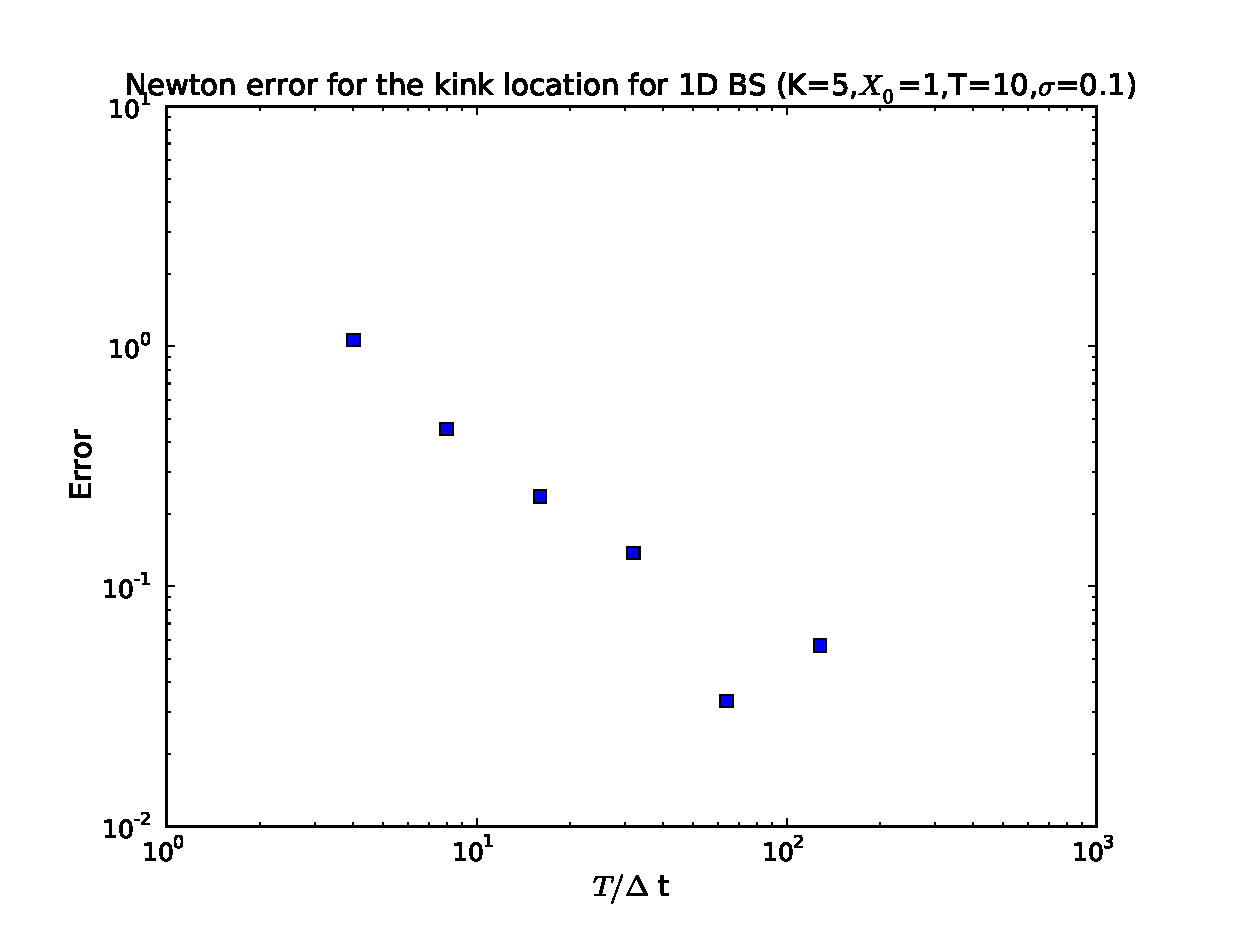
\includegraphics[scale=0.5]{./figures/kink_location_1D_BS_out_the_money.eps}
%\label{fig:1}
%\end{center}
%\end{figure}
%
%\begin{figure}[!h]
%	\begin{center}
%		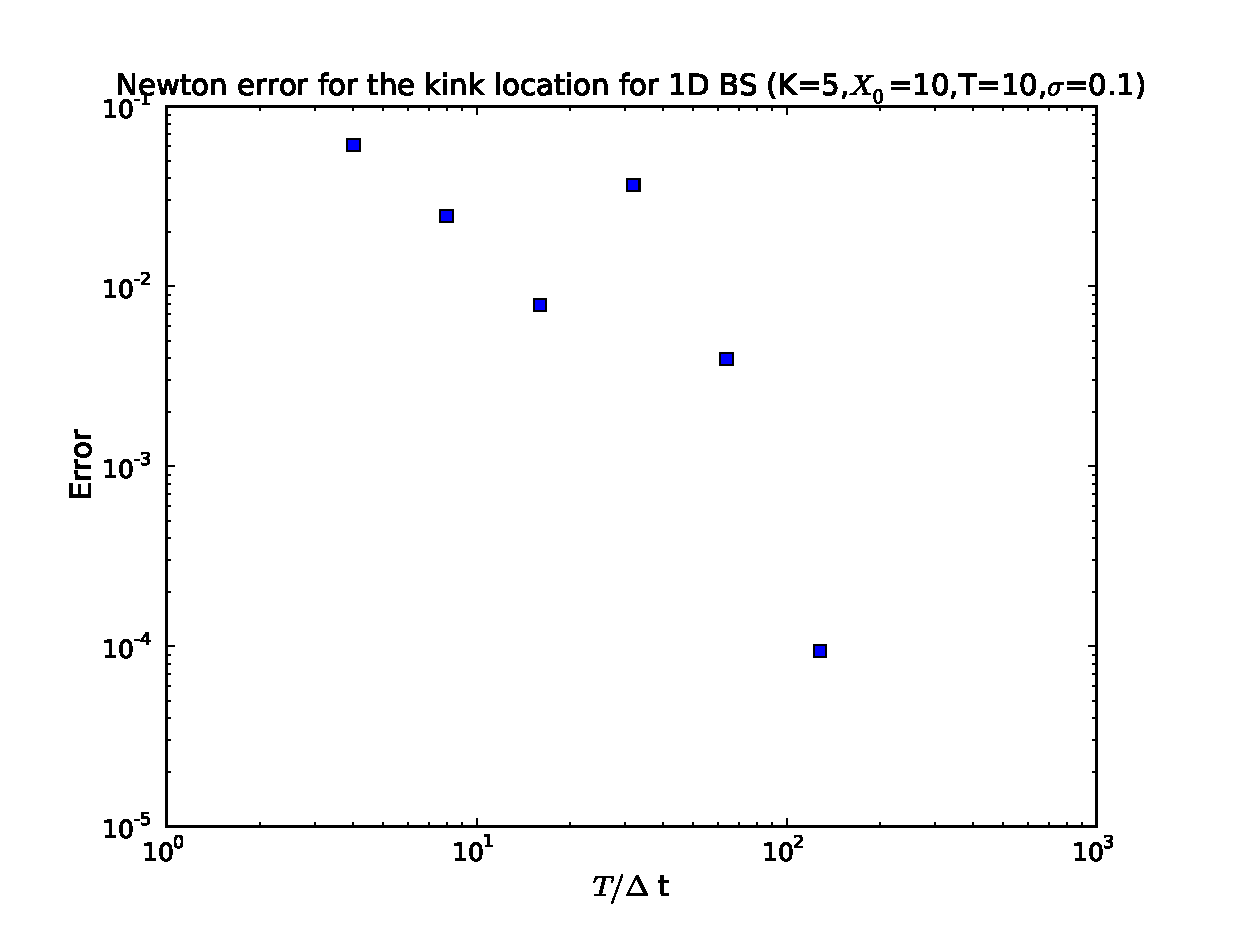
\includegraphics[scale=0.5]{./figures/kink_location_1D_BS_in_the_money.eps}
%		\label{fig:2}
%	\end{center}
%\end{figure}
%
%
%\begin{figure}[!h]
%	\begin{center}
%		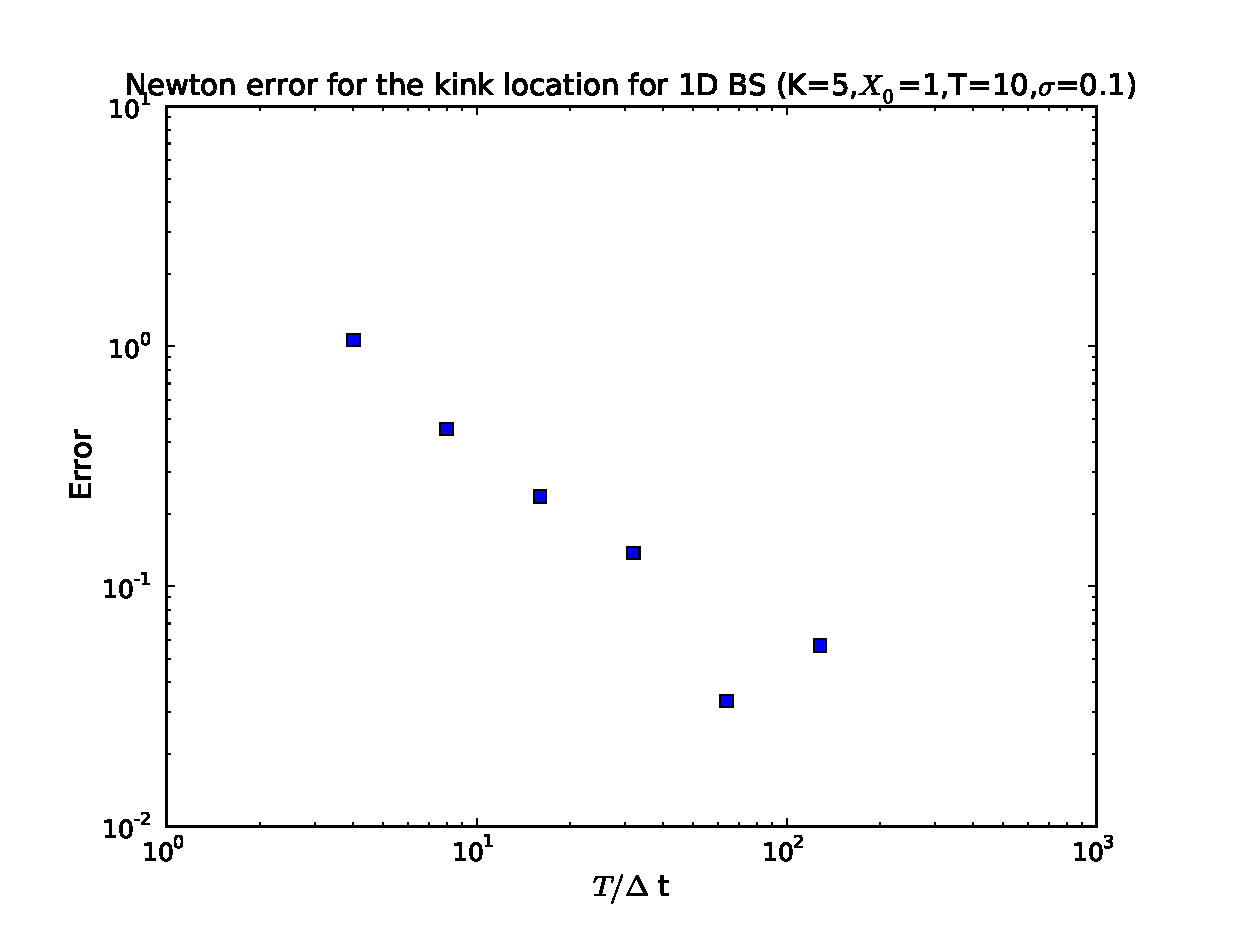
\includegraphics[scale=0.5]{./figures/kink_location_1D_BS_out_the_money.eps}
%		\label{fig:3}
%	\end{center}
%\end{figure}
%
%
%
%
%\newpage
%
%







%\begin{figure}[!h]
%	\centering
%	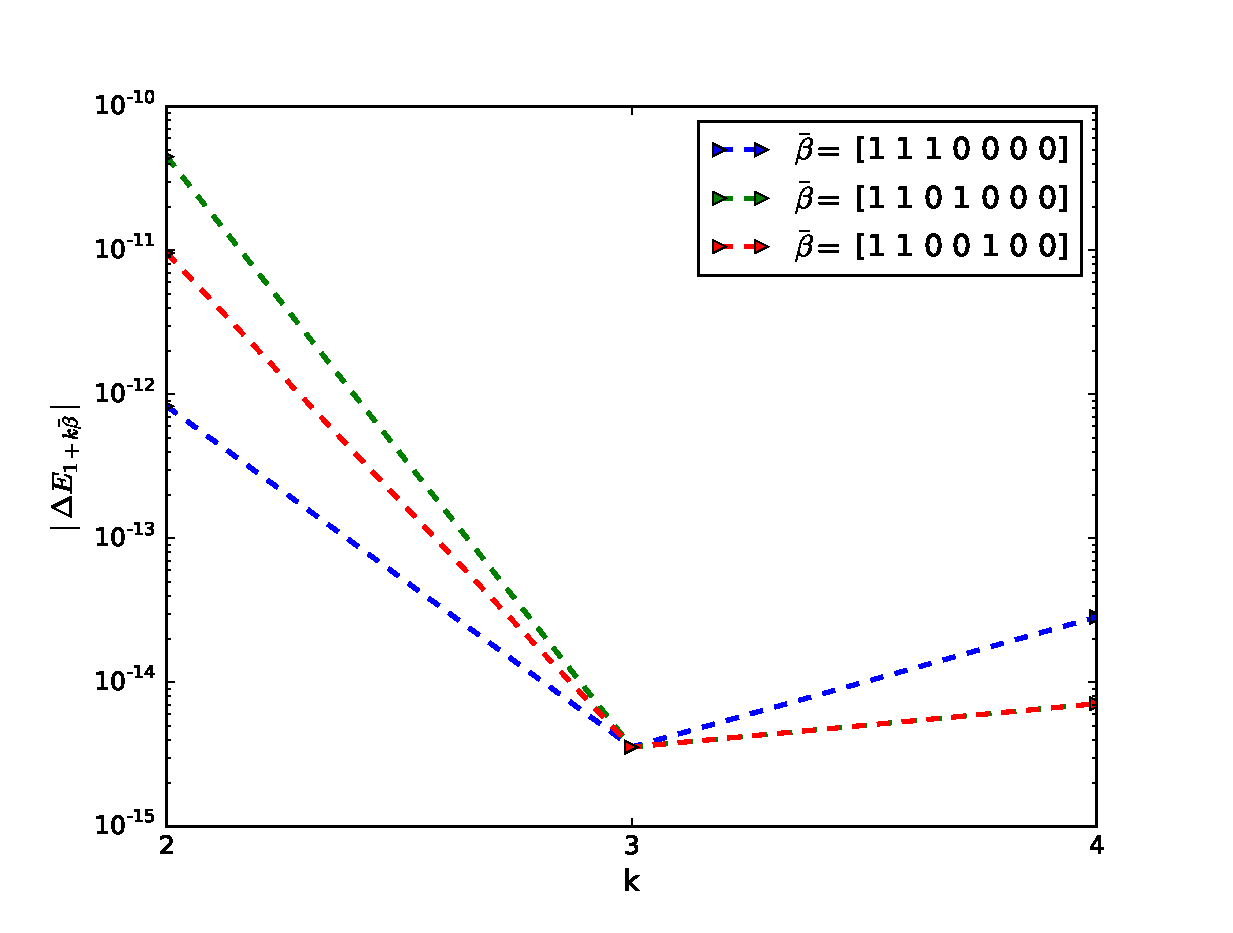
\includegraphics[width=0.6\linewidth]{./figures/mixed_difference_order3_1D_BS_N_8.eps}
%	
%	\caption{The rate of convergence of  third order mixed differences of  $\abs{\Delta E_{\beta}}$ ($\beta=\mathbf{1}+k \bar{\beta}$)): for  $N=8$.}
%	\label{fig:test6}
%\end{figure}





\subsection{Results for the binary option example}\label{sec:Results for the binary option example}

In this case, the integrand $h(\mathbf{z}_{-1})$ is given by

\begin{align}\label{smoothed_integrand_binary_opt_2}
	h(\mathbf{z}_{-1})&= \int \mathbf{1}_{\Phi \circ \Psi(T;z_1,\mathbf{z}_{-1})>K}\frac{1}{\sqrt{2 \pi}} \operatorname{exp} (-z_1^2/2) dy \nonumber\\
	&=  P(Y>y_{\ast}(K)) ,
\end{align}
 
where  $y_{\ast}(x)$, is an invertible function that satisfies 
\begin{align}
	\Phi \circ \Psi (T;y_{\ast}(x),\mathbf{z}_{-1})=x	
\end{align}

We get the kink point by running Newton iteration with a precision of $10^{-10}$.

The paramters that we used in our numerical experiments are: $T=1$, $\sigma=0.4$ and $S_0=K=100$. The exact value of this case is $0.42074029$.

\subsubsection{Weak error plots} \label{sec:Weak error plots_binary}
In this section, we include the results of weak error rates, for the binary option example, for $2$ scenarios, without/with Richardson extrapolation (level $1$). We note that the weak errors plotted here correspond to relative errors.  The upper and lower bounds are $95\%$ confidence interval.

From figure \ref{fig:Weak_rate_binary_without_rich}, we see that we get a weak error of order $\Delta t$. From figure \ref{fig:fig:Weak_rate_binary_with_rich}, we observe an improvement in the rate and the constant when using level $1$ of Richardson extrapolation. The corresponding values of the Bias are reported in tables (\ref{Bias and Statistical errors of MC  for computing Binary option price  for different number of time steps, without Richardson extrapolation. The numbers between parentheses are the corresponding absolute errors.},\ref{Bias and Statistical errors of MC  for computing Binary option price  for different number of time steps, with Richardson extrapolation (level $1$). The numbers between parentheses are the corresponding absolute errors.}).


\begin{figure}[h!]
	\centering
	\begin{subfigure}{.4\textwidth}
		\centering
		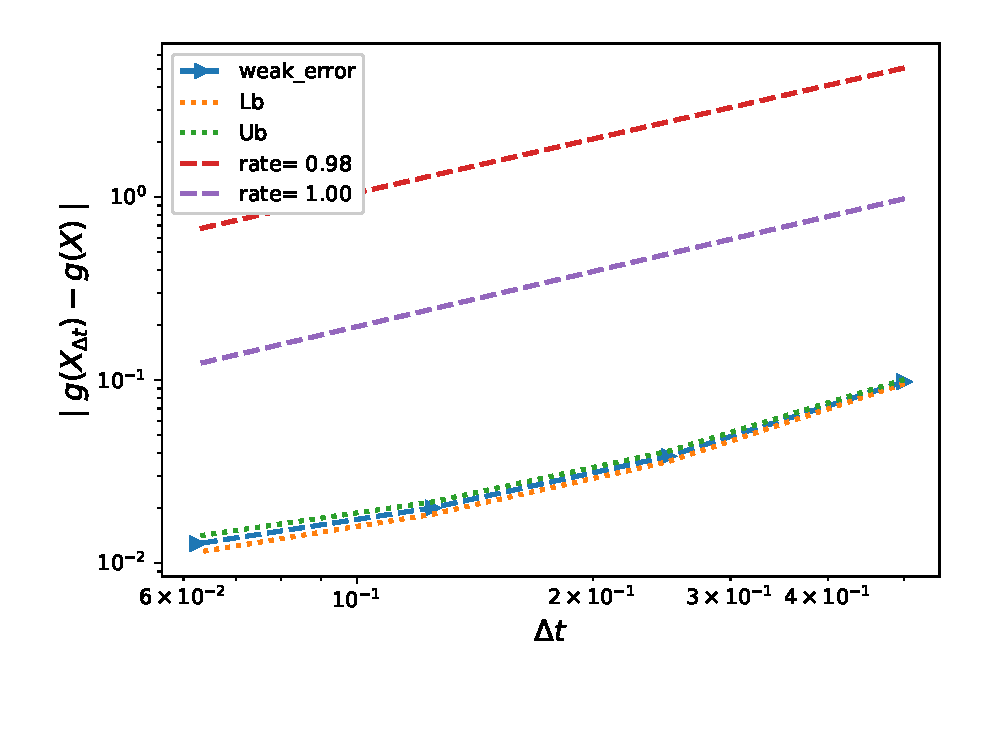
\includegraphics[width=1\linewidth]{./figures/binary_weak_error/without_richardson/weak_convergence_order_binary_option_relative_M_10_4}
		\caption{}
		\label{fig:sub3}
	\end{subfigure}%
	\begin{subfigure}{.4\textwidth}
		\centering
		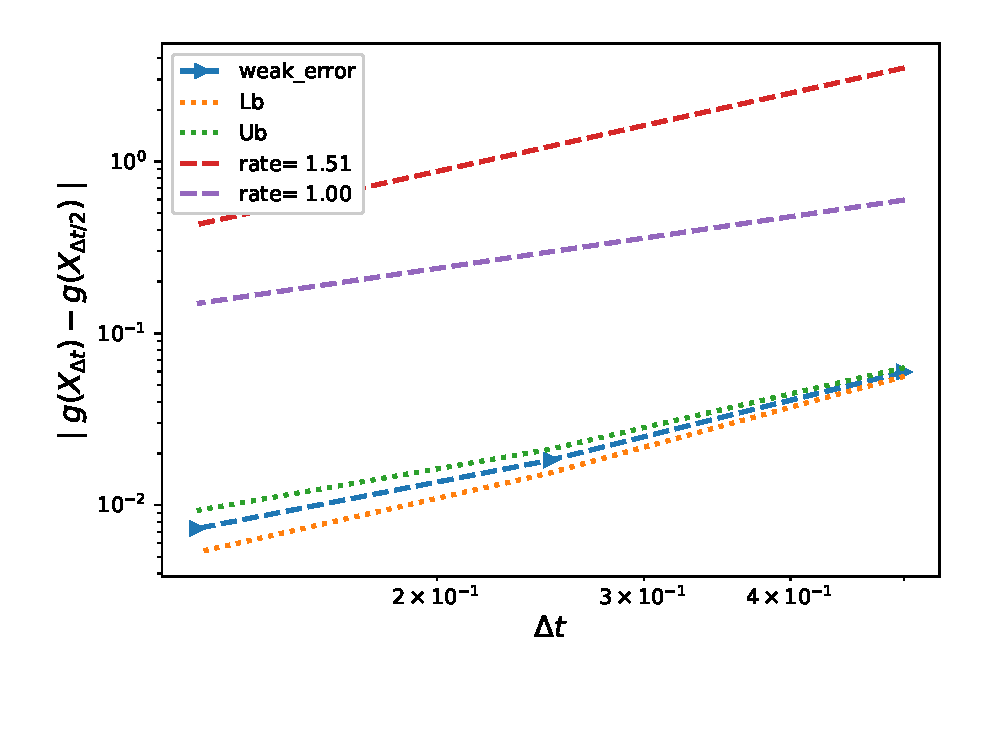
\includegraphics[width=1\linewidth]{./figures/binary_weak_error/without_richardson/weak_convergence_order_differences_binary_option_relative_M_10_4}
		\caption{}
		\label{fig:sub4}
	\end{subfigure}
	
	\caption{The rate of convergence of the weak error for the binary option, without Richardson extraploation, using MC with $M=10^4$: a) $\abs{\expt{g(X_{\Delta t})}-g(X)}$  b) $\abs{\expt{g(X_{\Delta t})-g(X_{\Delta t/2})}}$ }
	\label{fig:Weak_rate_binary_without_rich}
\end{figure}
\begin{figure}[h!]
	\centering
	\begin{subfigure}{.4\textwidth}
		\centering
		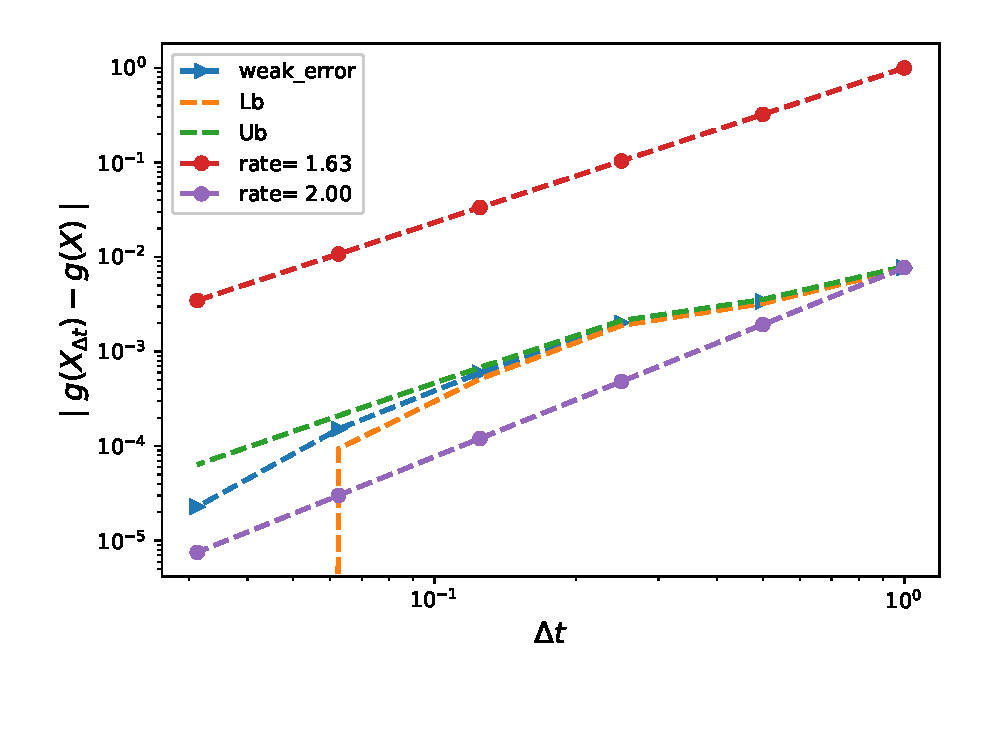
\includegraphics[width=1\linewidth]{./figures/binary_weak_error/with_richardson/weak_convergence_order_binary_richardson_relative_M_5_10_6}
		\caption{}
		\label{fig:sub3}
	\end{subfigure}%
	\begin{subfigure}{.4\textwidth}
		\centering
		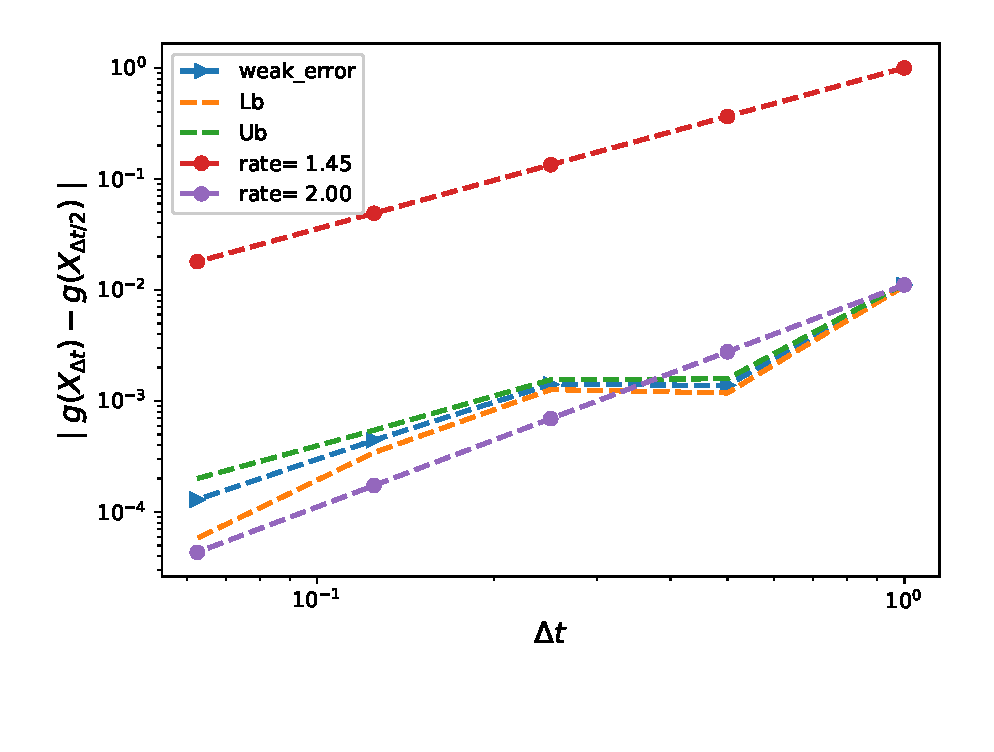
\includegraphics[width=1\linewidth]{./figures/binary_weak_error/with_richardson/weak_convergence_order_differences_binary_richardson_relative_M_5_10_6}
		\caption{}
		\label{fig:sub4}
	\end{subfigure}
	
	\caption{The rate of convergence of the weak error for the binary option, with Richardson extraploation (level 1), using MC with $M=5.10^6$: a) $\abs{\expt{2 g(X_{\Delta t/2}) -g(X_{\Delta t})}-g(X)}$  b) $\abs{\expt{3 g(X_{\Delta t/2})-g(X_{\Delta t})-2 g(X_{\Delta t/4})}}$ }
	\label{fig:fig:Weak_rate_binary_with_rich}
\end{figure}



%\begin{figure}[h!]
%	\centering
%	\begin{subfigure}{.4\textwidth}
%		\centering
%		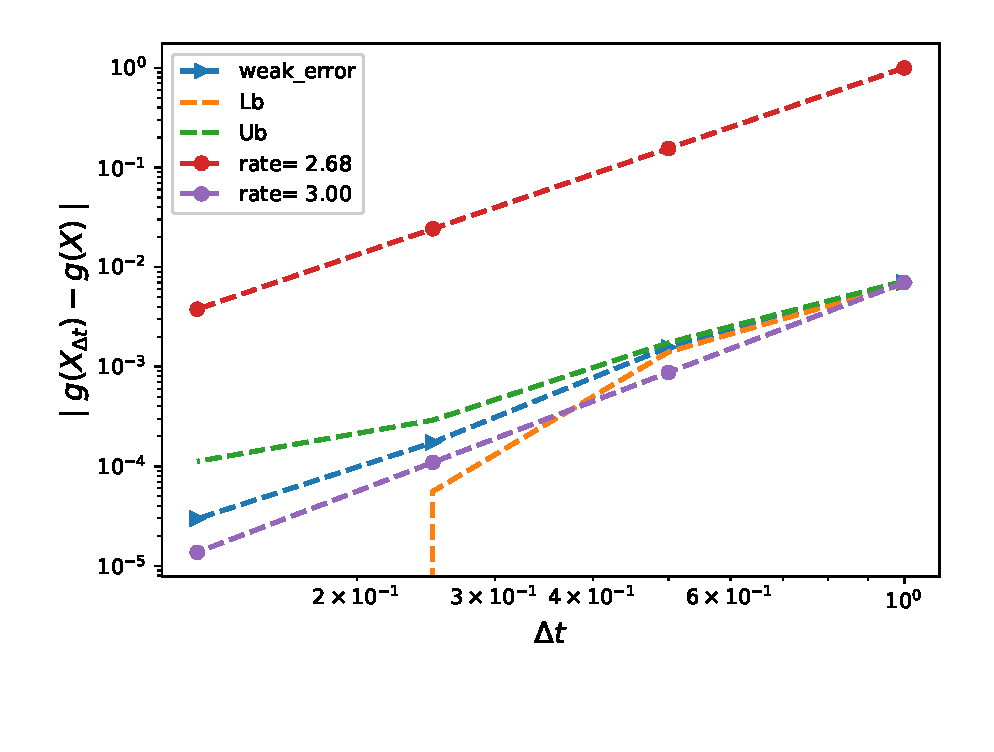
\includegraphics[width=1\linewidth]{./figures/binary_weak_error/with_richardson/weak_convergence_order_binary_richardson_level2_relative_M_5_10_6}
%		\caption{}
%		\label{fig:sub3}
%	\end{subfigure}%
%	\begin{subfigure}{.4\textwidth}
%		\centering
%		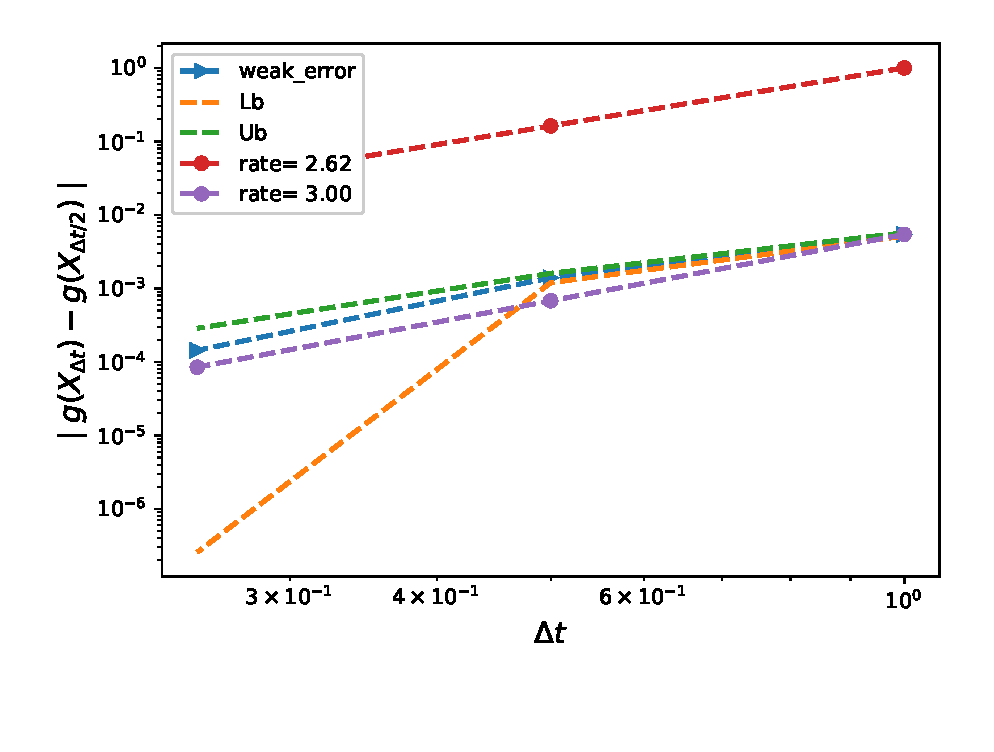
\includegraphics[width=1\linewidth]{./figures/binary_weak_error/with_richardson/weak_convergence_order_differences_binary_richardson_level2_relative_M_5_10_6}
%		\caption{}
%		\label{fig:sub4}
%	\end{subfigure}
%	
%	\caption{The rate of convergence of the weak error for the binary option, with Richardson extraploation (level $2$), using MC with $M=5.10^6$: a) $\abs{\frac{1}{3}\expt{8 g(X_{\Delta t/4}) -6g(X_{\Delta t/2}) +g(X_{\Delta t})}-g(X)}$  b) $\abs{\frac{1}{3}\expt{-8 g(X_{\Delta t/8}) +14g(X_{\Delta t/4})-7 (X_{\Delta t/2}) +g(X_{\Delta t})}}$ }
%	\label{fig:fig:Weak_rate_binary_with_rich_level2}
%\end{figure}
\FloatBarrier
\subsubsection{Comparing relative errors}\label{sec:Comparing relative errors, binary}


\subsubsection*{Without Richardson extrapolation}


In this Section, we report the results for the binary option, using the different Methods: MISC, MC $+$ root finding  and MC, without Richardson extrapolation . We mention that for MISC we used a very small tolerance for the Newton solver, when solving the Kink point problem ($TOL_{\text{Newton}}=10^{-10}$). We start by reporting the observed approximated values using different methods (See table \ref{table: Binary option price of the different methods for different number of time steps, without Richardson extrapolation.}.The biased values for MC method were computed using the values of Bias, reported in table \ref{Bias and Statistical errors of MC  for computing Binary option price  for different number of time steps, without Richardson extrapolation. The numbers between parentheses are the corresponding absolute errors.}. In table \ref{Quadrature error of MISC to compute Binary option price of the different tolerances for different number of time steps, without Richardson extrapolation. The numbers between parentheses are the corresponding absolute errors.}, we report the behavior of quadrature error with respect to MISC tolerance. We precise that the quadrature error is computed by substracting the MISC approximated value from the biased MC value. We report in red the values where MISC becomes stable (see also figure \ref{fig:Quadrature_error_non_rich_binary}). Those values where used to compute the needed number of samples for MC (with and without root finding), to achieve similar magnitude  for statistical error. Later, in table \ref{Total error of MISC and MC to compute Binary option price of the different tolerances for different number of time steps, without Richardson extrapolation. The numbers between parentheses are the corresponding absolute errors.}, we report the total relative error for all methods (Quadrature error + Bias for MISC and Statistical error + Bias for MC). We also report in table \ref{Comparsion of the computational time of  MC and MISC, used to compute Binary option price  for different number of time steps, without Richardson extrapolation}, the computational time needed for all different methods.  We finally provide in figure \ref{fig:Complexity plot for MC and MISC , Binary, Non rich}, the complexity rates for the different involved methods.
\begin{table}[h!]
	\centering
	\begin{tabular}{l*{6}{c}r}
		Method \textbackslash  Steps            & $2$ & $4$ & $8$ & $16$ &   \\
		\hline
		MISC ($TOl=5.10^{-1}$)  & $0.4620$ & $0.4404$ & $0.4299$ & $0.4250$  \\
		MISC ($TOl=10^{-1}$)  & $0.4620$ & $0.4404$ & $0.4301$ & $0.4250$  \\
		MISC ($TOl=5.10^{-2}$)  & $0.4620$ & $0.4403$ & $0.4300$ & $0.4250$  \\
		MISC ($TOl=10^{-2}$)  & $0.4620$ & $0.4406$ &  $0.4300$ & $0.4250$  \\
		MISC ($TOl=10^{-3}$)  & $0.4620$ & $0.4406$ & $0.4301$  & $0.4254$  \\
		MISC ($TOl=10^{-4}$)  & $0.4620$ & $0.4406$ &  $0.4301$ & $-$  \\
		\hline
	%	MC method ($M=10^{5}$)   & $-$ & $-$  & $-$ & $-$ \\		
		MC method ($M=10^{4}$)   & $  0.4620$ & $    0.4369
		$  & $      0.4292$ & $  
		0.4261$ \\	
		\hline
	\end{tabular}
	\caption{Binary option price of the different methods for different number of time steps, without Richardson extrapolation.}
	\label{table: Binary option price of the different methods for different number of time steps, without Richardson extrapolation.}
\end{table}

\begin{table}[h!]
	\centering
	\begin{tabular}{l*{6}{c}r}
		Method \textbackslash  Steps            & $2$ & $4$ & $8$ & $16$  \\
		\hline
		MC Bias $(M=10^{4})$  & 	$ \underset{(    
			0.0412)}{\mathbf{0.0980}}$  & $\underset{( 0.0162)}{\mathbf{ 0.0384
		}}$  & $\underset{(    0.0085
	)}{\mathbf{0.0201}}$ & $\underset{(   0.0053)}{\mathbf{   0.0127}}$\\ 
		
		MC Statistical error $(M=10^{4})$  &  $\underset{( 5.0e-04)} {\mathbf{1.2e-03}}$  & $\underset{( 5.0e-04)} {\mathbf{1.2e-03}}$ & $\underset{(3.4e-04)} {\mathbf{8.0e-04}}$ & $\underset{( 2.7e-04)} {\mathbf{6.5e-04}}$	\\
%			MC: Statistical error ($M=10^6$)  &  $\underset{( 5.0e-04)} {\mathbf{1.2e-03}}$  & $\underset{( 5.0e-04)} {\mathbf{1.2e-03}}$ & $\underset{( 5.0e-04)} {\mathbf{1.2e-03}}$ & $\underset{( 5.0e-04)} {\mathbf{1.2e-03}}$	\\
		\hline
	\end{tabular}
	\caption{Bias and Statistical errors of MC  for computing Binary option price  for different number of time steps, without Richardson extrapolation. The numbers between parentheses are the corresponding absolute errors.}
	\label{Bias and Statistical errors of MC  for computing Binary option price  for different number of time steps, without Richardson extrapolation. The numbers between parentheses are the corresponding absolute errors.}
\end{table}





\begin{table}[h!]
	\centering
	\begin{tabular}{l*{6}{c}r}
		Method \textbackslash  Steps            & $2$ & $4$ & $8$ & $16$  \\
		\hline
		MISC ($TOl=5.10^{-1}$)  & $\underset{(2.4e-05)}{\mathbf{\red{1.0e-05}}}$ & $\underset{(0.0035)}{\mathbf{0.0083}}$  & $\underset{(0.0007)}{\mathbf{ 0.0017}}$ &$\underset{(0.0011)}{\mathbf{0.0026}}$ \\
		MISC ($TOl=10^{-1}$)   & $\underset{(2.4e-05)}{\mathbf{1.0e-05}}$ & $\underset{(0.0035)}{\mathbf{0.0083}}$ & $\underset{(0.0009)}{\mathbf{\red{0.0021}}}$ & $\underset{(0.0011)}{\mathbf{
				0.0026}}$ \\
		MISC ($TOl=5.10^{-2}$)  & $\underset{(2.4e-05)}{\mathbf{1.0e-05}}$& $\underset{(0.0034)}{\mathbf{0.0081}}$ & $\underset{(0.0008)}{\mathbf{ 0.0019}}$& $\underset{(0.0011)}{\mathbf{
				0.0026}}$ \\
		MISC ($TOl=10^{-2}$)  & $\underset{(2.4e-05)}{\mathbf{1.0e-05}}$ & $\underset{(0.0037)}{\mathbf{\red{0.0088}}}$ & $\underset{(0.0008)}{\mathbf{ 0.0019}}$ & $\underset{(0.0011)}{\mathbf{
				0.0026}}$ \\
		MISC ($TOl=10^{-3}$)  & $\underset{(2.4e-05)}{\mathbf{1.0e-05}}$ & $\underset{(0.0037)}{\mathbf{0.0088}}$& $\underset{(0.0009)}{\mathbf{0.0021}}$& $\underset{(0.0007)}{\mathbf{\red{ 0.0017}}}$ \\
			MISC ($TOl=10^{-4}$)  & $\underset{(2.4e-05)}{\mathbf{1.0e-05}}$ & $\underset{(0.0037)}{\mathbf{0.0088}}$& $\underset{(0.0009)}{\mathbf{0.0021}}$& $\underset{(-)}{\mathbf{ -}}$ \\
		\hline
	\end{tabular}
	\caption{Quadrature error of MISC to compute Binary option price of the different tolerances for different number of time steps, without Richardson extrapolation. The numbers between parentheses are the corresponding absolute errors.}
	\label{Quadrature error of MISC to compute Binary option price of the different tolerances for different number of time steps, without Richardson extrapolation. The numbers between parentheses are the corresponding absolute errors.}
\end{table}


	\begin{figure}[h!]
	\centering
	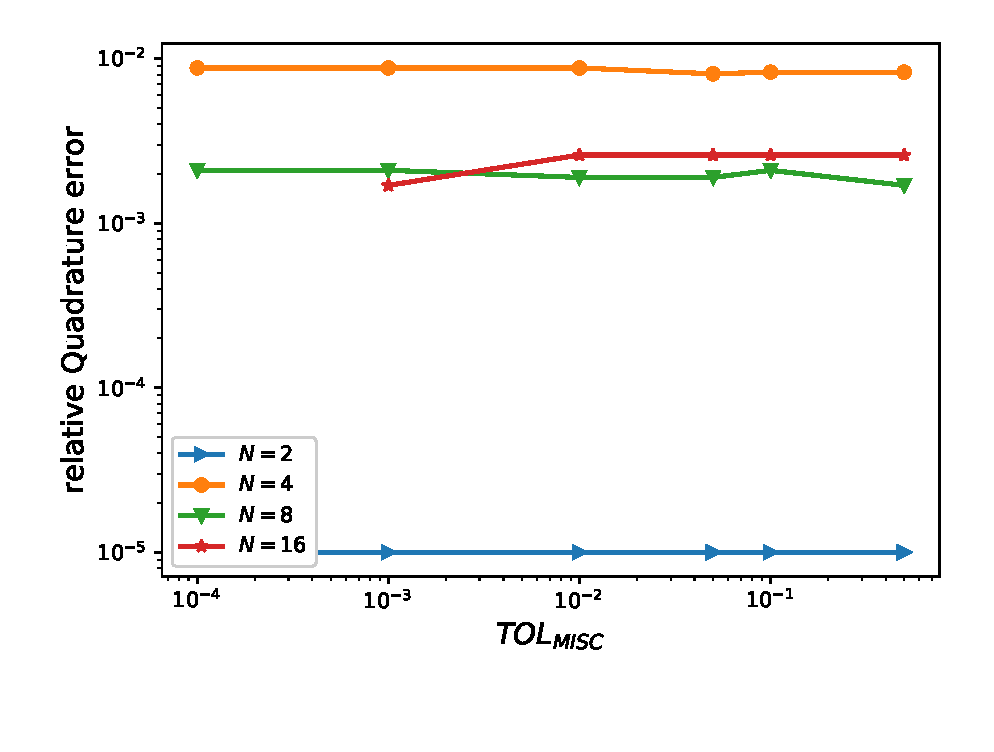
\includegraphics[width=0.7\linewidth]{./figures/Binary_MISC_quadrature_error/relative_quad_error_wrt_MISC_TOL_non_rich}
	
	
	\caption{Relative quadrature error of MISC to compute Binary option price of the different tolerances for different number of time steps, without Richardson extrapolation.}
	\label{fig:Quadrature_error_non_rich_binary}
\end{figure}





\begin{table}[h!]
	\centering
	\begin{tabular}{l*{6}{c}r}
		Method \textbackslash  Steps            & $2$ & $4$ & $8$ & $16$  \\
		\hline
		MISC ($TOl=5.10^{-1}$)  & $\mathbf{\red{0.0980}}$ & $\mathbf{0.0467}$ & $\mathbf{ 0.0218}$ & $\mathbf{0.0153}$  \\
		MISC ($TOl=10^{-1}$)  &$\mathbf{0.0980}$& $\mathbf{0.0467}$ & $\mathbf{\red{0.0222}}$ & $\mathbf{0.0153}$   \\
		MISC ($TOl=5.10^{-2}$) & $\mathbf{0.0980}$ & $\mathbf{0.0465}$ & $\mathbf{0.0220}$ & $\mathbf{0.0153}$  \\
		MISC ($TOl=10^{-2}$)  & $\mathbf{0.0980}$ & $\mathbf{\red{ 0.0472}}$ & $\mathbf{ 0.0220}$ & $\mathbf{0.0153}$    \\
		MISC ($TOl=10^{-3}$)  & $\mathbf{0.0980}$  & $\mathbf{ 0.0472}$  & $\mathbf{ 0.0222}$  & $\mathbf{\red{0.0144}}$\\
	MISC ($TOl=10^{-4}$)  & $\mathbf{0.0980}$ & $\mathbf{0.0472}$ & $\mathbf{ 0.0222}$ & $\mathbf{-}$  \\
		\hline
		MC+root finding   &  $\mathbf{\red{-}}$ & $\mathbf{\red{0.0471 }}$ & $\mathbf{\red{0.0221}}$ & $\mathbf{\red{0.0141}}$  \\	
			MC     &  $\mathbf{\red{-}}$ & $\mathbf{\red{0.0467}}$ & $\mathbf{\red{0.0222}}$ & $\mathbf{\red{0.0146}}$  \\	
		\hline
	
	\end{tabular}
	\caption{Total error of MISC and MC to compute Binary option price of the different tolerances for different number of time steps, without Richardson extrapolation. The numbers between parentheses are the corresponding absolute errors. We will not include later the first point, corresponding to number of time steps $N=2$, since as from table \ref{Quadrature error of MISC to compute Binary option price of the different tolerances for different number of time steps, without Richardson extrapolation. The numbers between parentheses are the corresponding absolute errors.}, MISC is killing the quadrature error for that case.}
	\label{Total error of MISC and MC to compute Binary option price of the different tolerances for different number of time steps, without Richardson extrapolation. The numbers between parentheses are the corresponding absolute errors.}
\end{table}




\begin{table}[h!]
	\centering
	\begin{tabular}{l*{6}{c}r}
		Method \textbackslash  Steps            & $2$ & $4$ & $8$ & $16$ &   \\
		\hline
		MISC ($TOl=5.10^{-1}$)  & $\red{0.3}$ & $0.8$ & $2$ & $9$  \\
		MISC ($TOl=10^{-1}$)   & $0.3$ & $0.8$ & $\red{9}$ & $49$  \\
		MISC ($TOl=5.10^{-2}$)   & $0.3$ & $1.3$ & $12$ & $59$  \\
		MISC ($TOl=10^{-2}$)   & $0.3$ & $\red{2}$ & $14$ & $63$  \\
		MISC ($TOl=10^{-3}$)   & $0.3$ & $2$ & $34$ & $\red{1090}$  \\
    	MISC ($TOl=10^{-4}$)   & $0.3$ & $16$ & $193$ & $-$  \\
		\hline
		MC+root finding method    & $\red{-}$ & $\red{9}$ & $\red{96}$ & $\red{141}$  \\
		MC method    & $\red{-}$ & $\red{7}$ & $\red{95}$ & $\red{152}$  \\
		\hline
		Ratio of	$\text{(MC+root finding)}/\text{(MISC)}$ & $\red{-}$ & $\red{4.5}$ & $\red{11}$ & $\red{0.13}$  \\
			Ratio of	$(\text{MC})/(\text{MISC})$ & $\red{-}$ & $\red{3.5}$ & $\red{11}$ & $\red{0.14}$  \\
			\hline
	\end{tabular}
	\caption{Comparsion of the computational time of  MC and MISC, used to compute Binary option price  for different number of time steps, without Richardson extrapolation. The average computational time of MC is computed over $10$ runs.}
	\label{Comparsion of the computational time of  MC and MISC, used to compute Binary option price  for different number of time steps, without Richardson extrapolation}
\end{table}





	\begin{figure}[h!]
	\centering
	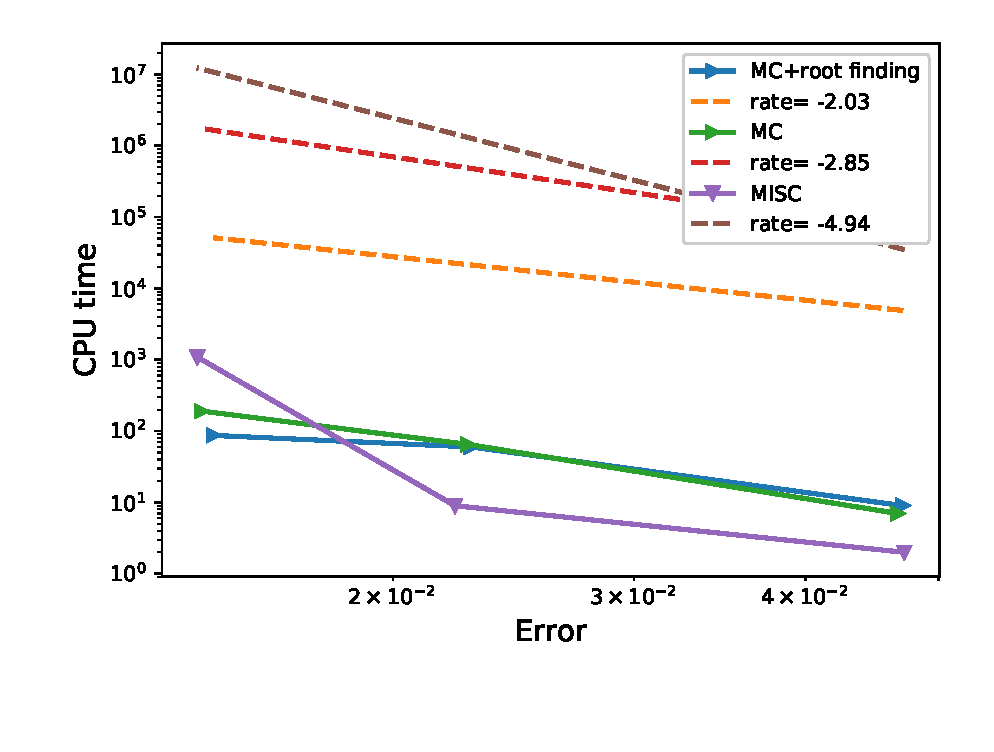
\includegraphics[width=0.7\linewidth]{./figures/Binary_Complexity_rates/error_vs_time}
	
	\caption{Complexity plot for MC and MISC for the case without Richardson extrapolation.}
	\label{fig:Complexity plot for MC and MISC , Binary, Non rich}
\end{figure}

\FloatBarrier

\subsubsection*{With Richardson extrapolation (level $1$)}
In this Section, we report the results for the binary option, using the different Methods: MISC, MC $+$ root finding  and MC, with Richardson extrapolation . We mention that for MISC we used a very small tolerance for the Newton solver, when solving the Kink point problem ($TOL_{\text{Newton}}=10^{-10}$). We start by reporting the observed approximated values using different methods (See table \ref{table: Binary option price of the different methods for different number of time steps, with Richardson extrapolation (level1).}. The biased values for MC method were computed using the values of Bias, reported in table \ref{Bias and Statistical errors of MC  for computing Binary option price  for different number of time steps, with Richardson extrapolation (level $1$). The numbers between parentheses are the corresponding absolute errors.}. In table \ref{Quadrature error of MISC to compute Binary option price of the different tolerances for different number of time steps, with Richardson extrapolation (level $1$). The numbers between parentheses are the corresponding absolute errors.}, we report the behavior of quadrature error with respect to MISC tolerance. We precise that the quadrature error is computed by substracting the MISC approximated value from the biased MC value. We report in red the values where MISC becomes stable (see also figure \ref{fig:Quadrature_error_with_rich_binary}). Those values where used to compute the needed number of samples for MC (with and without root finding), to achieve similar magnitude  for statistical error. Later, in table \ref{Total error of MISC and MC to compute Binary option price of the different tolerances for different number of time steps, with Richardson extrapolation (level $1$). The numbers between parentheses are the corresponding absolute errors.}, we report the total relative error for all methods (Quadrature error + Bias for MISC and Statistical error + Bias for MC). We also report in table\ref{Comparsion of the computational time of  MC and MISC, used to compute Binary option price  for different number of time steps, with Richardson extrapolation (level $1$)}, the computational time needed for all different methods.  We finally provide in figure \ref{fig:Complexity plot for MC and MISC , Binary, with rich}, the complexity rates for the different involved methods, as well a comparison between the two versions of MISC (without/with Richardson extrapolation) in figure \ref{fig:Complexity plot for MC and MISC , Binary, comparison}.
\begin{table}[h!]
	\centering
	\begin{tabular}{l*{6}{c}r}
		Method \textbackslash  Steps            & $1-2$ & $2-4$ & $4-8$ & $8-16$ &   \\
		\hline
		MISC ($TOl=5.10^{-1}$)  & $0.4239$ & $0.4188$ & $0.4191$ & $0.4200$  \\
		MISC ($TOl=10^{-1}$)  &$0.4239$ & $0.4188$ &$0.4191$ & $0.4199$  \\
		MISC ($TOl=5.10^{-2}$) & $0.4239$ & $0.4188$ & $0.4190$ & $0.4199$  \\
		MISC ($TOl=10^{-2}$) &$0.4239$ & $0.4192$ & $0.4194$ & $0.4199$  \\
		MISC ($TOl=10^{-3}$) & $0.4239$ & $0.4192$ & $0.4199$ & $0.4205$  \\
			MISC ($TOl=10^{-4}$) & $0.4239$ & $0.4193$ & $0.4199$ & $-$  \\
		\hline
		MC method ($M=5.10^{6}$)   & $ 0.4240$ & $
		0.4224$ & $    0.4216$ & $  0.4210$  \\
		\hline
	\end{tabular}
	\caption{Binary option price of the different methods for different number of time steps, with Richardson extrapolation (level $1$).}
	\label{table: Binary option price of the different methods for different number of time steps, with Richardson extrapolation (level1).}
\end{table}


\begin{table}[h!]
	\centering
	\begin{tabular}{l*{6}{c}r}
		Method \textbackslash  Steps            & $1-2$ & $2-4$ & $4-8$ & $8-16$  \\
		\hline
	MC Bias  ($M=5.10^{6}$)&$ \underset{(0.0032)}{\mathbf{0.0077}}$    & $\underset{(    0.0016
		)}{\mathbf{0.0039}}$  & $\underset{(0.0008)}{\mathbf{0.0020}}$  & $\underset{(0.0003)}{\mathbf{0.0006}}$\\
		MC Statistical error   ($M=5.10^{6}$)   & 	$ \underset{( 4.6e-05  )}{\mathbf{1.1e-04}}$  & $\underset{(3.5e-05)}{\mathbf{ 8.4e-05
	}}$  & $\underset{(2.5e-05)}{\mathbf{6.0e-05}}$ & $\underset{(   1.8e-05 )}{\mathbf{  4.2e-05 }}$\\ 
		
%		MC+root finding: Statistical error ($M=10^3$)     & 	$ \underset{( 3.5e-03  )}{\mathbf{8.3e-03}}$  & $\underset{(2.8e-03)}{\mathbf{ 6.6e-03
%		}}$  & $\underset{(1.8e-03)}{\mathbf{4.3e-03}}$ & $\underset{(  1.2e-03 )}{\mathbf{  2.9e-03 }}$\\ 
%		
		\hline
	\end{tabular}
	\caption{Bias and Statistical errors of MC  for computing Binary option price  for different number of time steps, with Richardson extrapolation (level $1$). The numbers between parentheses are the corresponding absolute errors.}
	\label{Bias and Statistical errors of MC  for computing Binary option price  for different number of time steps, with Richardson extrapolation (level $1$). The numbers between parentheses are the corresponding absolute errors.}
\end{table}




\begin{table}[h!]
	\centering
	\begin{tabular}{l*{6}{c}r}
		Method \textbackslash  Steps            & $1-2$ & $2-4$ & $4-8$ & $8-16$  \\
		\hline
		MISC ($TOl=5.10^{-1}$)  & $\underset{(   1.0e-04)}{\mathbf{ \red{2.4e-04}}}$ & $\underset{(3.6e-03)}{\mathbf{8.6e-03}}$  & $\underset{(2.5e-03)}{\mathbf{5.9e-03}}$ &$\underset{(1.0e-03)}{\mathbf{2.4e-03}}$ \\
		MISC ($TOl=10^{-1}$)   & $\underset{(   1.0e-04)}{\mathbf{ 2.4e-04}}$ & $\underset{(3.6e-03)}{\mathbf{8.6e-03}}$  & $\underset{(2.5e-03)}{\mathbf{5.9e-03}}$ &$\underset{(   1.1e-04)}{\mathbf{ \red{2.6e-03}}}$ \\
		MISC ($TOl=5.10^{-2}$)  & $\underset{(   1.0e-04)}{\mathbf{ 2.4e-04}}$ & $\underset{(3.6e-03)}{\mathbf{8.6e-03}}$ & $\underset{(2.6e-03)}{\mathbf{6.2e-03}}$ &$\underset{(   1.1e-04)}{\mathbf{ 2.6e-03}}$ \\
		MISC ($TOl=10^{-2}$)  & $\underset{(   1.0e-04)}{\mathbf{ 2.4e-04}}$ & $\underset{(3.2e-03)}{\mathbf{\red{7.6e-03}}}$  & $\underset{(2.2e-03)}{\mathbf{\red{5.2e-03}}}$ &$\underset{(   1.1e-04)}{\mathbf{ 2.6e-03}}$\\
		MISC ($TOl=10^{-3}$)  & $\underset{(   1.0e-04)}{\mathbf{ 2.4e-04}}$ & $\underset{(3.2e-03)}{\mathbf{7.6e-03}}$  & $\underset{(1.7e-03)}{\mathbf{4.0e-03}}$ &$\underset{(   5.e-04)}{\mathbf{1.2e-03}}$ \\
	MISC ($TOl=10^{-4}$)  & $\underset{(   1.0e-04)}{\mathbf{ 2.4e-04}}$ & $\underset{(3.1e-03)}{\mathbf{7.4e-03}}$  & $\underset{(1.7e-03)}{\mathbf{4.0e-03}}$ &$\underset{()}{\mathbf{}}$ \\
		\hline
	\end{tabular}
	\caption{Quadrature error of MISC to compute Binary option price of the different tolerances for different number of time steps, with Richardson extrapolation (level $1$). The numbers between parentheses are the corresponding absolute errors.}
	\label{Quadrature error of MISC to compute Binary option price of the different tolerances for different number of time steps, with Richardson extrapolation (level $1$). The numbers between parentheses are the corresponding absolute errors.}
\end{table}



	\begin{figure}[h!]
	\centering
	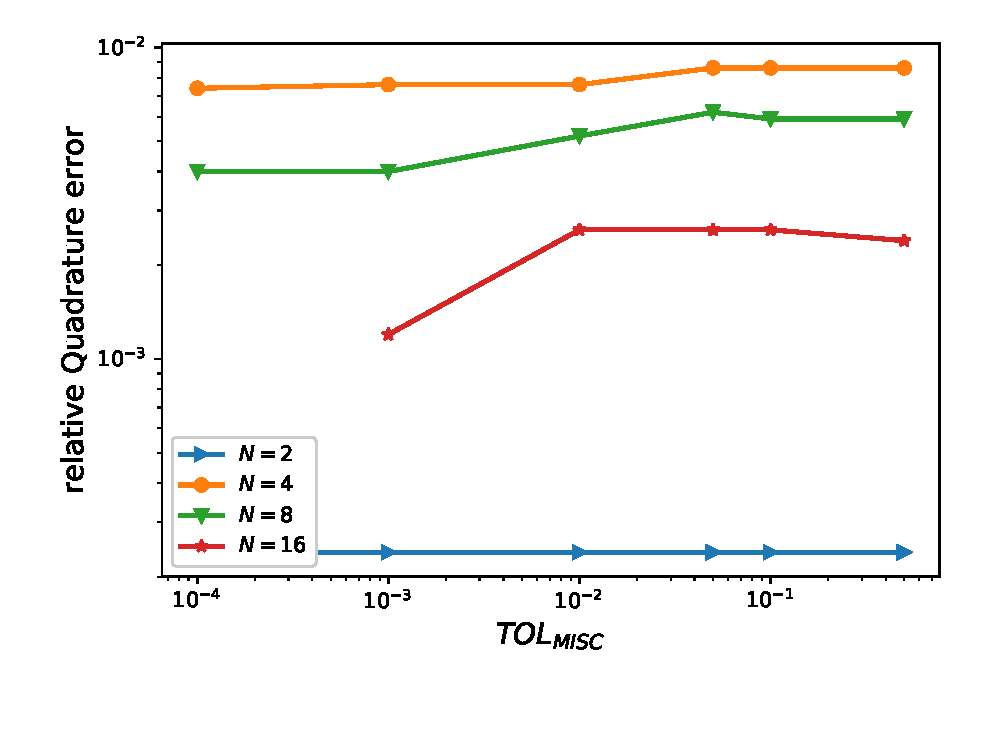
\includegraphics[width=0.7\linewidth]{./figures/Binary_MISC_quadrature_error/relative_quad_error_wrt_MISC_TOL_with_rich}
	
	
	\caption{Relative quadrature error of MISC to compute Binary option price of the different tolerances for different number of time steps, with Richardson extrapolation.}
	\label{fig:Quadrature_error_with_rich_binary}
\end{figure}



\begin{table}[h!]
	\centering
	\begin{tabular}{l*{6}{c}r}
		Method \textbackslash  Steps            & $1-2$ & $2-4$ & $4-8$ & $8-16$  \\
		\hline
		MISC ($TOl=5.10^{-1}$)  &  $\mathbf{\red{0.0079}}$ & $\mathbf{0.0125}$ & $\mathbf{0.0079}$ & $\mathbf{0.0030}$  \\
		MISC ($TOl=10^{-1}$)  &   $\mathbf{0.0079}$& $\mathbf{0.0125}$ & $\mathbf{0.0079}$ & $\mathbf{\red{0.0032}}$  \\
		MISC ($TOl=5.10^{-2}$) &   $\mathbf{0.0079}$ & $\mathbf{0.0125}$ & $\mathbf{0.0082}$ & $\mathbf{0.0032}$  \\
		MISC ($TOl=10^{-2}$)  &   $\mathbf{0.0079}$ & $\mathbf{\red{0.0115}}$ & $\mathbf{\red{0.0072}}$ & $\mathbf{0.0032}$  \\
		MISC ($TOl=10^{-3}$) &   $\mathbf{0.0079}$ & $\mathbf{0.0115}$ & $\mathbf{0.0060}$ & $\mathbf{0.0018}$  \\

	MISC ($TOl=10^{-4}$) &   $\mathbf{0.0079}$ & $\mathbf{0.0113}$ & $\mathbf{0.0060}$ & $\mathbf{-}$  \\
		\hline
		MC+root finding   &  $\mathbf{\red{-}}$ & $\mathbf{\red{0.0111}}$ & $\mathbf{\red{0.0070}}$ & $\mathbf{\red{0.0035}}$  \\	
			MC    &  $\mathbf{\red{-}}$ & $\mathbf{\red{0.0116}}$ & $\mathbf{\red{0.0073}}$ & $\mathbf{\red{0.0029}}$  \\	
		\hline
		
	\end{tabular}
	\caption{Total error of MISC and MC to compute Binary option price of the different tolerances for different number of time steps, with Richardson extrapolation (level $1$). The numbers between parentheses are the corresponding absolute errors.  We will not include later the first point, corresponding to number of time steps $N=2$, since as from table \ref{Quadrature error of MISC to compute Binary option price of the different tolerances for different number of time steps, with Richardson extrapolation (level $1$). The numbers between parentheses are the corresponding absolute errors.}, MISC is killing the quadrature error for that case.}
	\label{Total error of MISC and MC to compute Binary option price of the different tolerances for different number of time steps, with Richardson extrapolation (level $1$). The numbers between parentheses are the corresponding absolute errors.}
\end{table}






\begin{table}[h!]
	\centering
	\begin{tabular}{l*{6}{c}r}
		Method \textbackslash  Steps            & $1-2$ & $2-4$ & $4-8$ & $8-16$ &   \\
		\hline
		MISC ($TOl=5.10^{-1}$) & $\red{0.3}$ & $1$ & $4$ & $9$  \\
		MISC ($TOl=10^{-1}$)  & $0.3$& $1$ & $8$ & $\red{42}$  \\
		MISC ($TOl=5.10^{-2}$)   & $0.3$ & $1$ & $10$ & $72$  \\
		MISC ($TOl=10^{-2}$)  & $0.3$ & $\red{4}$ & $\red{15}$ & $78$  \\
		MISC ($TOl=10^{-3}$)   &$0.3$ & $4$ & $100$ & $2253$  \\
			MISC ($TOl=10^{-4}$)   &$0.3$ & $68$ & $392$ & $$  \\
		\hline
		MC+root finding method     & $\red{-}$ & $\red{48}$ & $\red{62}$ & $\red{122 }$  \\
			MC   & $\red{-}$ & $\red{12}$ & $\red{23}$ & $\red{147}$  \\
		\hline
			Ratio of	$\text{(MC+root finding)}/\text{(MISC)}$ & $\red{-}$ & $\red{12}$ & $\red{4.1}$ & $\red{2.9}$  \\
		Ratio of	$(\text{MC})/(\text{MISC})$ & $\red{-}$ & $\red{3}$ & $\red{1.5}$ & $\red{3.5}$  \\
		\hline
	\end{tabular}
	\caption{Comparsion of the computational time of  MC and MISC, used to compute Binary option price  for different number of time steps, with Richardson extrapolation (level $1$). The average computational time of MC is computed over $10$ runs.}
	\label{Comparsion of the computational time of  MC and MISC, used to compute Binary option price  for different number of time steps, with Richardson extrapolation (level $1$)}
\end{table}


	\begin{figure}[h!]
\centering
\includegraphics[width=0.7\linewidth]{./figures/Binary_Complexity_rates/error_vs_time_rich}

\caption{Complexity plot for MC and MISC for the case with Richardson extrapolation.}
\label{fig:Complexity plot for MC and MISC , Binary, with rich}
\end{figure}







\begin{figure}[h!]
\centering
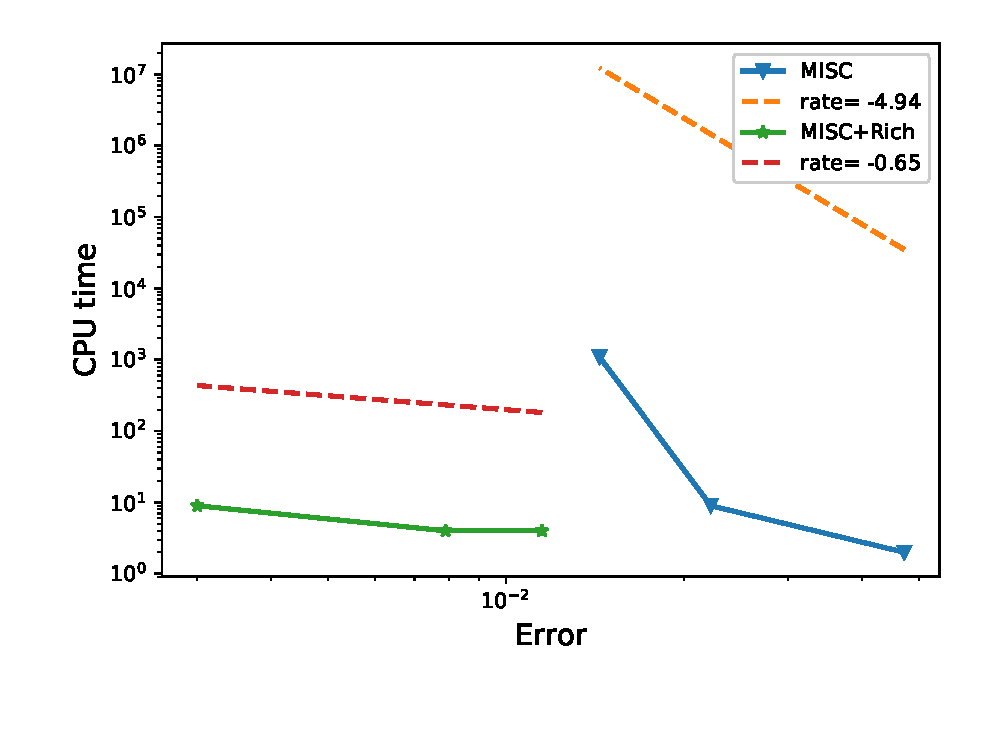
\includegraphics[width=0.7\linewidth]{./figures/Binary_Complexity_rates/error_vs_time_comparison}

\caption{Complexity plot for MISC without and with Richardson extrapolation, for the Binary option.}
\label{fig:Complexity plot for MC and MISC , Binary, comparison}
\end{figure}

\FloatBarrier



%In the following, we compare the  relative errors for the binary option example under Black-Scholes model (see Tables (\ref{Relative error of the binary option price of the different tolerances for different number of time steps.}, \ref{Relative error of Call option price of the different tolerances for different number of time steps, using Richardson extrapolation (level $1$)})). We report the results for $2$ scenarios: i) Without using Richardson extrapolation, ii) Using level $1$ Richardson extrapoaltion.  You may see appendix \ref{appendix:Call prices for different methods_binary} for the values of binary option prices.
%
%Given the normalized bias computed by MC method (See Section \ref{sec:Weak error plots_binary}) (reported as bold values in the tables), we report in red in each table the smallest tolerance that MISC required to get below that relative bias (I do not put values for smaller tolerances, once the required bias is reached).
%
%From the tables (\ref{Relative error of the binary option price of the different tolerances for different number of time steps.}, \ref{Relative error of Call option price of the different tolerances for different number of time steps, using Richardson extrapolation (level $1$)})), we may observe that to get a relative error below $1\%$, we need around $16$ time steps for the case without Richardson extrapolation compared to only using $1$ time step in the coarse level for the case of level $1$ Richardson extraplation. 



%\begin{table}[h!]
%	\centering
%	\begin{tabular}{l*{5}{c}r}
%		Method \textbackslash  Steps    &$1-2$        & $2-4$ & $4-8$ & $8-16$  \\
%		\hline
%		MISC ($TOl=5.10^{-1}$)  &$\red{0.0076}$ & $0.0045$ & $0.0031$ & $0.0017$  \\
%		MISC ($TOl=10^{-2}$)  &$-$ & $\red{0.0036}$ & $0.0031$ & $0.0014$  \\
%		MISC ($TOl=10^{-3}$) & $-$ & $-$ & $  \red{0.0021}$ & $\red{0.0005}$   \\
%		MC method ($M=5.10^{6}$)&$ \mathbf{0.0077}$    & $\mathbf{0.0039}$  & $\mathbf{0.0020}$  & $\mathbf{0.0006}$ \\
%		\hline
%	\end{tabular}
%	\caption{Relative error of the binary option price of the different tolerances for different number of time steps, using Richardson extrapolation (level $1$)}
%	\label{Relative error of binary option price of the different tolerances for different number of time steps, using Richardson extrapolation (level $1$)}
%\end{table}


\FloatBarrier
\subsection{Results for the Call option example}\label{sec:Results for the call option example}


In this case, the integrand $h(\mathbf{z}_{-1})$ is given by

\begin{align}\label{smoothed_integrand_call_opt_2}
	h(\mathbf{z}_{-1})&= \int_{\Omega}  \max \left(\Phi \circ \Psi(T;z_1,\mathbf{z}_{-1})-K,0\right) \frac{1}{\sqrt{2 \pi}} \operatorname{exp}(-z_1^2/2) dy 
\end{align}


We get the kink point by running Newton iteration with a precision of $10^{-10}$. We  decompose the total integration domain $\Omega$  into sub-domains $\Omega_i,\: i=1,2$ such that the
integrand is smooth in the interior of 
$\Omega_i$ and such that the kink is located along the boundary of these areas. The total integral is then given
as the sum of the separate integrals, \ie
\begin{align}
	h(\mathbf{z}_{-1}) &:=  \int_{\Omega} \max \left(\Phi \circ \Psi(T;z_1,\mathbf{z}_{-1})-K,0\right) \frac{1}{\sqrt{2 \pi}} \operatorname{exp}(-z_1^2/2) dy \\ \nonumber
	&=\sum_{i=1}^{2}	\int_{\Omega_i} \max \left(\Phi \circ \Psi(T;z_1,\mathbf{z}_{-1})-K,0\right) \frac{1}{\sqrt{2 \pi}} \operatorname{exp}(-z_1^2/2) dy,
\end{align}


where we use Gauss-laguerre quadrature with $\beta$ points to get each part.

The paramters that we used in our numerical experiments are: $T=1$, $\sigma=0.4$ and $S_0=K=100$. The exact value of this case is $15.85193755$.











\subsubsection{Weak error plots} \label{sec:Weak error plots_call}



In this section, we include the results of weak error rates for  the call option for $2$ scenarios, without/with Richardson extrapolation (level $1$). We note that the weak errors plotted here correspond to relative errors.  We note that in order to get accurate estimates of the bias, we needed to kill the laguerre quadrature error by increasing $\beta$ ($\beta$: the number of quadrature points used for Laguere to get $h(\mathbf{z}_{-1})$). For illustration, we show to cases $\beta=10$ and $\beta=32$. We mention that from our numerical experiences that the bias did not change as we increase $\beta$ greater than $32$ points.

Focusing on the results produced by seeting $\beta=32$ (which gives the right behavior to be observed for the bias), we can see from figure \ref{fig:Weak_rate_call_without_rich_beta_32} that we get a weak error of order $\Delta t$ for the case without Richardson extrapolation. From figure \ref{fig:Weak_rate_call_with_rich_level1_beta_32}, we observe an improvement in the rate and the constant when using level $1$ of Richardson extrapolation, approximately of order $\Delta t^2$. For all the plots below, the upper and lower bounds are $95\%$ confidence interval.



\subsubsection*{$\beta=10$}
%From figure \ref{fig:Weak_rate_call_without_rich}, we see that we get a weak error of order $\Delta t$. From figure \ref{fig:fig:Weak_rate_call_with_rich}, we observe that we get a weak error of order $\Delta t^2$ (if eliminate the  last point having a wide confidence interval point). From figure \ref{fig:Weak_rate_call_with_rich_level2}, we observe that we get an almost constant weak error, with that constant being the smallest cpmpared to without and with level $1$ Ricardson extrapolation. The upper and lower bounds are $95\%$ confidence interval.

\begin{figure}[h!]
	\centering
	\begin{subfigure}{.4\textwidth}
		\centering
		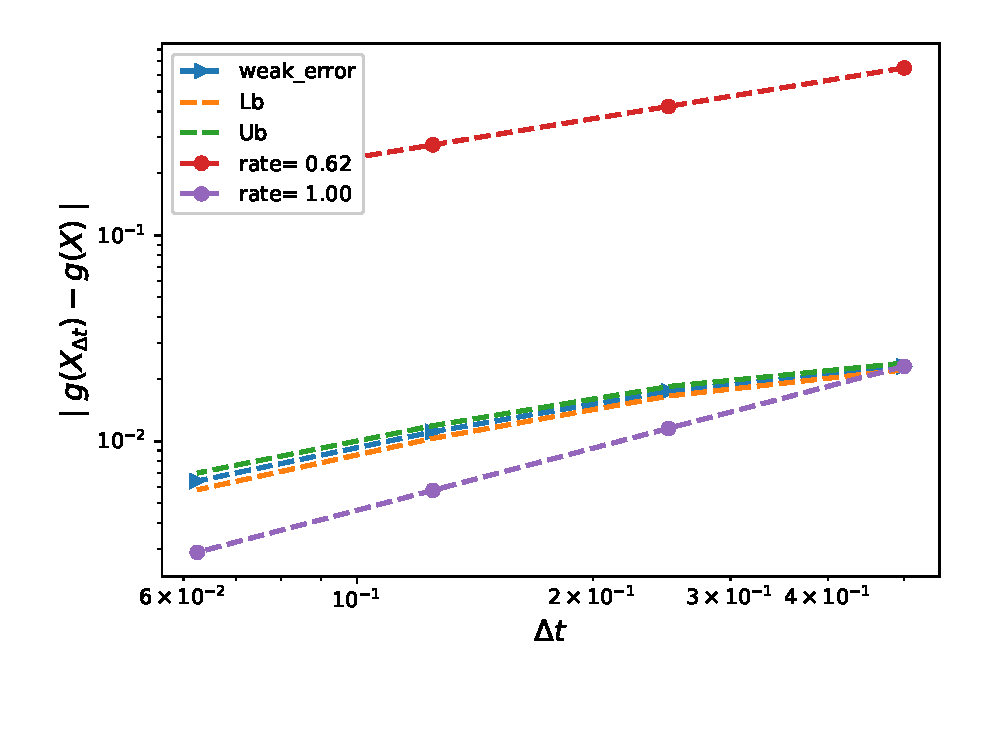
\includegraphics[width=1\linewidth]{./figures/weak_error_rates_call/Beta_10/without_richardson/weak_convergence_order_call_option_relative_M_10_5}
		\caption{}
		\label{fig:sub3}
	\end{subfigure}%
	\begin{subfigure}{.4\textwidth}
		\centering
		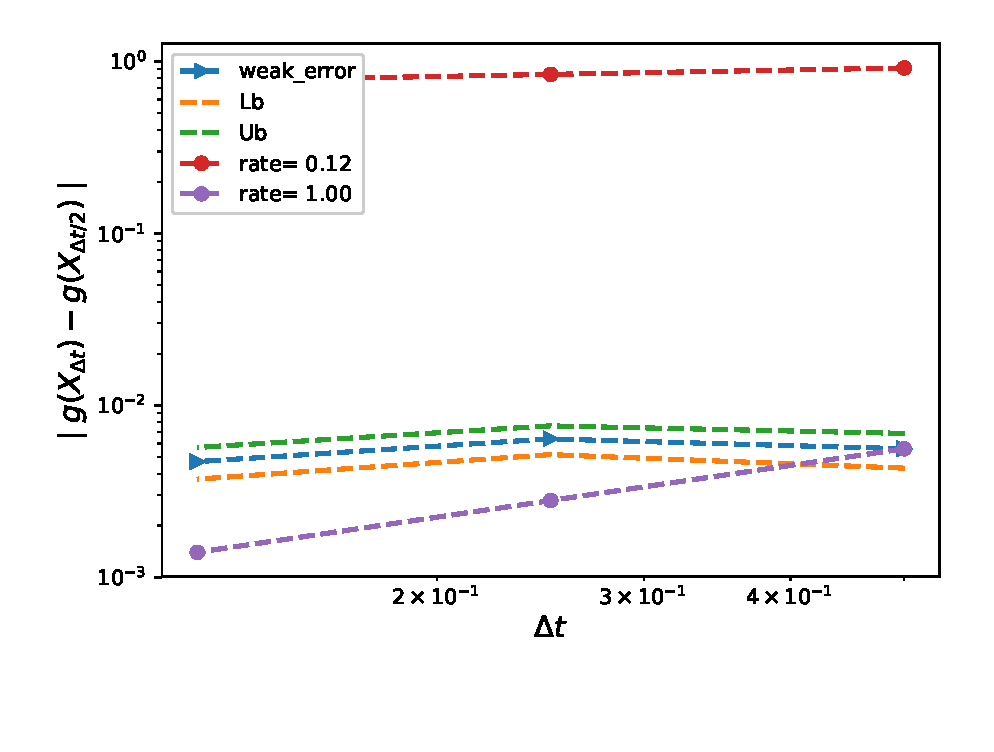
\includegraphics[width=1\linewidth]{./figures/weak_error_rates_call/Beta_10/without_richardson/weak_convergence_order_differences_call_option_relative_M_10_5}
		\caption{}
		\label{fig:sub4}
	\end{subfigure}
	
	\caption{The rate of convergence of the weak error for the call option, without Richardson extraploation, using MC with $M=10^5$: a) $\abs{\expt{g(X_{\Delta t})}-g(X)}$  b) $\abs{\expt{g(X_{\Delta t})-g(X_{\Delta t/2})}}$ }
	\label{fig:Weak_rate_call_without_rich}
\end{figure}
\begin{figure}[h!]
	\centering
	\begin{subfigure}{.4\textwidth}
		\centering
		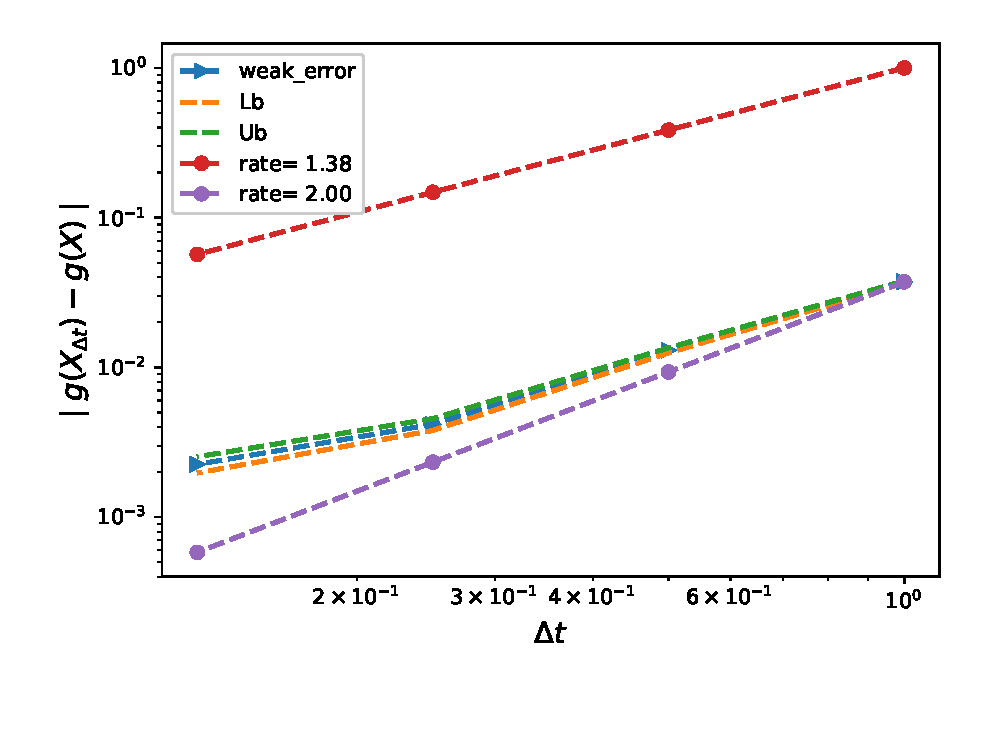
\includegraphics[width=1\linewidth]{./figures/weak_error_rates_call/Beta_10/with_richardson/weak_convergence_order_call_richardson_relative_M_10_6}
		\caption{}
		\label{fig:sub3}
	\end{subfigure}%
	\begin{subfigure}{.4\textwidth}
		\centering
		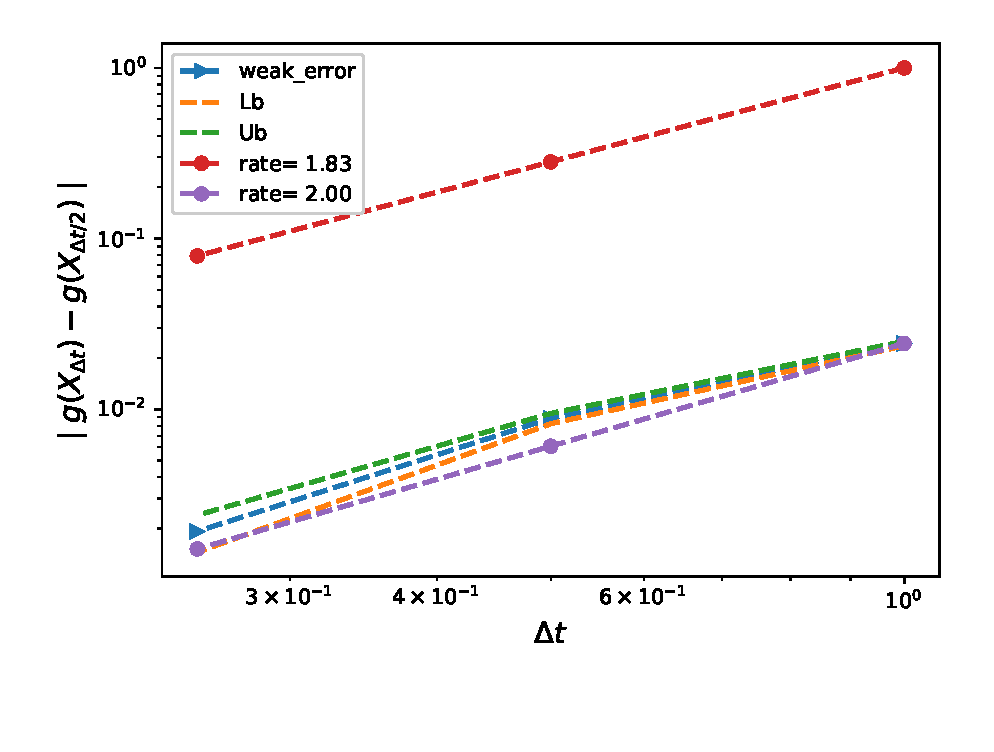
\includegraphics[width=1\linewidth]{./figures/weak_error_rates_call/Beta_10/with_richardson/weak_convergence_order_differences_call_richardson_relative_M_10_6}
		\caption{}
		\label{fig:sub4}
	\end{subfigure}
	
	\caption{The rate of convergence of the weak error for the  call option with Richardson extraploation, using MC with $M=10^6$: a) $\abs{\expt{2 g(X_{\Delta t/2}) -g(X_{\Delta t})}-g(X)}$  b) $\abs{\expt{3 g(X_{\Delta t/2})-g(X_{\Delta t})-2 g(X_{\Delta t/4})}}$ }
	\label{fig:fig:Weak_rate_call_with_rich}
\end{figure}



%\begin{figure}[h!]
%	\centering
%	\begin{subfigure}{.4\textwidth}
%		\centering
%		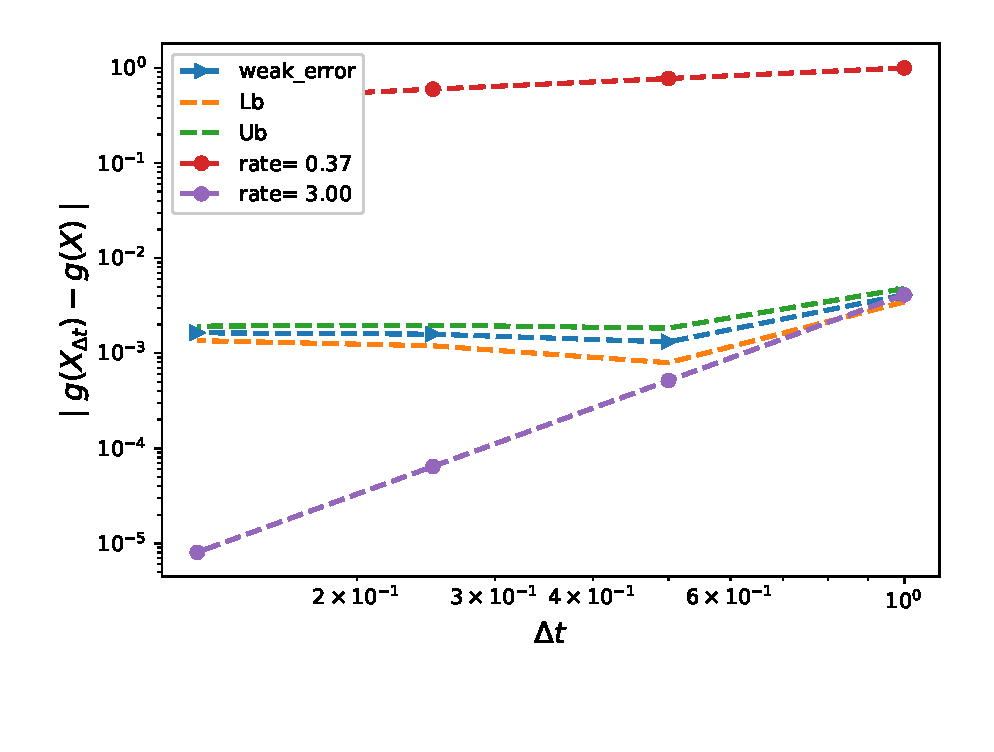
\includegraphics[width=1\linewidth]{./figures/weak_error_rates_call/Beta_10/with_richardson/weak_convergence_order_Call_richardson_level2_relative_M_10_6}
%		\caption{}
%		\label{fig:sub3}
%	\end{subfigure}%
%	\begin{subfigure}{.4\textwidth}
%		\centering
%		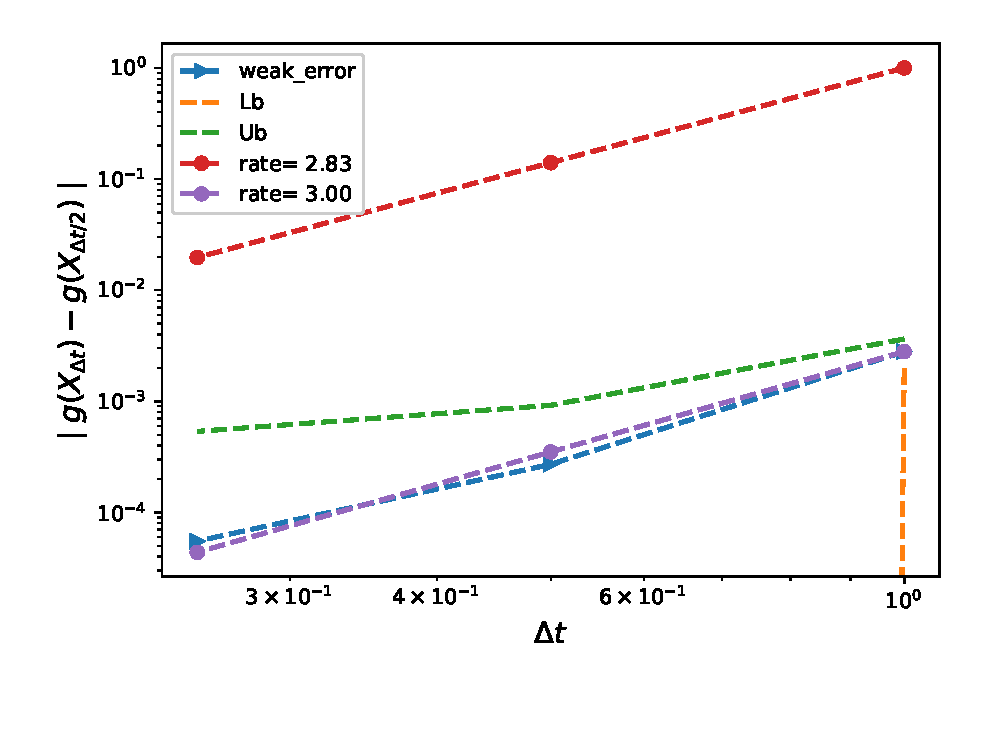
\includegraphics[width=1\linewidth]{./figures/weak_error_rates_call/Beta_10/with_richardson/weak_convergence_order_differences_Call_richardson_level2_relative_M_10_6}
%		\caption{}
%		\label{fig:sub4}
%	\end{subfigure}
	
%	\caption{The rate of convergence of the weak error for the  call option with Richardson extraploation (level 2), using MC with $M=10^6$: a) $\abs{\frac{1}{3}\expt{8 g(X_{\Delta t/4}) -6g(X_{\Delta t/2}) +g(X_{\Delta t})}-g(X)}$  b) $\abs{\frac{1}{3}\expt{-8 g(X_{\Delta t/8}) +14g(X_{\Delta t/4})-7 (X_{\Delta t/2}) +g(X_{\Delta t})}}$}
%	\label{fig:Weak_rate_call_with_rich_level2}
%\end{figure}


\FloatBarrier
\subsubsection*{$\beta=32$}

\begin{figure}[h!]
	\centering
	\begin{subfigure}{.4\textwidth}
		\centering
		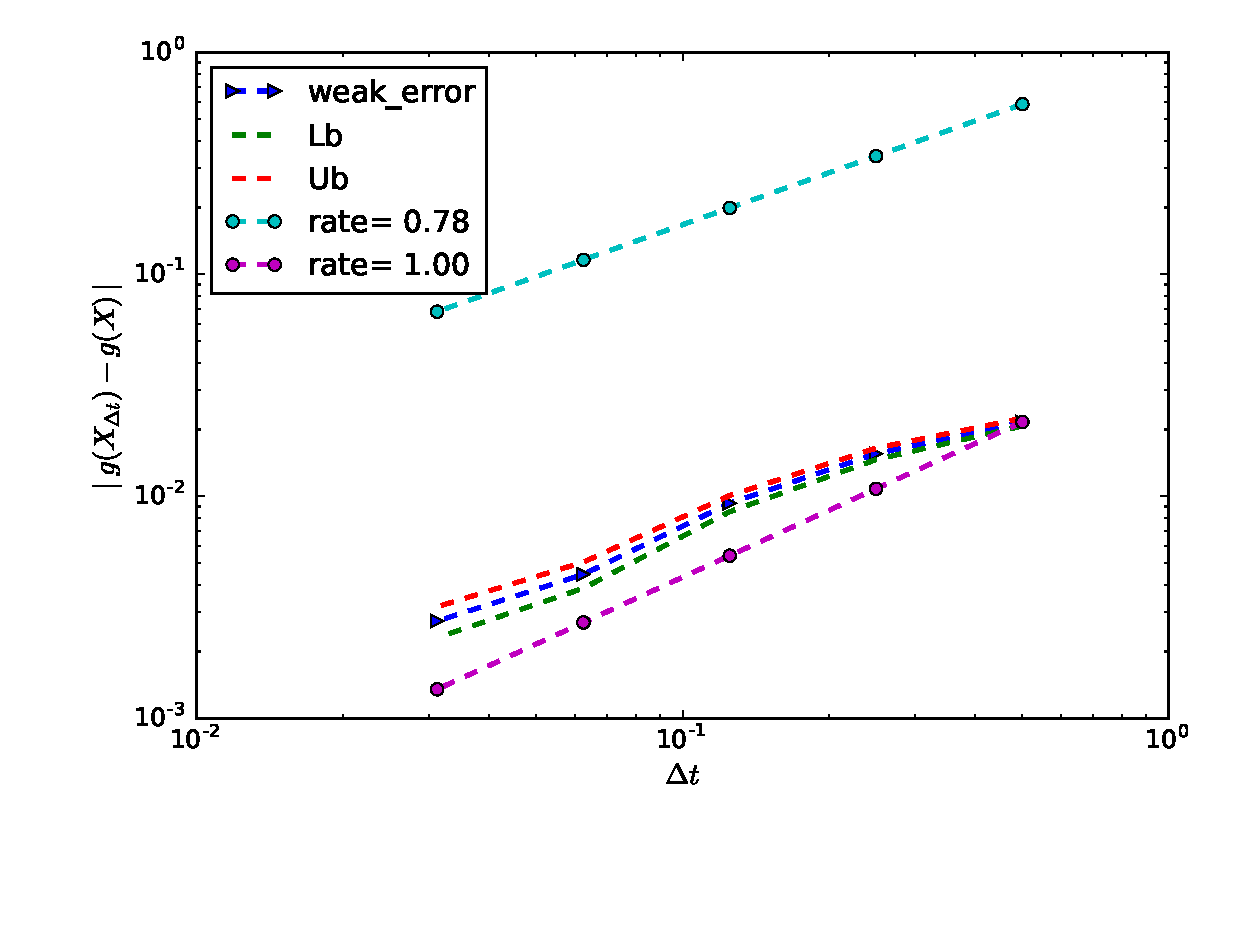
\includegraphics[width=1\linewidth]{./figures/weak_error_rates_call/Beta_32/without_rich/weak_convergence_order_call_option_relative_M_10_5}
		\caption{}
		\label{fig:sub3}
	\end{subfigure}%
	\begin{subfigure}{.4\textwidth}
		\centering
		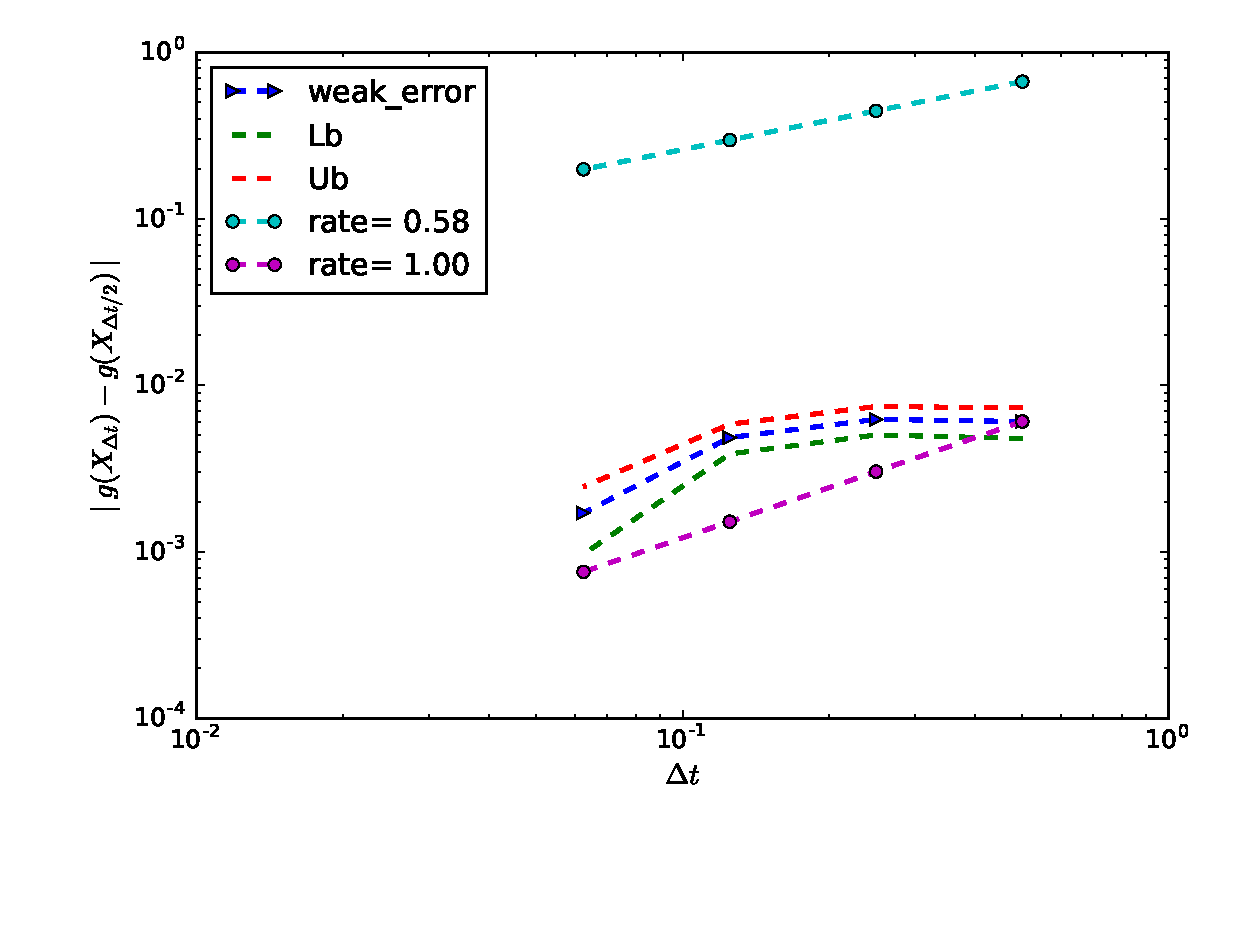
\includegraphics[width=1\linewidth]{./figures/weak_error_rates_call/Beta_32/without_rich/weak_convergence_order_differences_call_option_relative_M_10_5}
		\caption{}
		\label{fig:sub4}
	\end{subfigure}
	
	\caption{The rate of convergence of the weak error for the call option, without Richardson extraploation, using MC with $M=10^5$: a) $\abs{\expt{g(X_{\Delta t})}-g(X)}$  b) $\abs{\expt{g(X_{\Delta t})-g(X_{\Delta t/2})}}$ }
	\label{fig:Weak_rate_call_without_rich_beta_32}
\end{figure}

\begin{figure}[h!]
	\centering
	\begin{subfigure}{.4\textwidth}
		\centering
		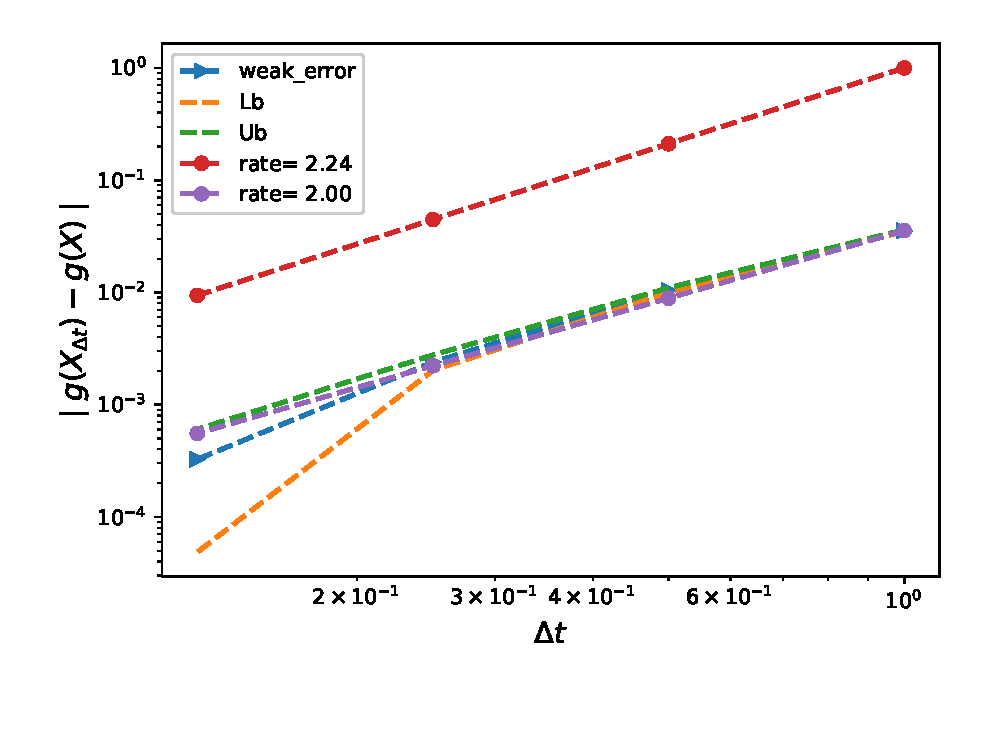
\includegraphics[width=1\linewidth]{./figures/weak_error_rates_call/Beta_32/with_rich/weak_convergence_order_call_richardson_relative}
		\caption{}
		\label{fig:sub3}
	\end{subfigure}%
	\begin{subfigure}{.4\textwidth}
		\centering
		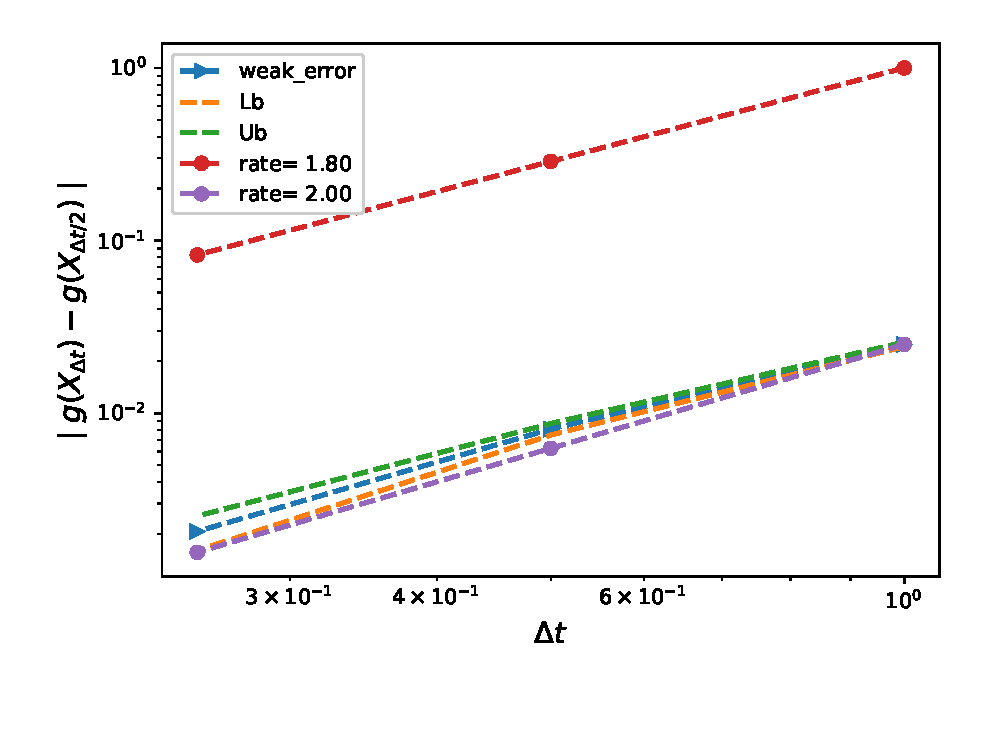
\includegraphics[width=1\linewidth]{./figures/weak_error_rates_call/Beta_32/with_rich/weak_convergence_order_differences_call_richardson_relative}
		\caption{}
		\label{fig:sub4}
	\end{subfigure}
	
	\caption{The rate of convergence of the weak error for the  call option with Richardson extraploation (level 1), using MC with $M=5.10^6$: a) $\abs{\expt{2 g(X_{\Delta t/2}) -g(X_{\Delta t})}-g(X)}$  b) $\abs{\expt{3 g(X_{\Delta t/2})-g(X_{\Delta t})-2 g(X_{\Delta t/4})}}$}
	\label{fig:Weak_rate_call_with_rich_level1_beta_32}
\end{figure}


%\begin{figure}[h!]
%	\centering
%	\begin{subfigure}{.4\textwidth}
%		\centering
%		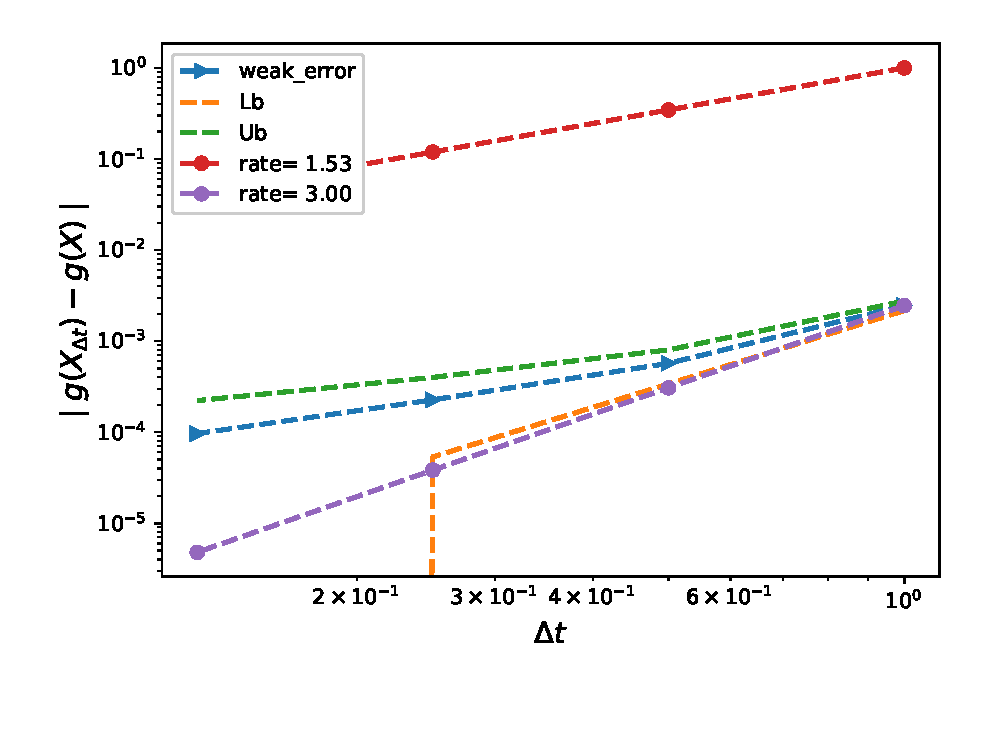
\includegraphics[width=1\linewidth]{./figures/weak_error_rates_call/Beta_32/with_rich/weak_convergence_order_Call_richardson_level2_relative_M_5_10_6}
%		\caption{}
%		\label{fig:sub3}
%	\end{subfigure}%
%	\begin{subfigure}{.4\textwidth}
%		\centering
%		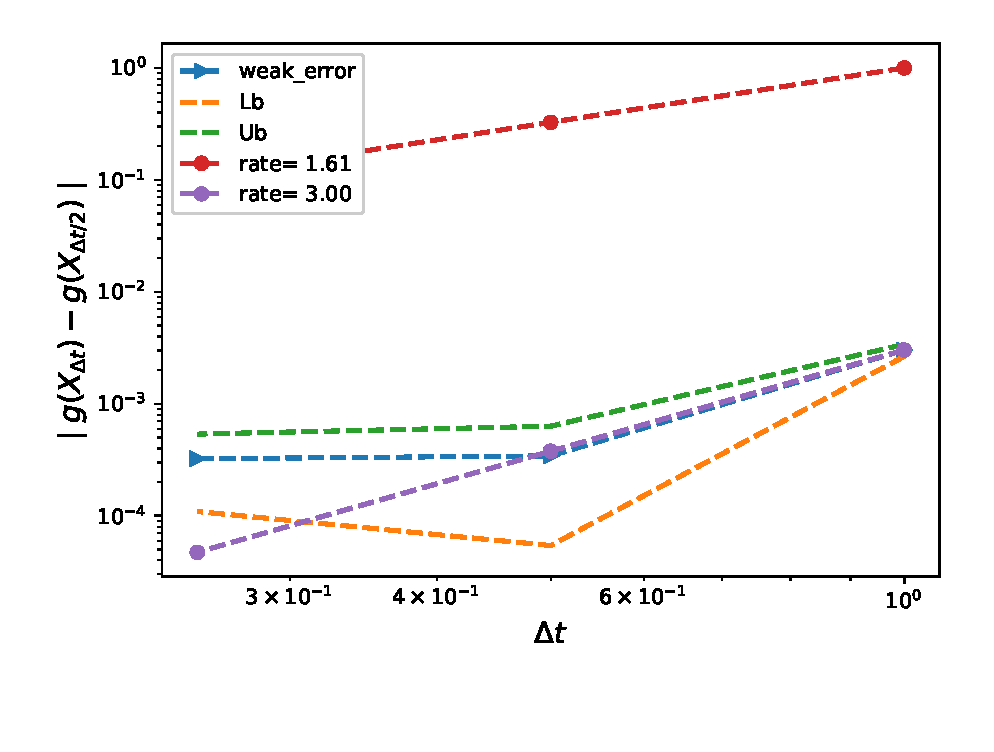
\includegraphics[width=1\linewidth]{./figures/weak_error_rates_call/Beta_32/with_rich/weak_convergence_order_differences_Call_richardson_level2_relative_M_5_10_6}
%		\caption{}
%		\label{fig:sub4}
%	\end{subfigure}
%	
%	\caption{The rate of convergence of the weak error for the  call option with Richardson extraploation (level 2), using MC with $M=5.10^6$: a) $\abs{\frac{1}{3}\expt{8 g(X_{\Delta t/4}) -6g(X_{\Delta t/2}) +g(X_{\Delta t})}-g(X)}$  b) $\abs{\frac{1}{3}\expt{-8 g(X_{\Delta t/8}) +14g(X_{\Delta t/4})-7 (X_{\Delta t/2}) +g(X_{\Delta t})}}$}
%	\label{fig:Weak_rate_call_with_rich_level2_beta_32}
%\end{figure}

\FloatBarrier
\subsubsection{Comparing relative errors}\label{sec:Comparing relative errors, call}
\subsubsection*{Without Richardson extrapolation}



In this Section, we report the results for the Call option, using the different Methods: MISC, MC $+$ root finding  and MC, without Richardson extrapolation . We mention that for MISC we used a very small tolerance for the Newton solver, when solving the Kink point problem ($TOL_{\text{Newton}}=10^{-10}$), we also used $\beta=32$ (number of Laguerre quadrature points ). We start by reporting the observed approximated values using different methods (See table \ref{table:Call option price of the different methods for different number of time steps, without Richardson extrapolation.}). The biased values for MC method were computed using the values of Bias, reported in table \ref{Bias and Statistical errors of MC  for computing Call option price  for different number of time steps, without Richardson extrapolation. The numbers between parentheses are the corresponding absolute errors.}. In table \ref{Quadrature error of MISC to compute Call option price of the different tolerances for different number of time steps, without Richardson extrapolation. The numbers between parentheses are the corresponding absolute errors.}, we report the behavior of quadrature error with respect to MISC tolerance. We precise that the quadrature error is computed by substracting the MISC approximated value from the biased MC value. We report in red the values where MISC becomes stable (see also figure \ref{fig:Quadrature_error_non_rich_Call}). Those values where used to compute the needed number of samples for MC (with and without root finding), to achieve similar magnitude  for statistical error. Later, in table \ref{Total error of MISC and MC to compute Call option price of the different tolerances for different number of time steps, without Richardson extrapolation. The numbers between parentheses are the corresponding absolute errors.}, we report the total relative error for all methods (Quadrature error + Bias for MISC and Statistical error + Bias for MC). We also report in table \ref{Comparsion of the computational time of  MC and MISC, used to compute Call option price  for different number of time steps, without Richardson extrapolation}, the computational time needed for all different methods.  We finally provide in figure \ref{fig:Complexity plot for MC and MISC , Call non rich}, the complexity rates for the different involved methods.

\begin{table}[h!]
	\centering
	\begin{tabular}{l*{6}{c}r}
		Method \textbackslash  Steps            & $2$ & $4$ & $8$ & $16$ &   \\
		\hline
		MISC ($TOl=5.10^{-1},\beta=32$)  & $16.184$ & $16.070$ & $15.998$ & $15.930$  \\
		MISC ($TOl=10^{-1},\beta=32$)  & $16.184$ & $16.070$ & $15.996$ &$15.928$  \\
		MISC ($TOl=5.10^{-2},\beta=32$) & $16.184$ & $16.070$ & $15.996$ & $15.928$  \\
		MISC ($TOl=10^{-2},\beta=32$) & $16.184$ & $16.103$ & $15.996$ &$15.928$  \\
		MISC ($TOl=10^{-3},\beta=32$) & $16.184$ & $16.103$ & $15.996$ & $-$  \\
		
		\hline
		MC method ($M=10^{5}$)   & $  16.194$ & $ 16.099$ & $
		15.999$ & $  15.923$  \\
		\hline
	\end{tabular}
	\caption{Call option price of the different methods for different number of time steps, without Richardson extrapolation.}
	\label{table:Call option price of the different methods for different number of time steps, without Richardson extrapolation.}
\end{table}


\begin{table}[h!]
	\centering
	\begin{tabular}{l*{6}{c}r}
		Method \textbackslash  Steps            & $2$ & $4$ & $8$ & $16$  \\
		\hline
		MC Bias ($M=10^{5}$)  & 	$ \underset{(      0.3424 )}{\mathbf{0.0216}}$  & $\underset{(0.2473)}{\mathbf{ 0.0156
		}}$  & $\underset{(  0.1474)}{\mathbf{0.0093}}$ & $\underset{(     0.0713
	)}{\mathbf{  0.0045 }}$\\ 
		
		MC Statistical error  ($M=10^{5}$)   & 	$ \underset{( 7.5e-03  )}{\mathbf{4.4e-04}}$  & $\underset{(7.5e-03 )}{\mathbf{ 4.7e-04
		}}$  & $\underset{(6.3e-03 )}{\mathbf{4.0e-04}}$ & $\underset{( 4.9e-03 )}{\mathbf{ 3.1e-04  }}$\\ 
	
%		MC Statistical error ($M=10^4$)     & 	$ \underset{( 2.2e-02  )}{\mathbf{1.4e-03}}$  & 	$ \underset{( 2.2e-02  )}{\mathbf{1.4e-03}}$  & $\underset{(1.9e-02 )}{\mathbf{1.2e-03}}$ & $\underset{( 1.5e-02 )}{\mathbf{ 9.3e-04  }}$\\ 
%		
		\hline
	\end{tabular}
	\caption{Bias and Statistical errors of MC  for computing Call option price  for different number of time steps, without Richardson extrapolation. The numbers between parentheses are the corresponding absolute errors.}
	\label{Bias and Statistical errors of MC  for computing Call option price  for different number of time steps, without Richardson extrapolation. The numbers between parentheses are the corresponding absolute errors.}
\end{table}




\begin{table}[h!]
	\centering
	\begin{tabular}{l*{6}{c}r}
		Method \textbackslash  Steps            & $2$ & $4$ & $8$ & $16$  \\
		\hline
		MISC ($TOl=5.10^{-1}$)  & $\underset{( 0.0103)}{\mathbf{\red{0.0007}}}$ & $\underset{(0.0290)}{\mathbf{0.0018}}$  & $\underset{(0.0010
			)}{\mathbf{6.3e-05}}$ &$\underset{(   0.0070)}{\mathbf{0.0004}}$ \\
		MISC ($TOl=10^{-1}$)   &  $\underset{( 0.0103)}{\mathbf{0.0007}}$& $\underset{(0.0290)}{\mathbf{0.0018}}$ & $\underset{(
			0.0030
			)}{\mathbf{\red{0.0002}}}$ &$\underset{(0.0020)}{\mathbf{\red{0.0001}}}$ \\
		MISC ($TOl=5.10^{-2}$)  &$\underset{( 0.0103)}{\mathbf{0.0007}}$ & $\underset{(0.0290)}{\mathbf{0.0018}}$  & $\underset{(
			0.0030
			)}{\mathbf{0.0002}}$ &$\underset{(0.0020)}{\mathbf{0.0001}}$ \\
		MISC ($TOl=10^{-2}$)  & $\underset{( 0.0103)}{\mathbf{0.0007}}$ & $\underset{( 0.0040)}{\mathbf{\red{0.0003}}}$  & $\underset{(
			0.0030
			)}{\mathbf{0.0002}}$ &$\underset{(0.0020)}{\mathbf{0.0001}}$ \\
		MISC ($TOl=10^{-3}$)  & $\underset{( 0.0103)}{\mathbf{0.0007}}$  & $\underset{( 0.0040)}{\mathbf{0.0003}}$ & $\underset{(
			0.0030
			)}{\mathbf{0.0002}}$ &$\underset{(-)}{\mathbf{-}}$ \\
		
		\hline
	\end{tabular}
	\caption{Quadrature error of MISC to compute Call option price of the different tolerances for different number of time steps, without Richardson extrapolation. The numbers between parentheses are the corresponding absolute errors.}
	\label{Quadrature error of MISC to compute Call option price of the different tolerances for different number of time steps, without Richardson extrapolation. The numbers between parentheses are the corresponding absolute errors.}
\end{table}


	\begin{figure}[h!]
\centering
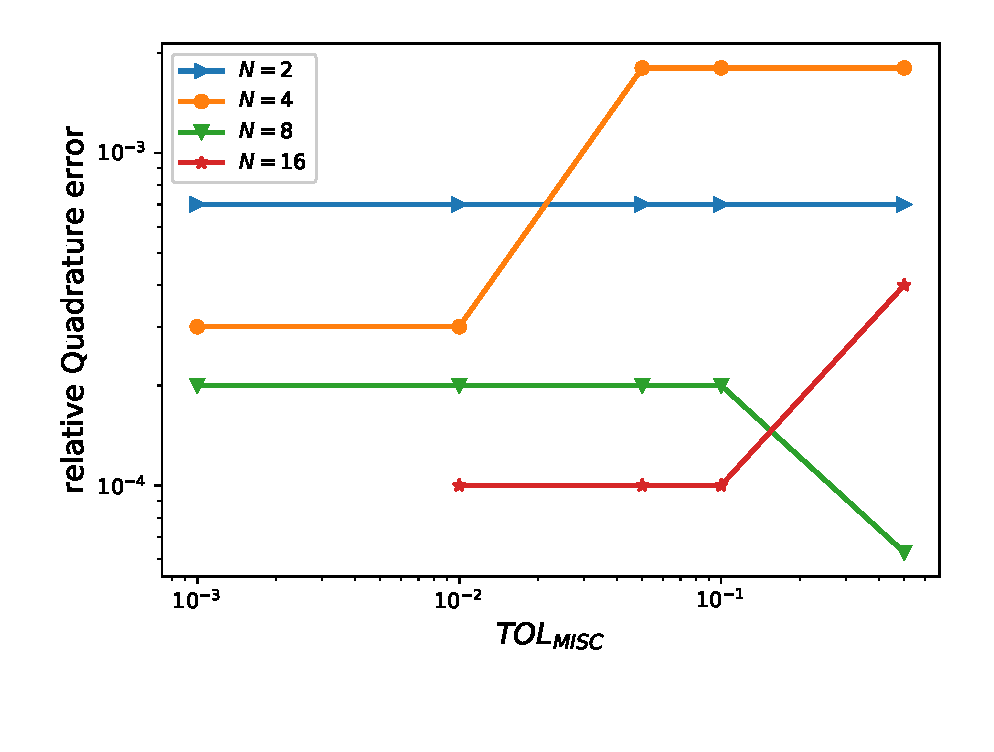
\includegraphics[width=0.7\linewidth]{./figures/Call_MISC_quadrature_error/relative_quad_error_wrt_MISC_TOL_non_rich}


\caption{Relative quadrature error of MISC to compute Call option price of the different tolerances for different number of time steps, without Richardson extrapolation.}
\label{fig:Quadrature_error_non_rich_Call}
\end{figure}



\begin{table}[h!]
	\centering
	\begin{tabular}{l*{6}{c}r}
		Method \textbackslash  Steps            & $2$ & $4$ & $8$ & $16$  \\
		\hline
		MISC ($TOl=5.10^{-1}$)  &  $\mathbf{\red{0.0223}}$ & $\mathbf{0.0174}$ & $\mathbf{0.0094}$ & $\mathbf{0.0049}$  \\
		MISC ($TOl=10^{-1}$)  &  $\mathbf{0.0223}$& $\mathbf{0.0174}$ & $\mathbf{\red{0.0095}}$ & $\mathbf{\red{0.0046}}$  \\
		MISC ($TOl=5.10^{-2}$) & $\mathbf{0.0223}$ & $\mathbf{0.0174}$ &  $\mathbf{0.0095}$ & $\mathbf{0.0046}$  \\
		MISC ($TOl=10^{-2}$)  &  $\mathbf{0.0223}$& $\mathbf{\red{0.0159}}$ & $\mathbf{0.0095}$ &  $\mathbf{0.0046}$  \\
		MISC ($TOl=10^{-3}$) &  $\mathbf{0.0223}$ & $\mathbf{0.0159}$ & $\mathbf{0.0095}$ & $\mathbf{}$  \\
		
		\hline
%		MC  ($M=10^5$)   &  $\mathbf{0.0266}$ & $\mathbf{0.0161}$ & $\mathbf{0.0097}$ & $\mathbf{\red{0.0048}}$  \\	
		
			MC +root finding  &  $\mathbf{\red{0.0223}}$ & $\mathbf{\red{0.0159}}$ & $\mathbf{\red{0.0095}}$ & $\mathbf{\red{0.0046}}$  \\	
				MC   &  $\mathbf{\red{0.0223}}$ & $\mathbf{\red{0.0159}}$ & $\mathbf{\red{0.0095}}$ & $\mathbf{\red{0.0046}}$  \\	
		\hline
	\end{tabular}
	\caption{Total error of MISC and MC to compute Call option price of the different tolerances for different number of time steps, without Richardson extrapolation. The numbers between parentheses are the corresponding absolute errors.}
	\label{Total error of MISC and MC to compute Call option price of the different tolerances for different number of time steps, without Richardson extrapolation. The numbers between parentheses are the corresponding absolute errors.}
\end{table}






\begin{table}[h!]
	\centering
	\begin{tabular}{l*{6}{c}r}
		Method \textbackslash  Steps            & $2$ & $4$ & $8$ & $16$ &   \\
		\hline
		MISC ($TOl=5.10^{-1}$) & $\red{0.3}$ & $3$ & $17$ & $473$  \\
		MISC ($TOl=10^{-1}$)  & $0.3$ & $3$ & $\red{58}$ & $\red{656}$  \\
		MISC ($TOl=5.10^{-2}$)   & $0.3$ & $3$ & $73$ & $731$  \\
		MISC ($TOl=10^{-2}$)  & $0.3$ & $\red{6}$ & $108$ & $1972$  \\
		MISC ($TOl=10^{-3}$)   & $0.3$ & $28$ & $264$ & $-$  \\
		\hline
%		MC method ($M=10^5, \beta=32$)    & $168$ & $216$ & $290$ & $\red{432}$  \\
			MC method +root finding   & $\red{1328}$ & $\red{8140}$ & $\red{21400}$ & $\red{70200}$  \\
				MC method & $\red{1450}$ & $\red{9990}$ & $\red{32790}$ & $\red{ 158108
				}$  \\
		\hline
		
			Ratio of	$\text{(MC+root finding)}/\text{(MISC)}$ & $\red{ 4.4e+03}$ & $\red{   1.4e+03}$ & $\red{369}$ & $\red{ 107}$  \\
		Ratio of	$(\text{MC})/(\text{MISC})$ & $\red{ 4.8e+03}$ & $\red{ 1665}$ & $\red{ 565}$ & $\red{ 241}$  \\
		\hline
	\end{tabular}
	\caption{Comparison of the computational time of  MC and MISC, used to compute Call option price  for different number of time steps, without Richardson extrapolation}
	\label{Comparsion of the computational time of  MC and MISC, used to compute Call option price  for different number of time steps, without Richardson extrapolation}
\end{table}




	\begin{figure}[h!]
\centering
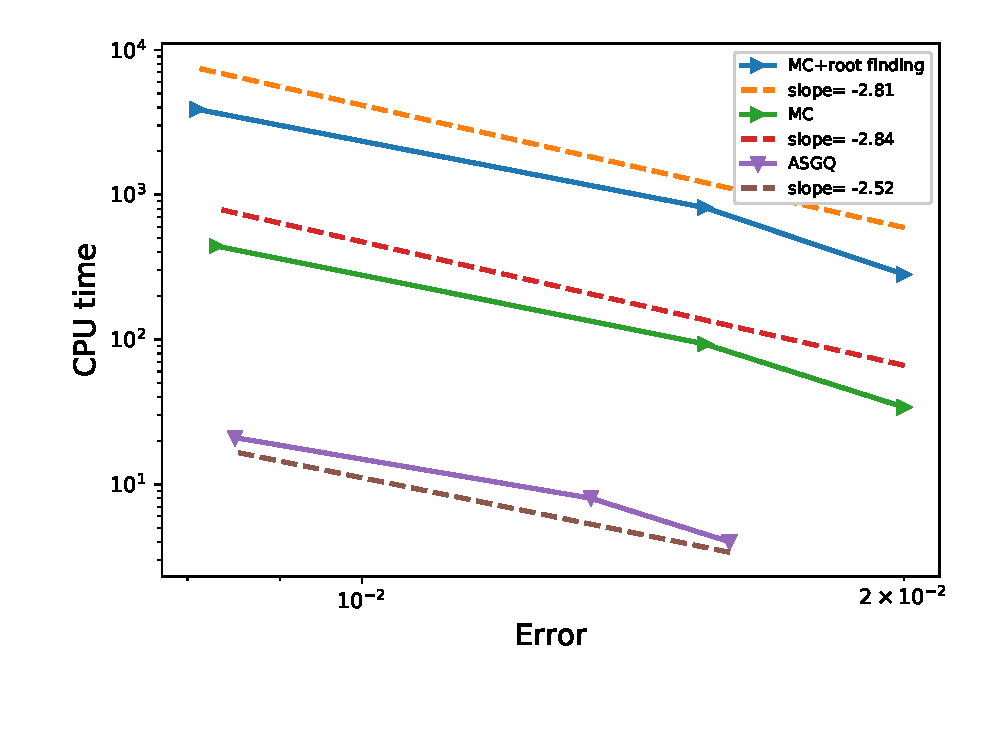
\includegraphics[width=0.7\linewidth]{./figures/Call_Complexity_rates/error_vs_time}

\caption{Complexity plot for MC and MISC for the case without Richardson extrapolation.}
\label{fig:Complexity plot for MC and MISC , Call non rich}
\end{figure}


\FloatBarrier

\subsubsection*{With Richardson extrapolation (level $1$)}




In this Section, we report the results for the Call option, using the different Methods: MISC, MC $+$ root finding  and MC, with Richardson extrapolation . We mention that for MISC we used a very small tolerance for the Newton solver, when solving the Kink point problem ($TOL_{\text{Newton}}=10^{-10}$), we also used $\beta=32$ (number of Laguerre quadrature points ). We start by reporting the observed approximated values using different methods (See table \ref{table: Call option price of the different methods for different number of time steps, with Richardson extrapolation (level1).}. The biased values for MC method were computed using the values of Bias, reported in table \ref{Bias and Statistical errors of MC  for computing Call option price  for different number of time steps, with Richardson extrapolation (level $1$). The numbers between parentheses are the corresponding absolute errors.}. In table \ref{Quadrature error of MISC to compute Call option price of the different tolerances for different number of time steps, with Richardson extrapolation (level $1$). The numbers between parentheses are the corresponding absolute errors.}, we report the behavior of quadrature error with respect to MISC tolerance. We precise that the quadrature error is computed by substracting the MISC approximated value from the biased MC value. We report in red the values where MISC becomes stable (see also figure \ref{fig:Quadrature_error_with_rich_Call}). Those values where used to compute the needed number of samples for MC (with and without root finding), to achieve similar magnitude  for statistical error. Later, in table \ref{Total error of MISC and MC to compute Call option price of the different tolerances for different number of time steps, with Richardson extrapolation (level $1$). The numbers between parentheses are the corresponding absolute errors.}, we report the total relative error for all methods (Quadrature error + Bias for MISC and Statistical error + Bias for MC). We also report in table\ref{Comparsion of the computational time of  MC and MISC, used to compute Call option price  for different number of time steps, with Richardson extrapolation (level $1$)}, the computational time needed for all different methods.  We finally provide in figure \ref{fig:Complexity plot for MC and MISC , Call, comparison}, the comparison between the two versions of MISC (without/with Richardson extrapolation).



\begin{table}[h!]
	\centering
	\begin{tabular}{l*{6}{c}r}
		Method \textbackslash  Steps            & $1-2$ & $2-4$ & $4-8$ & $8-16$ &   \\
		\hline
		MISC ($TOl=5.10^{-1}$)  & $16.4108$ & $16.0254$ & $15.8912$ & $15.8621$  \\
		MISC ($TOl=10^{-1}$)  & $16.4108$ & $16.0254$ & $15.8883$ & $15.8603$  \\
		MISC ($TOl=5.10^{-2}$) & $16.4108$ & $16.0218$ & $15.8885$ & $15.8600$  \\
		MISC ($TOl=10^{-2}$) & $16.4108$& $16.0218$ & $15.8888$ & $15.8595$  \\
		MISC ($TOl=10^{-3}$) & $16.4108$ & $16.0207$ & $15.8885$ & $-$  \\
		
		\hline
		MC method ($M=5.10^{6}$)   & $  16.4147$ & $ 16.0184$ & $15.8900$ & $15.8567$  \\
		\hline
	\end{tabular}
	\caption{Call option price of the different methods for different number of time steps, with Richardson extrapolation (level $1$).}
	\label{table: Call option price of the different methods for different number of time steps, with Richardson extrapolation (level1).}
\end{table}


\begin{table}[h!]
	\centering
	\begin{tabular}{l*{6}{c}r}
		Method \textbackslash  Steps            & $1-2$ & $2-4$ & $4-8$ & $8-16$  \\
		\hline
		MC Bias ($M=5.10^6$)   & 	$ \underset{(    0.5627
			 )}{\mathbf{0.0355}}$  & $\underset{(  0.1664)}{\mathbf{ 0.0105
		}}$  & $\underset{( 0.0380)}{\mathbf{0.0024}}$ & $\underset{( 0.0048
	 )}{\mathbf{ 0.0003  }}$\\ 
		
		MC Statistical error ($M=5.10^6$)     & 	$ \underset{(  4.4e-03 )}{\mathbf{2.8e-04}}$  & $\underset{(3.8e-03 )}{\mathbf{ 2.4e-04
		}}$  & $\underset{(3.0e-03)}{\mathbf{1.9e-04}}$ & $\underset{(2.2e-03 )}{\mathbf{ 1.4e-04  }}$\\ 
		
%			MC Statistical error ($M=10^5$)     & 	$ \underset{(  1.4e-02 )}{\mathbf{9.0e-04}}$  & $\underset{(1.3e-02)}{\mathbf{ 8.0e-04
%		}}$  & $\underset{(9.4e-03)}{\mathbf{5.9e-04}}$ & $\underset{( 7.1e-03 )}{\mathbf{ 4.5e-04  }}$\\ 
		\hline
	\end{tabular}
	\caption{Bias and Statistical errors of MC  for computing Call option price  for different number of time steps, with Richardson extrapolation (level $1$). The numbers between parentheses are the corresponding absolute errors.}
	\label{Bias and Statistical errors of MC  for computing Call option price  for different number of time steps, with Richardson extrapolation (level $1$). The numbers between parentheses are the corresponding absolute errors.}
\end{table}




\begin{table}[h!]
	\centering
	\begin{tabular}{l*{6}{c}r}
		Method \textbackslash  Steps            & $1-2$ & $2-4$ & $4-8$ & $8-16$  \\
		\hline
		MISC ($TOl=5.10^{-1}$)  & $\underset{(0.0039
			)}{\mathbf{ \red{2.5e-04}}}$ & $\underset{(0.0070)}{\mathbf{4.4e-04}}$  & $\underset{(0.0012
			)}{\mathbf{7.6e-05}}$ &$\underset{(0.0054)}{\mathbf{3.4e-04}}$ \\
		MISC ($TOl=10^{-1}$)   & $\underset{(0.0039
			)}{\mathbf{ 2.5e-04}}$ & $\underset{(0.0070)}{\mathbf{4.4e-04}}$  & $\underset{(  0.0017)}{\mathbf{1.1e-04}}$ &$\underset{(0.0036)}{\mathbf{\red{2.3e-04}}}$ \\
		MISC ($TOl=5.10^{-2}$)  & $\underset{(0.0039
			)}{\mathbf{ 2.5e-04}}$ & $\underset{(0.0034)}{\mathbf{\red{\red{2.1e-04}}}}$  & $\underset{(    0.0015)}{\mathbf{\red{9.5e-05}}}$ &$\underset{(0.0033)}{\mathbf{2.1e-04}}$ \\
		MISC ($TOl=10^{-2}$)  & $\underset{(0.0039
			)}{\mathbf{ 2.5e-04}}$ & $\underset{(0.0034)}{\mathbf{2.1e-04}}$  & $\underset{(0.0012
			)}{\mathbf{7.6e-05}}$&$\underset{(0.0028
			)}{\mathbf{1.7e-04}}$ \\
		MISC ($TOl=10^{-3}$)  & $\underset{(0.0039
			)}{\mathbf{ 2.5e-04}}$ & $\underset{(0.0023
			)}{\mathbf{1.5e-04}}$   &$\underset{(    0.0015)}{\mathbf{9.5e-05}}$ & $\underset{()}{\mathbf{}}$ \\
		
		\hline
	\end{tabular}
	\caption{Quadrature error of MISC to compute Call option price of the different tolerances for different number of time steps, with Richardson extrapolation (level $1$). The numbers between parentheses are the corresponding absolute errors.}
	\label{Quadrature error of MISC to compute Call option price of the different tolerances for different number of time steps, with Richardson extrapolation (level $1$). The numbers between parentheses are the corresponding absolute errors.}
\end{table}




	\begin{figure}[h!]
\centering
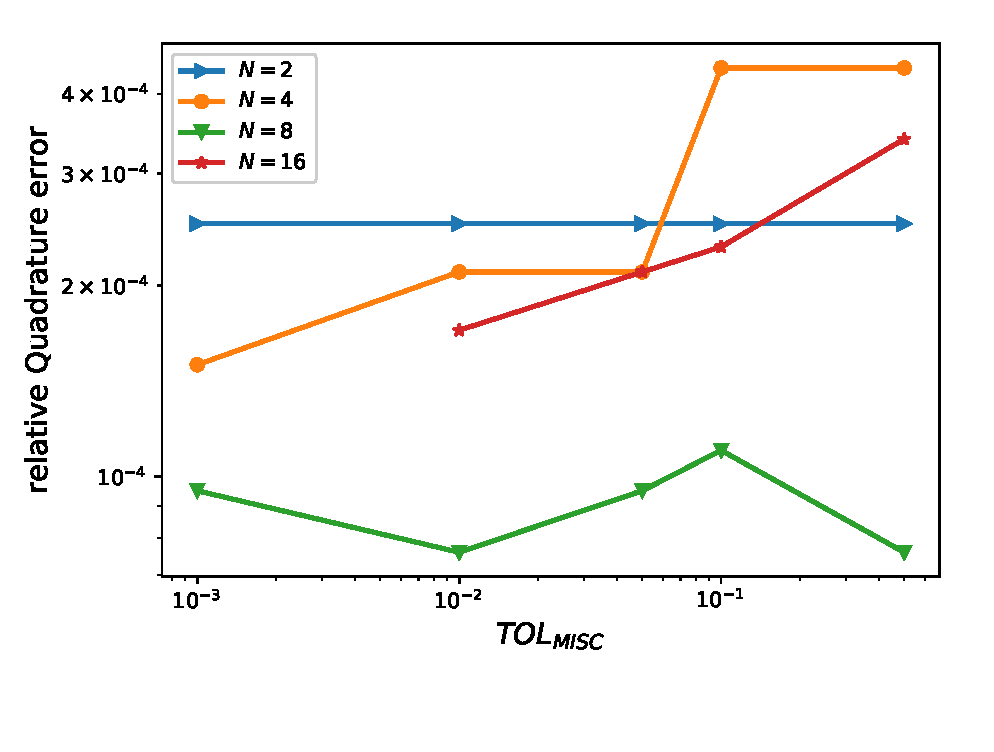
\includegraphics[width=0.7\linewidth]{./figures/Call_MISC_quadrature_error/relative_quad_error_wrt_MISC_TOL_with_rich}


\caption{Relative quadrature error of MISC to compute Call option price of the different tolerances for different number of time steps, with Richardson extrapolation.}
\label{fig:Quadrature_error_with_rich_Call}
\end{figure}





\begin{table}[h!]
	\centering
	\begin{tabular}{l*{6}{c}r}
		Method \textbackslash  Steps            & $1-2$ & $2-4$ & $4-8$ & $8-16$  \\
		\hline
		MISC ($TOl=5.10^{-1}$)  &  $\mathbf{\red{0.0358}}$ & $\mathbf{0.0109}$ & $\mathbf{0.0025}$ & $\mathbf{0.0006}$  \\
		MISC ($TOl=10^{-1}$)  &  $\mathbf{0.0358}$ & $\mathbf{0.0109}$ & $\mathbf{0.0025}$ & $\mathbf{\red{0.0005}}$  \\
		MISC ($TOl=5.10^{-2}$) &  $\mathbf{0.0358}$ & $\mathbf{\red{0.0107}}$ & $\mathbf{\red{0.0025}}$ & $\mathbf{0.0005}$  \\
		MISC ($TOl=10^{-2}$)  &  $\mathbf{0.0358}$ & $\mathbf{0.0107}$ & $\mathbf{0.0025}$ & $\mathbf{0.0005}$ \\
		MISC ($TOl=10^{-3}$) &  $\mathbf{0.0358}$ & $\mathbf{0.0107}$ & $\mathbf{0.0025}$ & $\mathbf{}$  \\
		
		\hline
%		MC  ($M=5.10^6$)   &  $\mathbf{\red{0.0358}}$ & $\mathbf{\red{0.0107}}$ & $\mathbf{\red{0.0026}}$ & $\mathbf{\red{0.0004}}$  \\	
%			MC + root finding  &  $\mathbf{\red{0.0358}}$ & $\mathbf{\red{0.0107}}$ & $\mathbf{\red{0.0025}}$ & $\mathbf{\red{0.}}$  \\	
		\hline
	\end{tabular}
	\caption{Total error of MISC  to compute Call option price of the different tolerances for different number of time steps, with Richardson extrapolation (level $1$). The numbers between parentheses are the corresponding absolute errors.}
	\label{Total error of MISC and MC to compute Call option price of the different tolerances for different number of time steps, with Richardson extrapolation (level $1$). The numbers between parentheses are the corresponding absolute errors.}
\end{table}






\begin{table}[h!]
	\centering
	\begin{tabular}{l*{6}{c}r}
		Method \textbackslash  Steps            & $1-2$ & $2-4$ & $4-8$ & $8-16$ &   \\
		\hline
		MISC ($TOl=5.10^{-1}$) & $\red{0.3}$ & $4$ & $56$ & $713$  \\
		MISC ($TOl=10^{-1}$)  & $0.3$  & $4$ & $107$ & $\red{1126}$  \\
		MISC ($TOl=5.10^{-2}$)   & $0.3$  & $\red{9}$ & $\red{135}$ & $1253$  \\
		MISC ($TOl=10^{-2}$)  &  $0.3$  & $9$ & $186$ & $3540$  \\
		MISC ($TOl=10^{-3}$)   & $0.3$  & $63$ & $836$ & $$  \\
		\hline
%		MC +root finding   & $\red{ 2.4e+05}$ & $\red{ 4.3e+05}$ & $\red{ 3.5e+06}$ & $\red{-}$  \\
		\hline
	\end{tabular}
	\caption{Comparsion of the computational time of  MISC, used to compute Call option price  for different number of time steps, with Richardson extrapolation (level $1$)}
	\label{Comparsion of the computational time of  MC and MISC, used to compute Call option price  for different number of time steps, with Richardson extrapolation (level $1$)}
\end{table}

%	\begin{figure}[h!]
%	\centering
%	\includegraphics[width=0.7\linewidth]{./figures/Call_Complexity_rates/error_vs_time_rich}
%	
%	\caption{Complexity plot for MC and MISC for the case with Richardson extrapolation.}
%	\label{fig:Complexity plot for MC and MISC , Call, with rich}
%\end{figure}







\begin{figure}[h!]
	\centering
	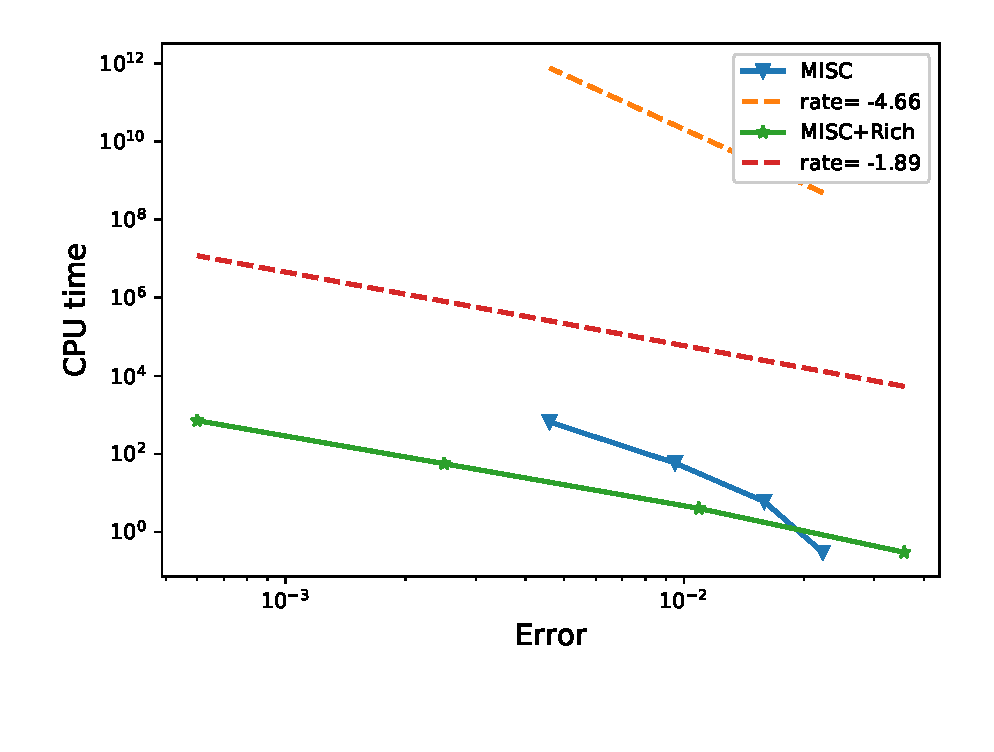
\includegraphics[width=0.7\linewidth]{./figures/Call_Complexity_rates/error_vs_time_comparision}
	
	\caption{Complexity plot for MISC without and with Richardson extrapolation, for the Call option.}
	\label{fig:Complexity plot for MC and MISC , Call, comparison}
\end{figure}




\FloatBarrier
%In the following, we compare the  relative errors for the call option example under Black-Scholes model(see Tables (\ref{Relative error of the call option price of the different tolerances for different number of time steps.}, \ref{Relative error of Call option price of the different tolerances for different number of time steps, using Richardson extrapolation (level $1$)}, \ref{Relative error of Call option price of the different tolerances for different number of time steps, using Richardson extrapolation (level $2$)})). We report the results for $3$ scenarios: i) Without using Richardson extrapolation, ii) Using level $1$ Richardson extrapoaltion, iii) Using level $2$ Richardson extrapoaltion.  You may see appendix \ref{appendix:Call prices for different methods} for the values of call option prices. The value of $\beta$ used to get those points is $\beta=10$.
%
%Given the normalized bias computed by MC method (See Section \ref{sec:Weak error plots_call}) (reported as bold values in the tables), we report in red in each table the smallest tolerance that MISC required to get below that relative bias (I do not put values for smaller tolerances, once the required bias is reached). In case I do not reach those bias I put the best value that I get with MISC in red.
%
%From the tables (\ref{Relative error of the call option price of the different tolerances for different number of time steps.}, \ref{Relative error of Call option price of the different tolerances for different number of time steps, using Richardson extrapolation (level $1$)}, \ref{Relative error of Call option price of the different tolerances for different number of time steps, using Richardson extrapolation (level $2$)})), we may observe that to get a relative error below $0.5\%$, we need more than $16$ time steps for the case without Richardson extrapolation compared to only using $4$ time step in the coarse level for the case of level $1$ Richardson extraplation,  and  only using $1$ time step in the coarse level for the case of level $2$ Richardson extraplation.

%\begin{table}[h!]
%	\centering
%	\begin{tabular}{l*{6}{c}r}
%		Method \textbackslash  Steps            & $2$ & $4$ & $8$ & $16$ &   \\
%		\hline
%		MISC ($TOl=5.10^{-1}$)  & $ \red{0.0229}$ & $  0.0179$ & $\red{0.0111}$ & $ 0.0068$  \\
%		MISC ($TOl=10^{-3}$)  & $-$ & $ \red{ 0.0177}$ & $-$ & $\red{  0.0066}$  \\
%			MC method ($M=10^{5}$)&$ \mathbf{0.0231}$    & $\mathbf{0.0175}$  & $\mathbf{0.0111}$  & $\mathbf{0.0064}$ \\	
%		\hline
%	\end{tabular}
%	\caption{Relative error of the call option price of the different tolerances for different number of time steps, without Richardson extrapolation}
%	\label{Relative error of the call option price of the different tolerances for different number of time steps.}
%\end{table}

%\begin{table}[h!]
%	\centering
%	\begin{tabular}{l*{5}{c}r}
%		Method \textbackslash  Steps    &$1-2$        & $2-4$ & $4-8$ & $8-16$  \\
%		\hline
%		MISC ($TOl=5.10^{-1}$)  &$\red{0.0372}$ & $ 0.0129$ & $0.0043$ & $ 0.0025$  \\
%		MISC ($TOl=10^{-3}$) & $-$ & $ \red{0.0126}$ & $\red{    0.0042}$ & $\red{0.0023}$   \\
%		MC method ($M=10^{5}$)&$ \mathbf{0.0374}$    & $\mathbf{0.0116}$  & $\mathbf{0.0027}$  & $\mathbf{0.0022}$ \\
%		\hline
%	\end{tabular}
%	\caption{Relative error of the call option price of the different tolerances for different number of time steps, using Richardson extrapolation (level $1$)}
%	\label{Relative error of Call option price of the different tolerances for different number of time steps, using Richardson extrapolation (level $1$)}
%\end{table}


%\begin{table}[h!]
%	\centering
%	\begin{tabular}{l*{5}{c}r}
%		Method \textbackslash  Steps    &$1-2-4$        & $2-4-8$ & $4-8-16$   \\
%		\hline
%		MISC ($TOl=5.10^{-1}$)  &$0.0047$ & $  0.0015$ & $0.0019
%		$   \\
%		MISC ($TOl=10^{-3}$) & $ \red{0.0043}$ & $ \red{0.0013}$ & $\red{  0.0017}$    \\
%		MC method ($M=10^{6}$)&$ \mathbf{0.0041}$    & $\mathbf{0.0013}$  & $\mathbf{0.0016}$  \\
%		\hline
%	\end{tabular}
%	\caption{Relative error of the call option price of the different tolerances for different number of time steps, using Richardson extrapolation (level $2$)}
%	\label{Relative error of Call option price of the different tolerances for different number of time steps, using Richardson extrapolation (level $2$)}
%\end{table}
\FloatBarrier





%\section{TO-DO}
%
%\begin{enumerate}
%	\item Carrying out the Richardson extrapolation in the non-smooth
%	case.
%\end{enumerate}
%\subsection{CIR process}
%
%The impact of the Brownian bridge will disappear in the limit, which may make the effect of the smoothing, but also of the errors in the kink location difficult to identify (This observation is not clear to me yet). For this reason, we study a more complicated 1-dimensional problem. In fact, we use a CIR process. To avoid complications at the boundary, we use nice parameter choices, such that the discretized process is very unlikely to hit the boundary (Feller condition).
%
%
%
%The CIR model specifies that the instantaneous interest rate follows the SDE given by
%\begin{equation}\label{CIR_process}
%dX_t=a(b-X_t)dt+\sigma \sqrt{X_t} dW_t,\: X(0)=X_0>0
%\end{equation}
%where and $a>0$, $b>0$ and $\sigma>0$, are the parameters. The parameter $a$ corresponds to the speed of adjustment, $b$ to the mean and $\sigma$ to volatility. 
%
%If the parameters obey the following condition (known as the Feller condition) then the process $X_t$  is strictly positive
%\begin{equation}\label{Feller_condition}
%2 a b \geq\sigma^2.
%\end{equation}
%
%The SDE \eqref{CIR_process} is not explicitly solvable. In general there are two ways to do it, namely, exact simulation methods and approximation schemes. Exact simulation in general requires more time
%than a simulation with approximation schemes (Up to a factor 10). Therefore, it is used to compute expectations that depend on the values of the process at just a few fixed times. However, for expectations that depends on all the path (such as integrals) discretization schemes should be preferred. 
%
%The main problem  when discretizing a CIR process using Euler scheme is that it can lead to negative values for which the square root is not defined. In fact, if we consider the following straightforward Euler scheme on the time interval $[0,T]$ for a CIR process $X(t)$:
%\begin{equation}\label{Euler_CIR}
%\bar{X}(t_{i+1})=\bar{X}(t_i)+a(b-\bar{X}(t_i)) \Delta t_i+\sigma \sqrt{\bar{X}(t_i)} \Delta W_i,
%\end{equation}
%
%then it can lead to negative values since the Gaussian
%increment is not bounded from below. Thus, this  scheme is not well defined.
%
%Many modified Euler schemes were proposed to overcome this issue. For instance, Deelstra and Delbaen \cite{deelstra1998convergence} have propose the full truncation scheme given by
%\begin{equation}\label{Full_truncation_CIR}
%\bar{X}(t_{i+1})=\bar{X}(t_i)+a(b-\bar{X}(t_i)) \Delta t_i+\sigma \sqrt{\bar{X}(t_i)^+} \Delta W_i.
%\end{equation}
%
%Higham and Mao \cite{mao2007stochastic} proposed the following scheme
% \begin{equation}\label{partial_reflection_CIR}
% \bar{X}(t_{i+1})=\bar{X}(t_i)+a(b-\bar{X}(t_i)) \Delta t_i+\sigma \sqrt{\abs{\bar{X}(t_i)}} \Delta W_i.
% \end{equation}
% Lord et al \cite{lord2010comparison} proposed the following scheme
% 
% \begin{equation}\label{truncation_CIR}
% \bar{X}(t_{i+1})=\bar{X}(t_i)+a(b-\bar{X}(t_i)^+) \Delta t_i+\sigma \sqrt{\bar{X}(t_i)^+} \Delta W_i.
% \end{equation}
% 
% 
%Diop proposed in \cite{berkaoui2008euler} proposed the reflection scheme, given by
%\begin{equation}\label{Reflection_CIR}
%\bar{X}(t_{i+1})=\mid\bar{X}(t_i)+a(b-\bar{X}(t_i)) \Delta t_i+\sigma \sqrt{\bar{X}(t_i)} \Delta W_i \mid.
%\end{equation}
%Also, implicit and higher order schemes were proposed by Alfonsi \cite{alfonsi2005discretization,alfonsi2008second,alfonsi2010high}.
%
%Those modified Euler schemes were studied  numerically in \cite{alfonsi2005discretization}. It is observed that when $\sigma$ is small enough, typically $\sigma^2 \le 2a$, these schemes have a weak error of order one and a strong error of order $1/2$. However, when $\sigma$ is getting large, say $\sigma^2\gg 4a$, the convergence of all these schemes is degraded. As observed
%by Lord et al. \cite{lord2010comparison}, the schemes \eqref{Full_truncation_CIR} and \eqref{truncation_CIR} behave better than the schemes \eqref{partial_reflection_CIR} and \eqref{Reflection_CIR}. In fact, when $\sigma$ gets large, the CIR process spends more time close to zero and get stuck in the neighbourhood of zero when $\sigma$ is really large. When the scheme takes a negative value, the absolute value in  both schemes (\eqref{partial_reflection_CIR},\eqref{Reflection_CIR}) produces a noise that pushes the scheme away from zero. On the other hand, the positive part in truncation schemes cancels the noise when the scheme gets negative, which better reproduces the behaviour of the
%CIR process. 
%
%In the following, we use the scheme given by \eqref{Full_truncation_CIR} to simulate the discrete CIR process.
%\subsubsection{Location of the kink for the discrete problem: Using full truncation scheme}\label{sec:kink_location_full_truncation)_CIR}
%
%
%The full truncation scheme simulating the CIR process is given by \eqref{Full_truncation_CIR}. Here we are interested in finding the location of the kink for hockey-stick function.
%
%
%Using Brownian bridge construction given by \eqref{Brownian_bridge}, we have
%\begin{align}\label{recursion_full_truncation_CIR}
%X_{t_1}&= X_{t_0} \left[ 1- a \Delta t  \right]+ \sigma \sqrt{X_{t_0}^+} \left[   Y \frac{\Delta t}{\sqrt{T}} + \Delta B_0\right]+ ab \Delta t\nonumber\\
%X_{t_2}&= X_{t_1} \left[ 1- a \Delta t  \right]+ \sigma \sqrt{X_{t_1}^+} \left[   Y \frac{\Delta t}{\sqrt{T}} + \Delta B_1\right]+ ab \Delta t \nonumber\\ 
%\vdots &= \vdots =\vdots \nonumber\\
%X_{t_N}&= X_{t_{N-1}} \left[ 1- a \Delta t  \right]+ \sigma \sqrt{X_{t_{N-1}}^+} \left[   Y \frac{\Delta t}{\sqrt{T}} + \Delta B_{N-1} \right]+ ab \Delta t ,
%\end{align}
%
%
%to simplify the notation we set $f_i(y):=X_{t_i}$. Then  the location of the kink point for the approximate problem is equivalent to finding the roots of the polynomial $P(y_\ast(K))$, given by
%\begin{align}\label{polynomial_kink_location_CIR_full_truncation}
%P(y_{\ast}(K))=f_N(y_\ast(K))-\frac{K}{X_0},
%\end{align}
%where $f_N(y)$ is computed using recursion \eqref{recursion_full_truncation_CIR}.
%
%To apply the \textbf{Newton iteration method}, we need the derivative $P'=\frac{d P}{d y_\ast}=f_N'$, which is deduced from recursion \eqref{recursion_full_truncation_CIR}, and given by the the following relation
%\begin{align}
%f_i'(y) &= f_{i-1}'(y)\left[1-a \Delta t \right]+ \sigma \sqrt{f_{i-1}(y)^+} \left[ \frac{\Delta t}{\sqrt{T}}+ \left[y \frac{\Delta t}{\sqrt{T}}+\Delta B_{i-1}\right] \frac{f_{i-1}'(y)}{2} \right],\: 1 \le i \le N \nonumber\\
%f_0'&=0.
%\end{align}
%
%
%
%
%\subsubsection{Results}
%The code of this section is found in the script discretized\_CIR.py, which compares the different ways of determining the kink location for 1D CIR model.
%









 %%%%%%%%%%%%%%%%%%%%%%%%%%%%%%%%%%%%%%%%%%
%References
%%%%%%%%%%%%%%%%%%%%%%%%%%%%%%%%%%%%%%%%%%
 \newpage
\bibliographystyle{plain}
\bibliography{smoothing} 


\appendix
\section{The basket option with the smoothing trick as in \cite{bayersmoothing}}\label{appendix:The basket option with smoothing trick with a time stepping procedure}

The first experiment that we consider is the pricing of  a European  basket call option in a Black-Scholes model. The basket is composed of $d$ assets ($d=3,8,25$) and we use the same trick of smoothing the integrand that was proposed in \cite{bayersmoothing}. In this case, the dimension of the parameter space $N=d-1$. The interpolation over the parameter space is based on the tensorized Lagrangian interpolation technique with Gaussian  points.


%\newpage
\subsection{Results using MISC}
In table \ref{table: Complexity rates of the different experiemnts  for the basket option using BS model}, we summarize the observed  complexity rates for different tested settings for the basket example. From this table, we can check that even with the $25$ dimensional case, the complexity rate in terms of the elapsed time is at least order $1$, which is better than MC, which is $2$. Detailed plots for each case are given by figures (\ref{fig:misc_3D_Basket_1}, \ref{fig:misc_3D_Basket_2}) for $d=3$, figures (\ref{fig:misc_8D_Basket_1}, \ref{fig:misc_8D_Basket_2}) for $d=8$ and figures (\ref{fig:misc_25D_Basket_1}, \ref{fig:misc_25D_Basket_2}) for $d=25$. Mainly, from the plots, 
we checked  that we achive the prescribed tolerance using MISC, the convergence rates of mixed differences which is a basic assumption for using MISC (we observe exponential decay of error rates wrt to the number of quadrature points) and finally the complexity rates.


\begin{table}[h!]
	\centering
	\begin{tabular}{l*{3}{c}r}
		\# assets  \textbackslash          & $3$ & $8$ & $25$   \\
		\hline
		rate   & $-1/3$ & $-9/20$ & $-16/25$  \\
		\hline
	\end{tabular}
	\caption{Complexity rates of the different experiments  for the basket option using BS model}
	\label{table: Complexity rates of the different experiemnts  for the basket option using BS model}
\end{table}	

\subsubsection{Case of $3$-dimensional Basket}
\begin{figure}[!h]
	\centering
	\begin{subfigure}{.4\textwidth}
		\centering
		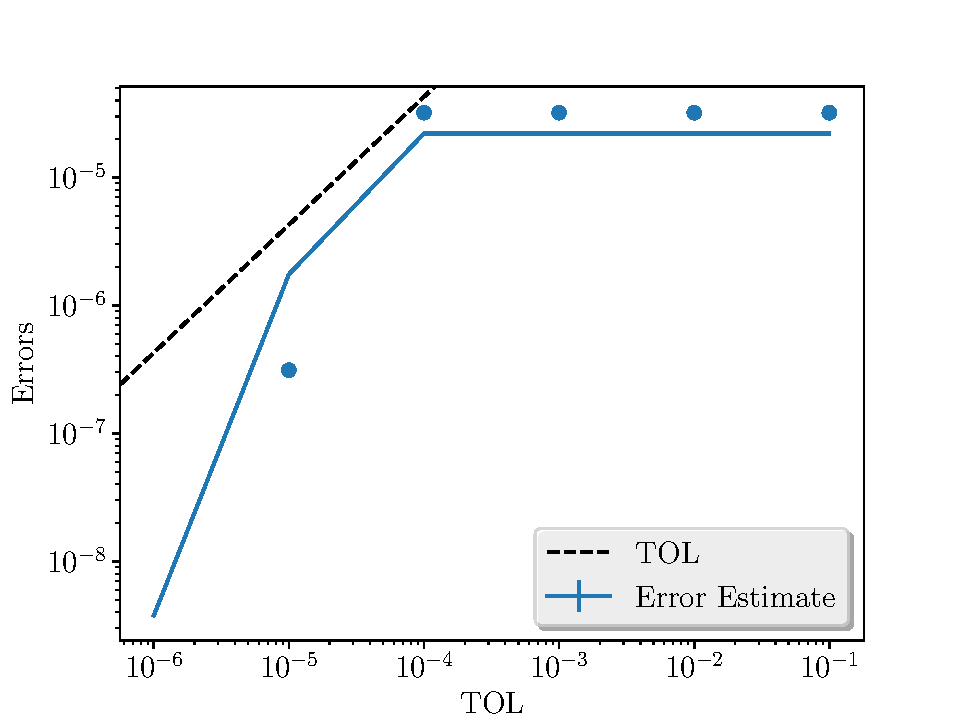
\includegraphics[width=1\linewidth]{./figures/3D_basket/error_estimate.pdf}
		\caption{Error estimate}
		\label{fig:misc_3D_Basket_sub1}
	\end{subfigure}%
	\begin{subfigure}{.4\textwidth}
		\centering
		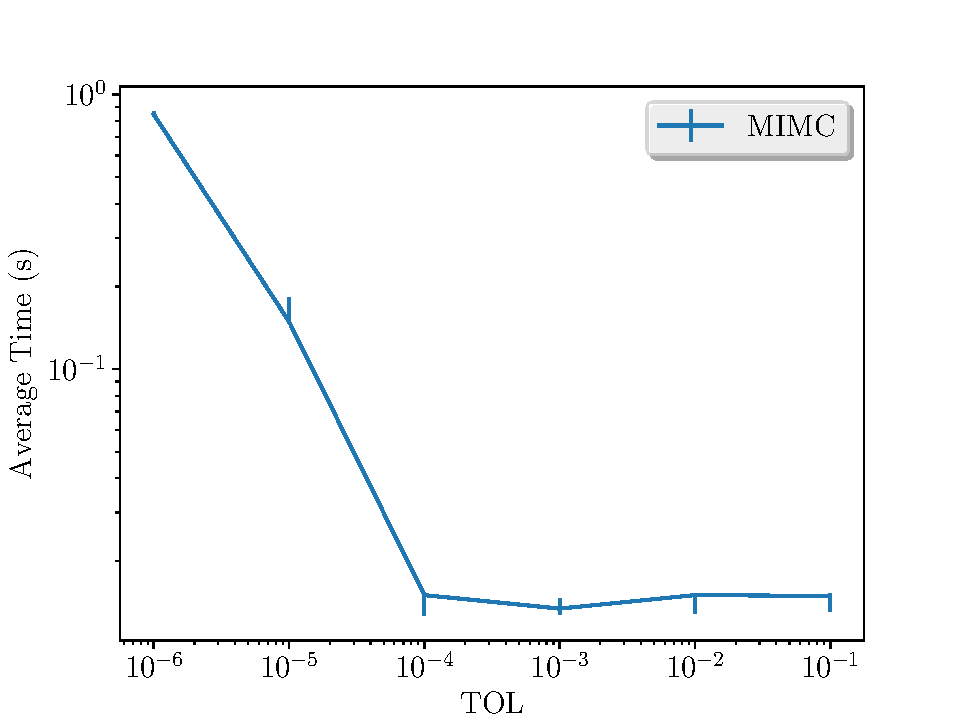
\includegraphics[width=1\linewidth]{./figures/3D_basket/average_running_time.pdf}
		\caption{Average running time as a function of $TOL$}
		\label{fig:misc_3D_Basket_sub2}
	\end{subfigure}%
	\caption{Convergence and complexity results for the $3$-dimensional basket option using BS model.}
	\label{fig:misc_3D_Basket_1}
\end{figure}



\begin{figure}[!h]
	\centering
	\begin{subfigure}{.4\textwidth}
		\centering
		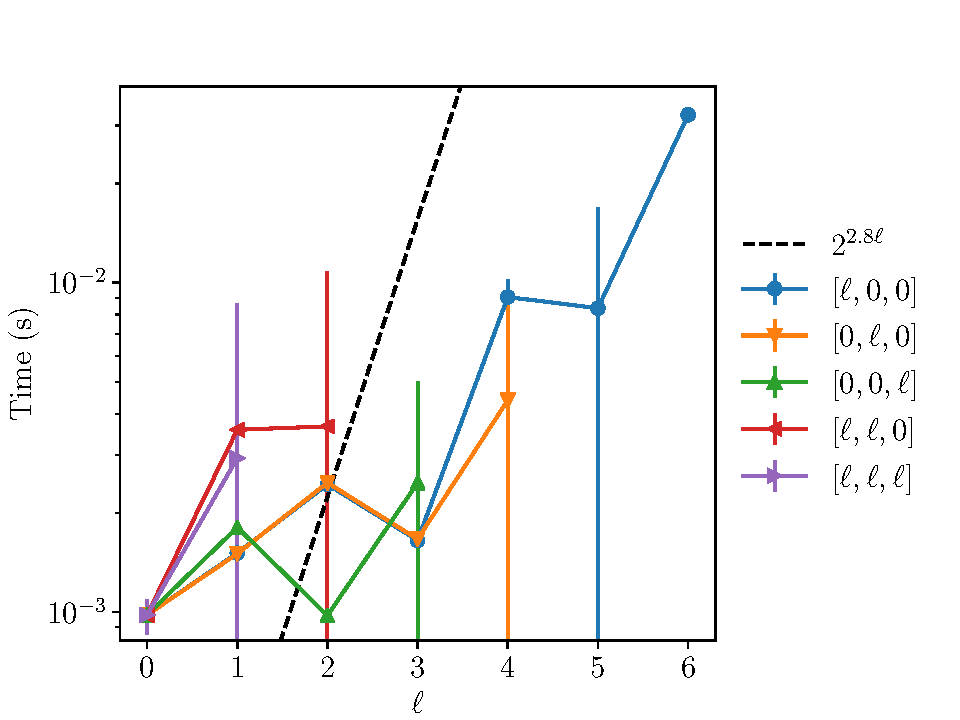
\includegraphics[width=1\linewidth]{./figures/3D_basket/level_work.pdf}
		\caption{Average Computational time per level.}
		\label{fig:misc_3D_Basket_sub3}
	\end{subfigure}%
	\begin{subfigure}{.4\textwidth}
		\centering
		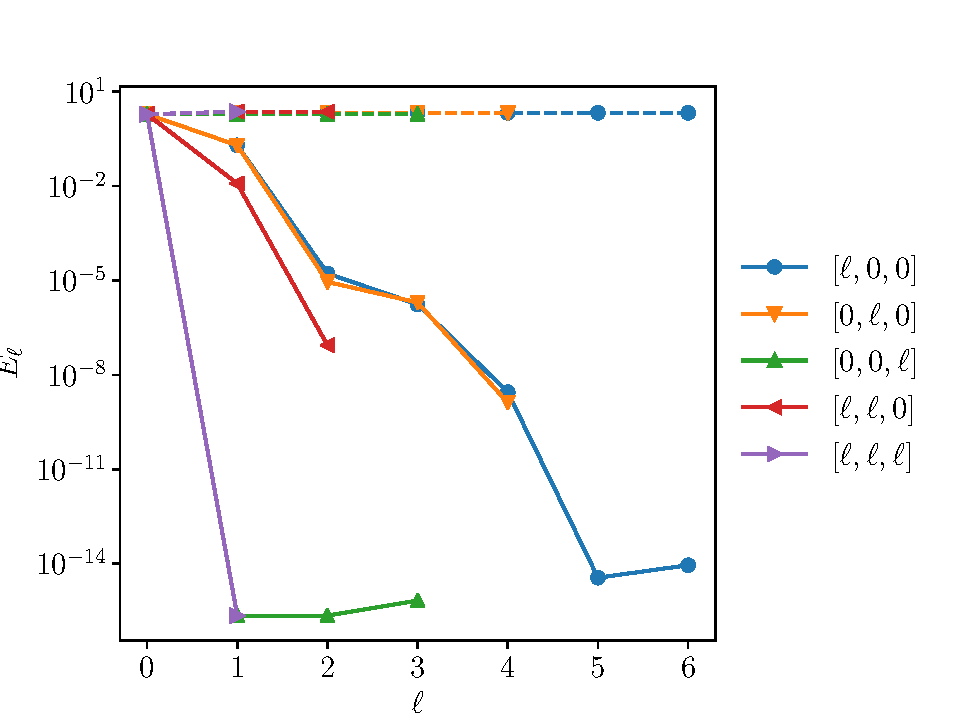
\includegraphics[width=1\linewidth]{./figures/3D_basket/levels_error_rate.pdf}
		\caption{The convergence rate of mixed differences per level.}
		\label{fig:misc_3D_Basket_sub4}
	\end{subfigure}%
	\caption{Convergence and work rates for discretization levels for the $3$-dimensional basket option using BS model.}
	\label{fig:misc_3D_Basket_2}
\end{figure}

\FloatBarrier


\subsubsection{Case of $8$-dimensional Basket}
\begin{figure}[!h]
	\centering
	\begin{subfigure}{.4\textwidth}
		\centering
		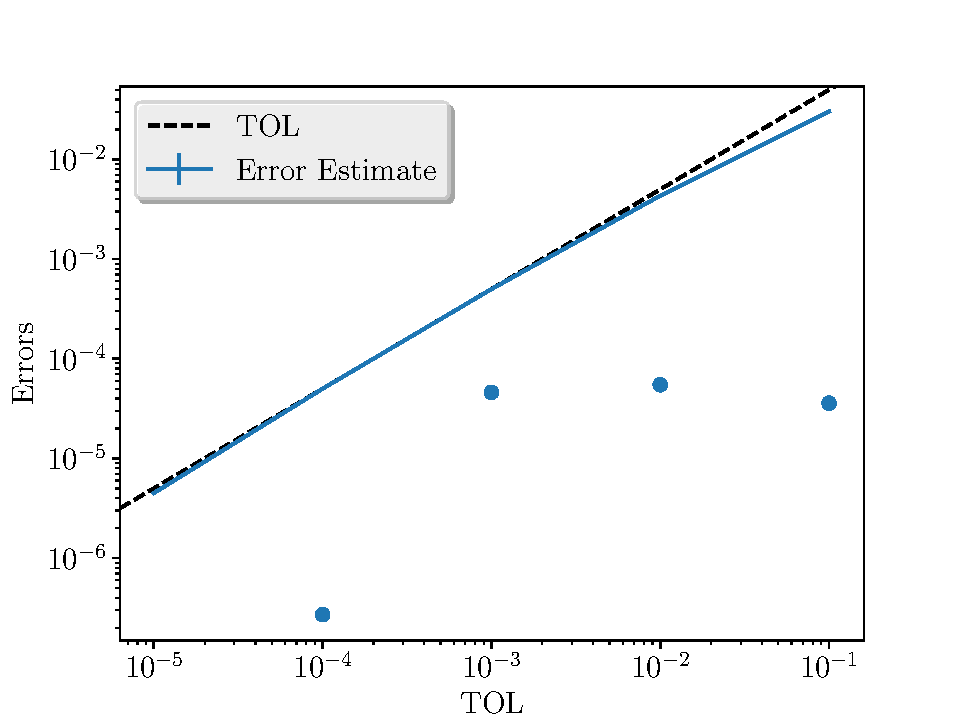
\includegraphics[width=1\linewidth]{./figures/8D_basket/error_estimate.pdf}
		\caption{Error estimate}
		\label{fig:misc_8D_Basket_sub1}
	\end{subfigure}%
	\begin{subfigure}{.4\textwidth}
		\centering
		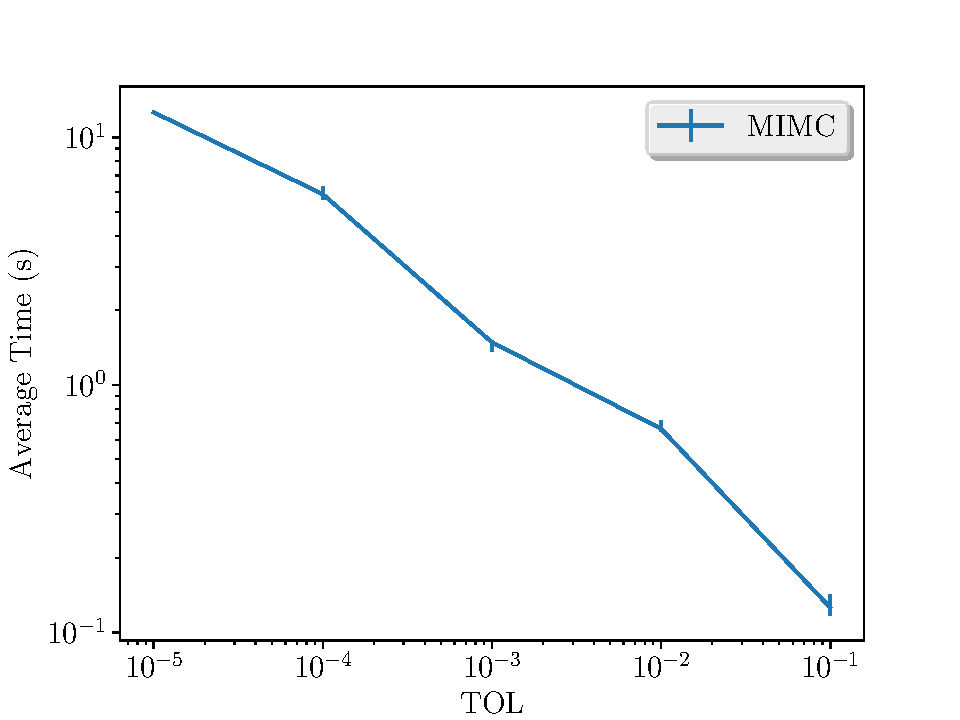
\includegraphics[width=1\linewidth]{./figures/8D_basket/average_running_time.pdf}
		\caption{Average running time as a function of $TOL$}
		\label{fig:misc_8D_Basket_sub2}
	\end{subfigure}%
	\caption{Convergence and complexity results for  the $8$-dimensional basket option using BS model.}
	\label{fig:misc_8D_Basket_1}
\end{figure}



\begin{figure}[!h]
	\centering
	\begin{subfigure}{.4\textwidth}
		\centering
		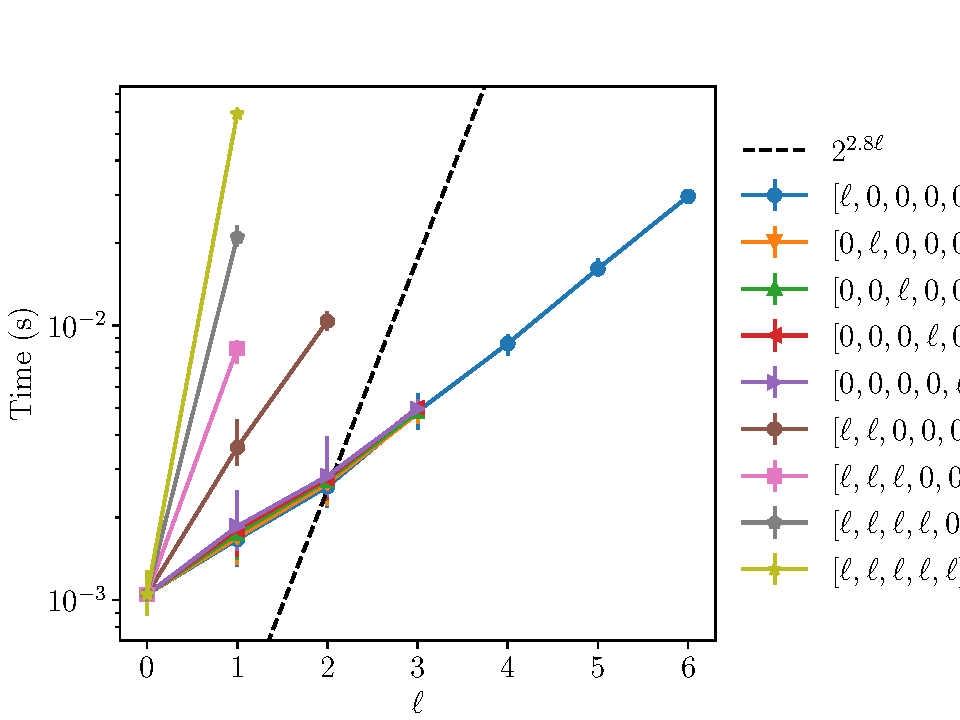
\includegraphics[width=1\linewidth]{./figures/8D_basket/level_work.pdf}
		\caption{Average Computational time per level.}
		\label{fig:misc_8D_Basket_sub3}
	\end{subfigure}%
	\begin{subfigure}{.4\textwidth}
		\centering
		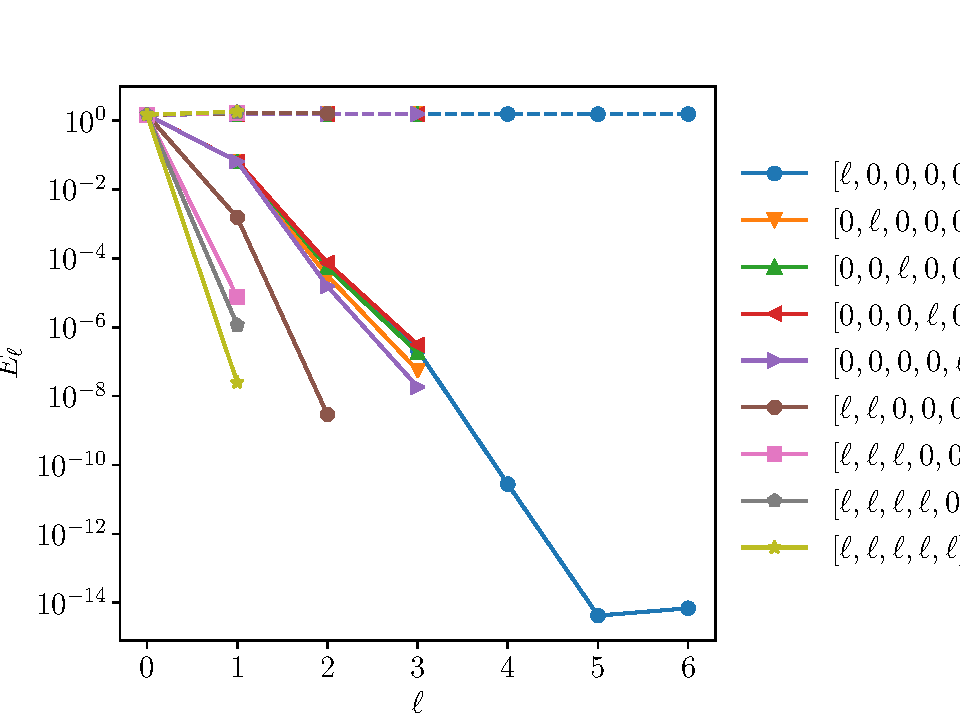
\includegraphics[width=1\linewidth]{./figures/8D_basket/levels_error_rate.pdf}
		\caption{The convergence rate of mixed differences per level.}
		\label{fig:misc_8D_Basket_sub4}
	\end{subfigure}%
	\caption{Convergence and work rates for discretization levels for the $8$-dimensional basket option using BS model.}
	\label{fig:misc_8D_Basket_2}
\end{figure}
\FloatBarrier

\subsubsection{Case of $25$-dimensional Basket}
\begin{figure}[h!]
	\centering
	\begin{subfigure}{.4\textwidth}
		\centering
		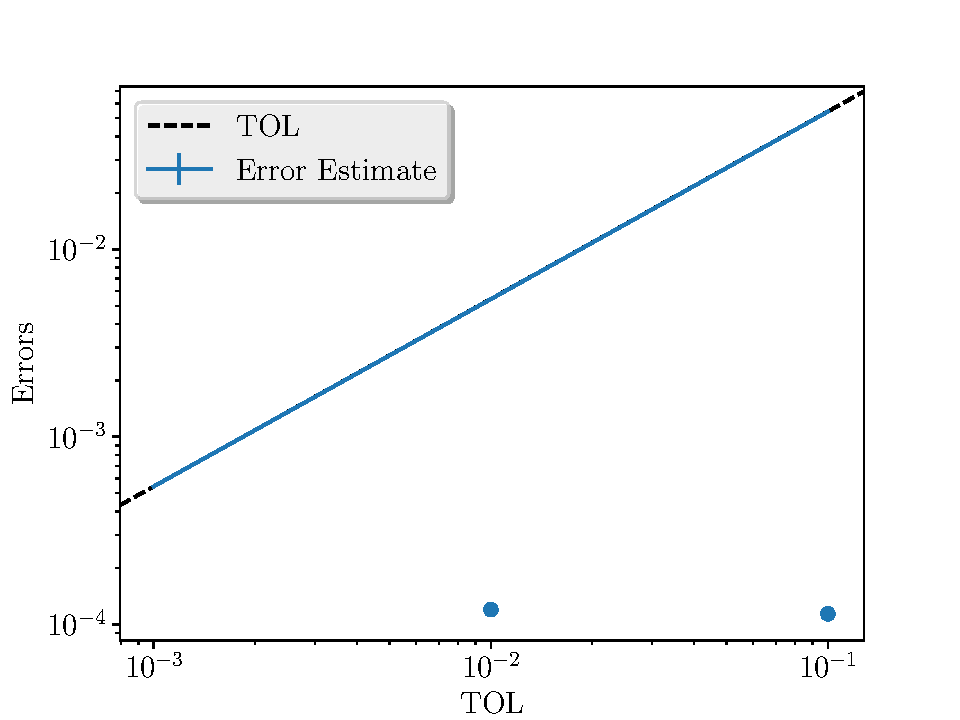
\includegraphics[width=1\linewidth]{./figures/25D_basket/error_estimate.pdf}
		\caption{Error estimate}
		\label{fig:misc_25D_Basket_sub1}
	\end{subfigure}%
	\begin{subfigure}{.4\textwidth}
		\centering
		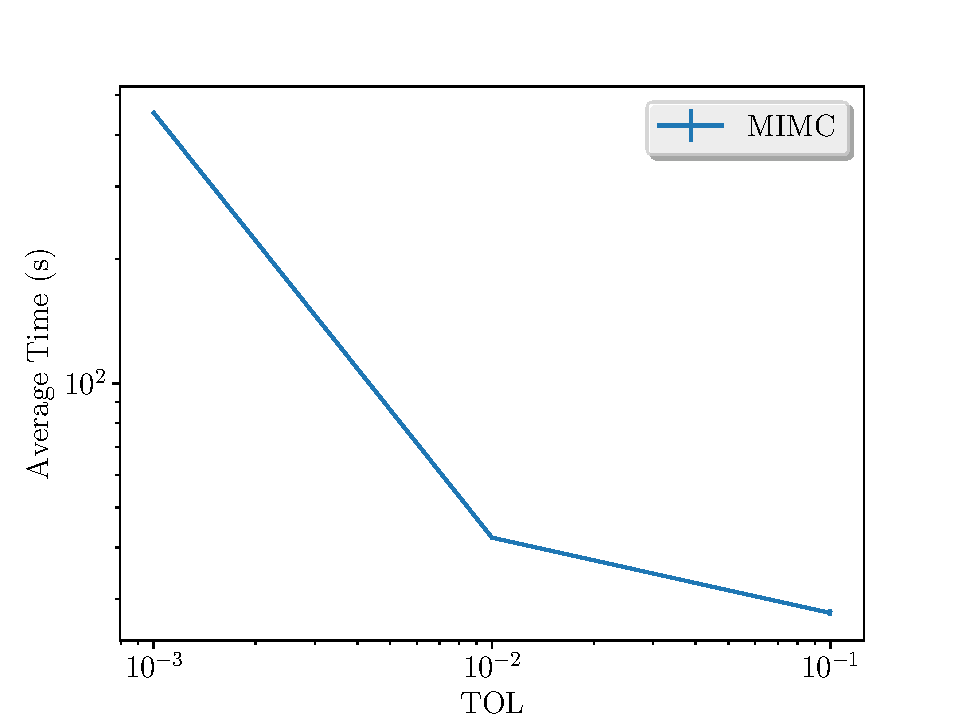
\includegraphics[width=1\linewidth]{./figures/25D_basket/average_running_time.pdf}
		\caption{Average running time as a function of $TOL$}
		\label{fig:misc_25D_Basket_sub2}
	\end{subfigure}%
	\caption{Convergence and complexity results for  the $25$-dimensional basket option using BS model.}
	\label{fig:misc_25D_Basket_1}
\end{figure}



\begin{figure}[h!]
	\centering
	\begin{subfigure}{.4\textwidth}
		\centering
		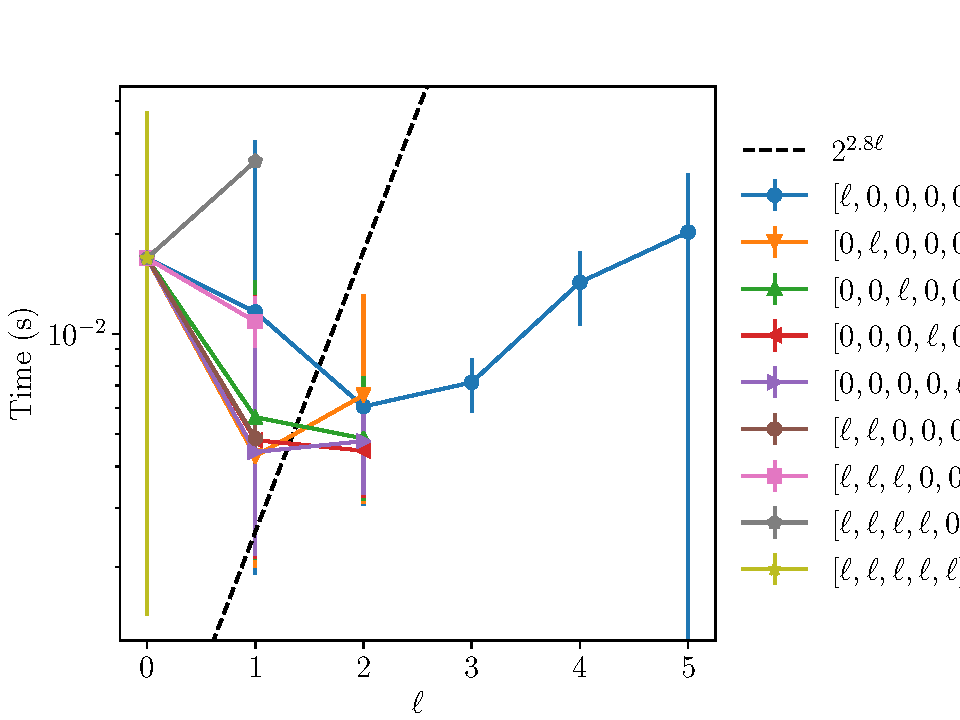
\includegraphics[width=1\linewidth]{./figures/25D_basket/level_work.pdf}
		\caption{Average Computational time per level.}
		\label{fig:misc_25D_Basket_sub3}
	\end{subfigure}%
	\begin{subfigure}{.4\textwidth}
		\centering
		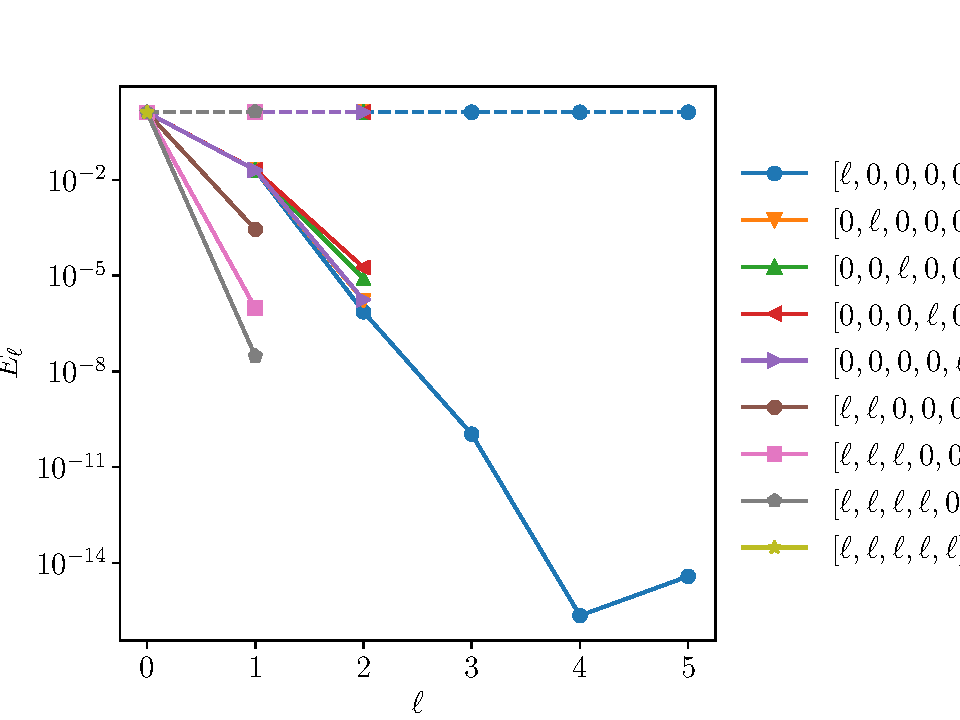
\includegraphics[width=1\linewidth]{./figures/25D_basket/levels_error_rate.pdf}
		\caption{The convergence rate of mixed differences per level.}
		\label{fig:misc_25D_Basket_sub4}
	\end{subfigure}%
	\caption{Convergence and work rates for discretization levels for the $25$-dimensional basket option using BS model.}
	\label{fig:misc_25D_Basket_2}
\end{figure}


\FloatBarrier

%\section{ Prices for different methods for binary option }\label{appendix:Call prices for different methods_binary}
%
%\begin{table}[h!]
%	\centering
%	\begin{tabular}{l*{6}{c}r}
%		Method \textbackslash  Steps            & $2$ & $4$ & $8$ & $16$ &   \\
%		\hline
%		MISC ($TOl=5.10^{-1}$)  & $\red{0.4619}$ & $  \red{0.4404}$ & $\red{0.4299}$ & $\red{0.4250}$  \\
%		\hline
%	\end{tabular}
%	\caption{ Binary option price of the different methods for different number of time steps, without Richardson extrapolation.}
%	\label{table: Binary option price of the different methods for different number of time steps}
%\end{table}
%
%
%\begin{table}[h!]
%	\centering
%	\begin{tabular}{l*{6}{c}r}
%		Method \textbackslash  Steps   &$1-2$         & $2-4$ & $4-8$ & $8-16$  \\
%		\hline
%		MISC ($TOl=5.10^{-1}$) & $\red{0.4239}$ & $0.4188$ & $  0.4194$ & $0.4200$   \\
%			MISC ($TOl=10^{-2}$) & $-$ & $\red{0.4192}$ & $  0.4194$ & $0.4201$   \\
%			MISC ($TOl=10^{-3}$) & $-$ & $-$ & $  \red{0.4198}$ & $\red{0.4205}$   \\
%		\hline
%	\end{tabular}
%	\caption{Binary  option price of the different methods for different number of time steps, with Richardson extrapolation (level $1$).}
%	\label{table: Binary option price of the different methods for different number of time steps, binary option, with richardson, level 1}
%\end{table}
%
%\newpage
%
%
%\section{ Call prices for different methods}\label{appendix:Call prices for different methods}
%
%\begin{table}[h!]
%	\centering
%	\begin{tabular}{l*{6}{c}r}
%		Method \textbackslash  Steps            & $2$ & $4$ & $8$ & $16$ &   \\
%		\hline
%		MISC ($TOl=5.10^{-1}$)  & $\red{16.2145}$ & $16.1352$ & $\red{16.0275}$ & $\red{15.9594}$  \\
%			MISC ($TOl=10^{-3}$)  & $-$ & $ \red{16.1328 }$ & $-$ & $-$  \\
%		\hline
%	\end{tabular}
%	\caption{ Call option price of the different methods for different number of time steps, without Richardson extrapolation.}
%	\label{table: Call option price of the different methods for different number of time steps}
%\end{table}
%
%
%\begin{table}[h!]
%	\centering
%	\begin{tabular}{l*{6}{c}r}
%		Method \textbackslash  Steps   &$1-2$         & $2-4$ & $4-8$ & $8-16$  \\
%		\hline
%		MISC ($TOl=5.10^{-1}$) & $\red{16.4419}$ & $16.0558$ & $15.9205$ & $15.8915$   \\
%		MISC ($TOl=10^{-3}$) & $-$ & $\red{16.0510}$ & $ \red{15.9177}$ & $\red{15.8880}$   \\
%		\hline
%	\end{tabular}
%	\caption{Call  option price of the different methods for different number of time steps, with Richardson extrapolation (level $1$).}
%	\label{table: Call option price of the different methods for different number of time steps, binary option, with richardson, level 1}
%\end{table}
%
%\begin{table}[h!]
%	\centering
%	\begin{tabular}{l*{6}{c}r}
%		Method \textbackslash  Steps   &$1-2-4$         & $2-4-8$ & $4-8-16$   \\
%		\hline
%		MISC ($TOl=5.10^{-1}$) & $15.9269$ & $15.8756$ & $15.8815$  \\
%		MISC ($TOl=10^{-3}$) & $\red{15.9205}$ & $\red{15.8732}$ & $ \red{  15.8789}$   \\
%		\hline
%	\end{tabular}
%	\caption{Call option price of the different methods for different number of time steps, with Richardson extrapolation (level $2$).}
%	\label{table: Call option price of the different methods for different number of time steps, binary option, with richardson, level 2}
%\end{table}
%\newpage



%
%\section{Results of the basket example}
%\subsubsection{Verifying bounds on work and error contributions}
%
%In this subsection, we discuss the validity of Assumptions $2$-$4$ in \cite{haji2016multi}, upon which the MISC convergence theorem is based. In this case, basket option case we do not use a deterministic solver since the we have a close for of the integrand and then  we analyze  only the properties of the collocation method applied to
%the problem.
%
%
%
%
%Below, we show in figures (\ref{fig:test_basket_1},\ref{fig:test_basket_2},\ref{fig:test_basket_3}) the rate of convergence of first and mixed differences for different orders and we check that the error is decaying exponentially wrt number of points used in the quadrature.
%
%	
%	\begin{figure}[h!]
%		\centering
%		\begin{subfigure}{.5\textwidth}
%			\centering
%			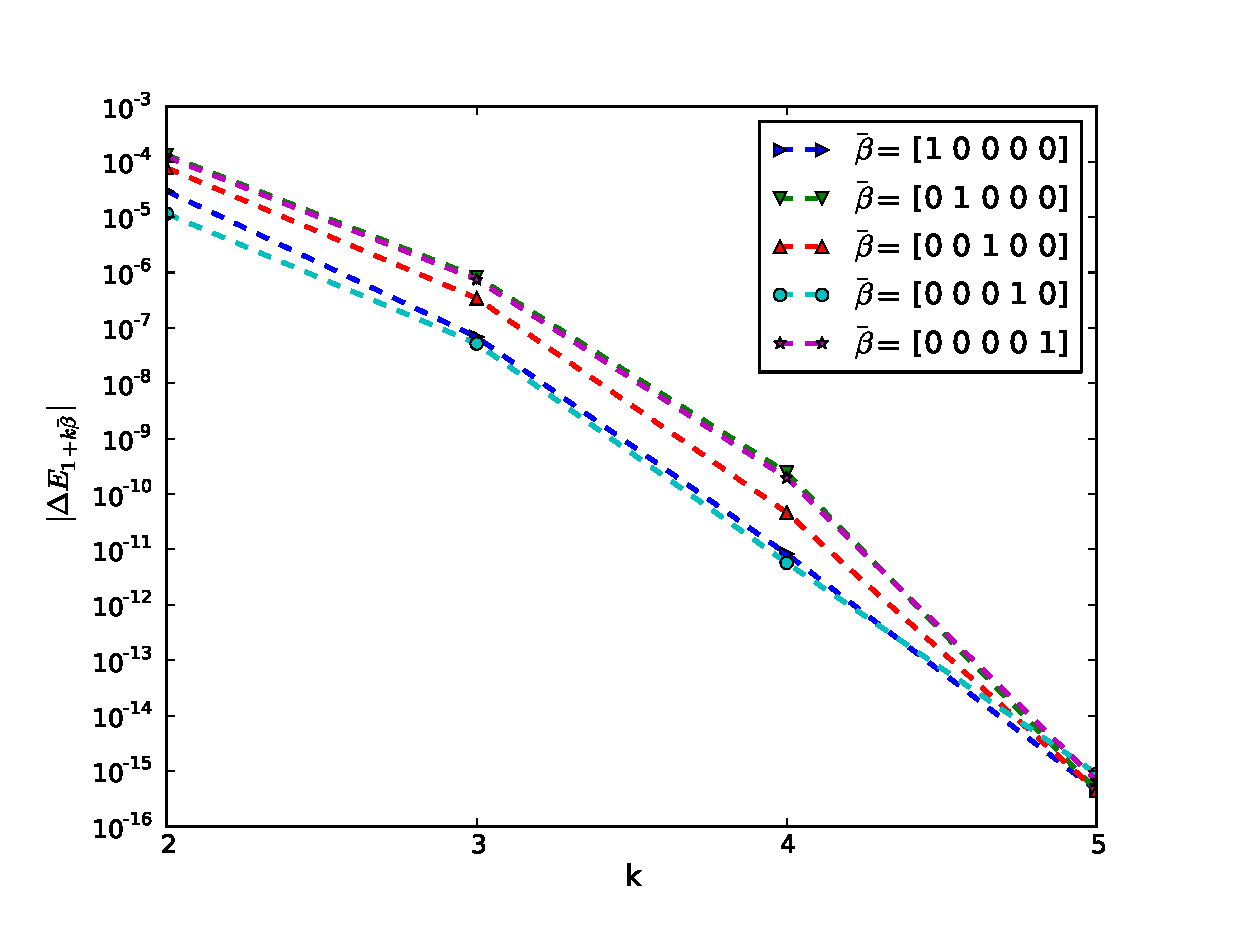
\includegraphics[width=1\linewidth]{./figures/first_difference_basket.eps}
%			\caption{}
%			\label{fig:sub1}
%		\end{subfigure}%
%		\begin{subfigure}{.5\textwidth}
%			\centering
%			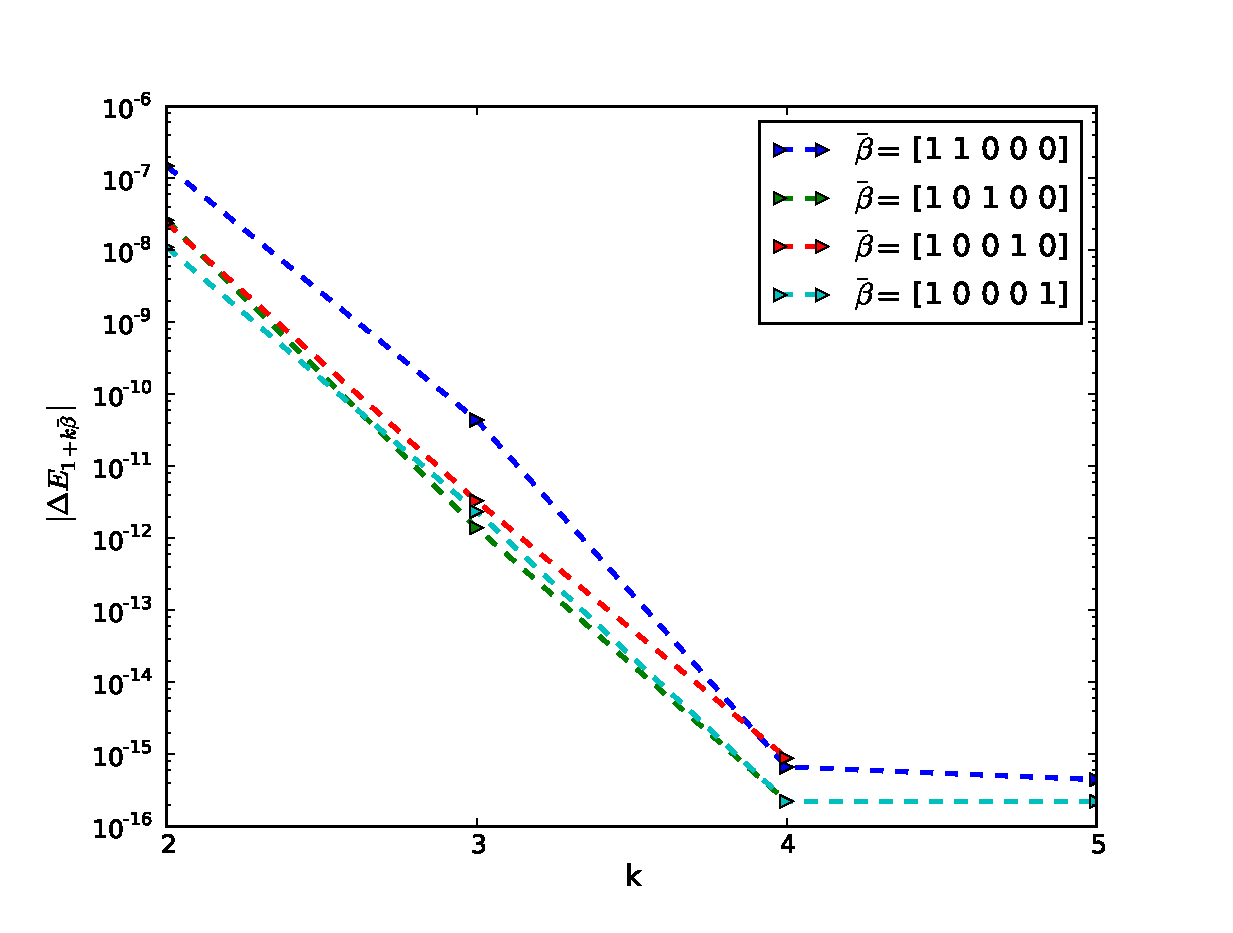
\includegraphics[width=1\linewidth]{./figures/mixed_difference_order2_basket_1.eps}
%			\caption{}
%			\label{fig:sub2}
%		\end{subfigure}%
%		\caption{The rate of convergence of $\abs{\Delta E_{\beta}}$ ($\beta=\mathbf{1}+k \bar{\beta}$): a) shows the rate of convergence of first order differences. b)  shows the rate of convergence of second order mixed differences.}
%			\label{fig:test_basket_1}
%	\end{figure}
%
%	\begin{figure}
%	\centering
%	\begin{subfigure}{.5\textwidth}
%		\centering
%		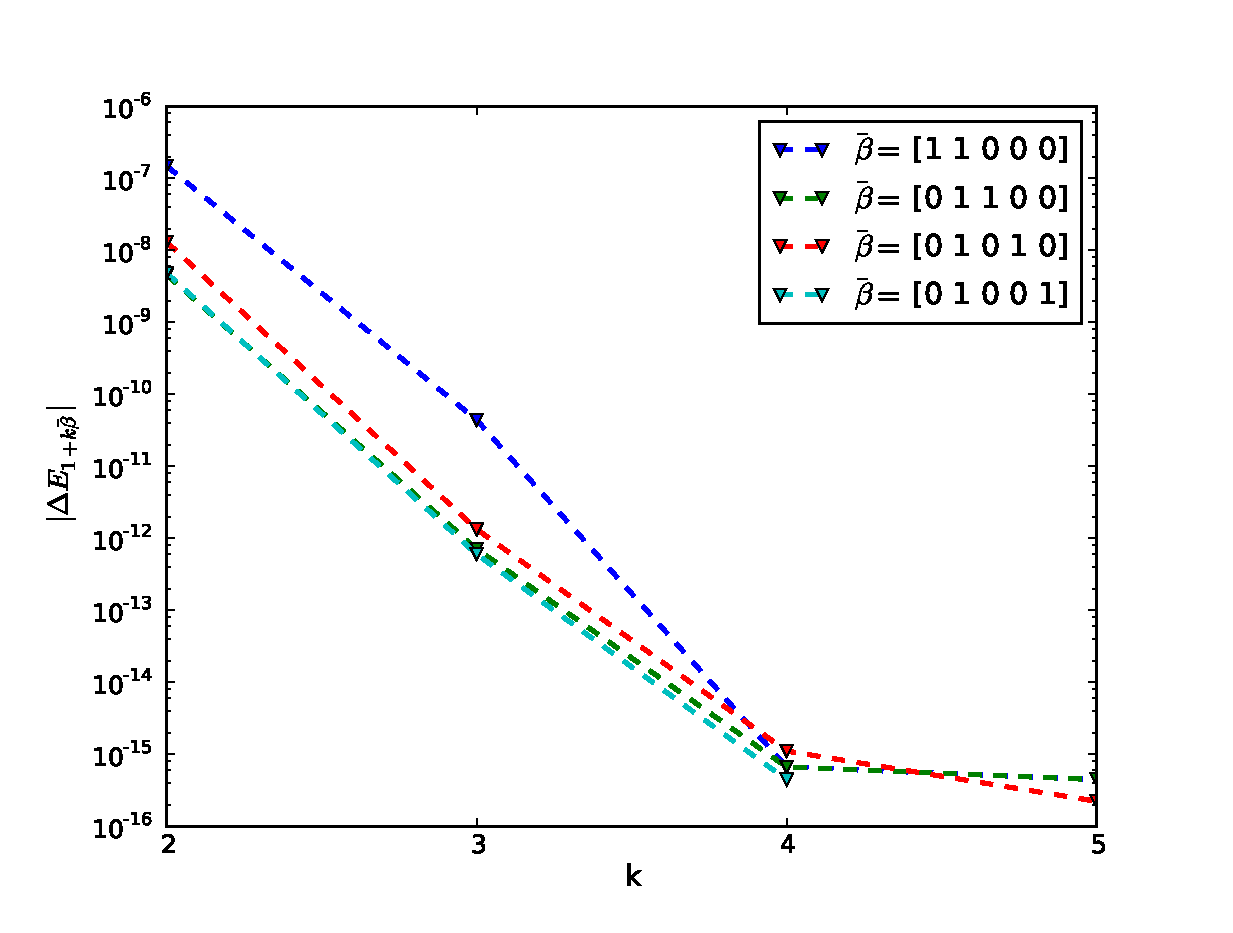
\includegraphics[width=1\linewidth]{./figures/mixed_difference_order2_basket_2.eps}
%		\caption{}
%		\label{fig:sub3}
%	\end{subfigure}%
%	\begin{subfigure}{.5\textwidth}
%		\centering
%		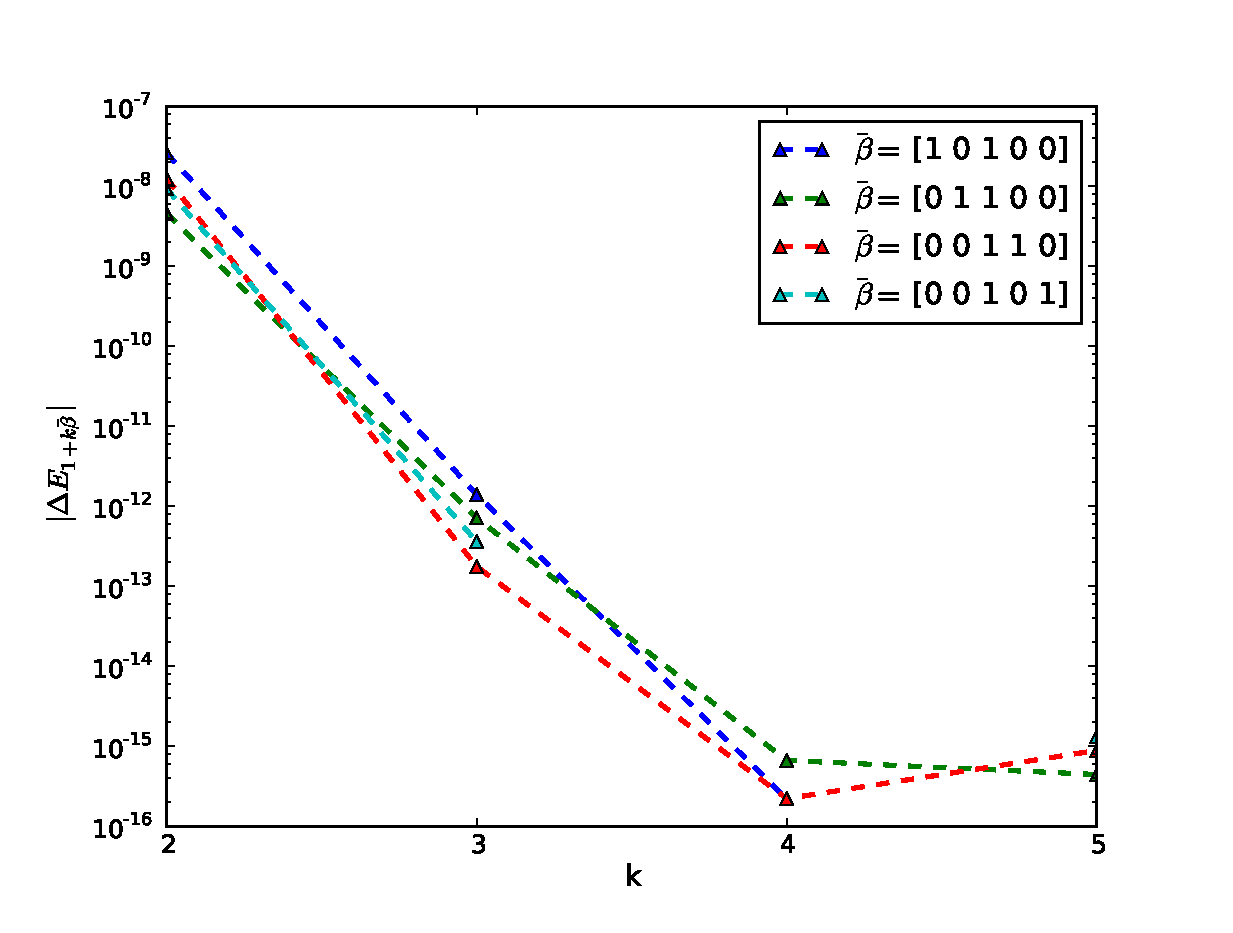
\includegraphics[width=1\linewidth]{./figures/mixed_difference_order2_basket_3.eps}
%		\caption{}
%		\label{fig:sub4}
%	\end{subfigure}
%
%	\caption{The rate of convergence of $\abs{\Delta E_{\beta}}$ ($\beta=\mathbf{1}+k \bar{\beta}$)): a) and b) show  the rate of convergence of second order mixed differences for different settings.}
%		\label{fig:test_basket_2}
%\end{figure}
%
%	\begin{figure}
%	\centering
%	\begin{subfigure}{.5\textwidth}
%		\centering
%		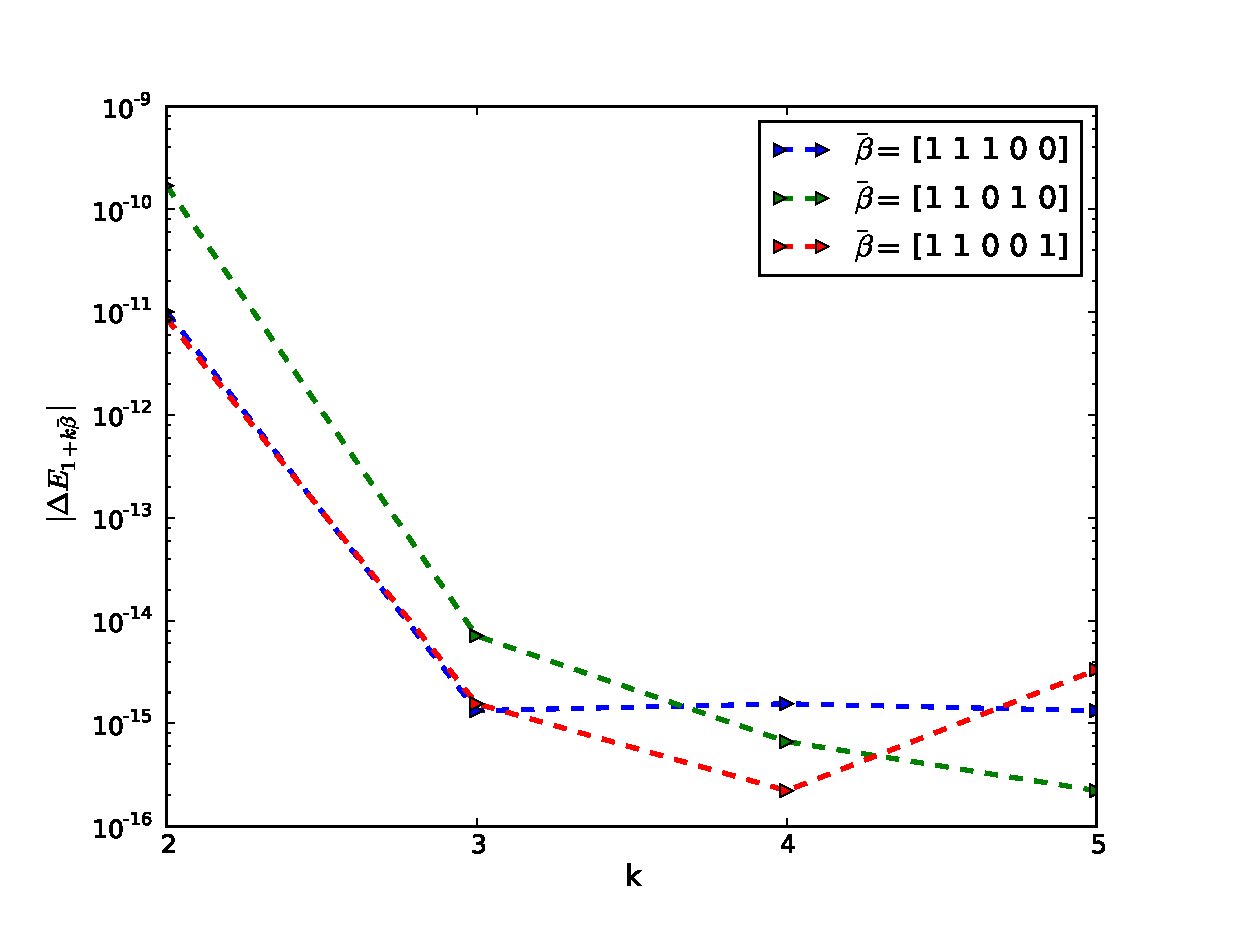
\includegraphics[width=1\linewidth]{./figures/mixed_difference_order3_basket_1.eps}
%	    \caption{}
%		\label{fig:sub5}
%	\end{subfigure}%
%	\begin{subfigure}{.5\textwidth}
%		\centering
%		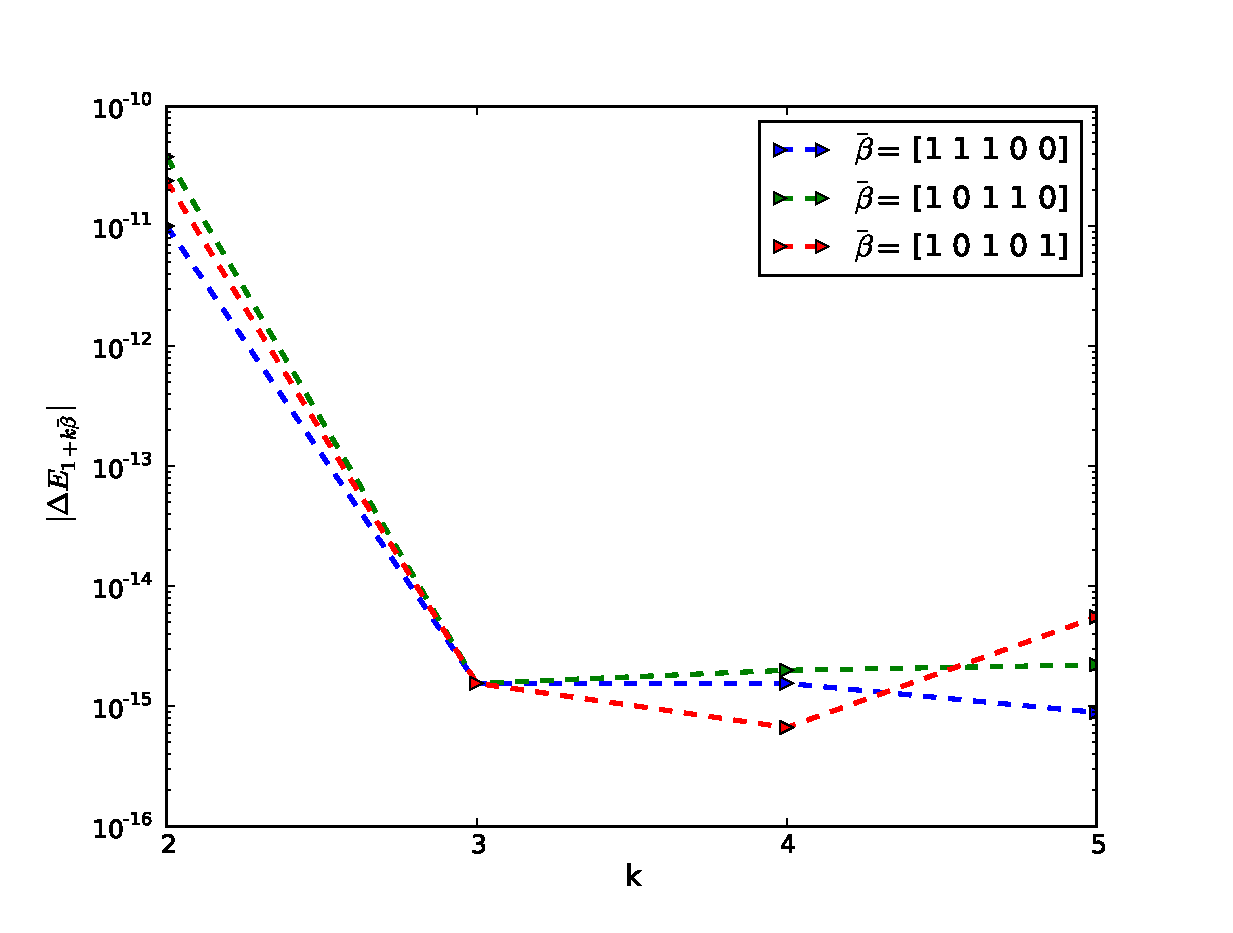
\includegraphics[width=1\linewidth]{./figures/mixed_difference_order3_basket_2.eps}
%		\caption{}
%		\label{fig:sub6}
%	\end{subfigure}
%	
%	\caption{The rate of convergence of $\abs{\Delta E_{\beta}}$ ($\beta=\mathbf{1}+k \bar{\beta}$): a) and b) show  the rate of convergence of third order mixed differences for different settings.}
%	\label{fig:test_basket_3}
%\end{figure}
%
%
%
% \newpage
%\section{Implementation details and  MISC results}\label{sec:Implementation details and  MISC results}
%The first step, when testing this example is to fix $\Delta t_{\text{min}}$ for the  time discretization parameter and do not introduce a hierarchy of levels in the deterministic dimension. Therefore, we will only construct a hierarchy of levels in the stochastic dimension associated with the Brownian increments. Then, the second step is to avoid this restriction of minimum  time discretization parameter (somehow like letting $\Delta t_{\text{min}} \rightarrow 0$)  and in that case, the problem will be close to do the integration in $\infty$-dimension, we need to see how the convergence rates will behave. The third step, is to use Richardson extrapolation which we expect bring the order of convergence for the Euler scheme from $ \ordo{\Delta t}$  to  $\ordo{\Delta t^2}$, and then we may expect that we will need fewer time steps to converge than the first case, and which means that fewer stochastic directions will be activated.   One technical difference here is that for $1$-dimensional, we will have two kink points instead of one but the procedure will be the same.  We note that we used Laguerre quadrature for integrating with respect to the dimension containing the kink. 
%
%Since we observed some problems for the results of the non-smooth payoff with Richardson extrapolation, we tried to add another case where we use a smoothed version of the call payoff to figure out the source of the problem. Using a smooth payoff allow us to separate the effect of infinite dimension and non-smoothness. As a possible choice, we use  the Black Scholes call option price formula, given by 
%\begin{equation}
%\mathrm C(\mathrm S,\mathrm t)= \mathrm N(\mathrm d_1)\mathrm S - \mathrm N(\mathrm d_2) \mathrm K \mathrm e^{-rt}
%\label{eq:2}
%\end{equation}
%
%\begin{equation}
%\mathrm d_1= \frac{1}{\sigma \sqrt{\mathrm t}} \left[\ln{\left(\frac{S}{K}\right)} + t\left(r + \frac{\sigma^2}{2} \right) \right]
%\end{equation}
%
%\begin{equation}
%\mathrm d_2= d_1- \sigma  \sqrt{t} 
%\end{equation}
%
%\begin{equation}
%N(x)=\frac{1}{\sqrt{2\pi}} \int_{-\infty}^{x} \mathrm e^{-\frac{1}{2}z^2} dz
%\label{eq:5}
%\end{equation}
%
%
%, which can be seen as a smoothed version of the true payoff (See figure \ref{fig:smooth_non_smooth}). The two differences with respect to the non-smooth case is that the dimension of the parameter space (stochastic space) now is increased by one  due to including the terminal value of the driving Brownian motion. Numerically, we observed weird results , in fact the quadrature performed worse than with the non-smooth case,  even for various values of volatilities. We still need to understand why this choice is not a good one. 
%
%
%Another possible choice that we worked with,  is by using the following smooth approximation of the max call payoff (See figure \ref{fig:smooth_payoff2})
%
%\begin{align}\label{eq:smooth_payoff2}
%	\operatorname{\max}_\epsilon(S-K,0) \approx 0.5 ( S-K+\sqrt{ (S-K)^{2}+\epsilon}),
%\end{align}
%
%where $\epsilon>0$.
%
%
%
%
%
%
%
%\begin{figure}[!h]
%	\centering
%	\begin{subfigure}{.5\textwidth}
%		\centering
%		\includegraphics[width=1\linewidth]{./figures/smooth_non_smooth_payoff.png}
%		\caption{Black Scholes call option price for different values of $\sigma$}
%		\label{fig:smooth_non_smooth}
%	\end{subfigure}%
%	\begin{subfigure}{.5\textwidth}
%		\centering
%		\includegraphics[width=1\linewidth]{./figures/smooth_payoff_2.png}
%		\caption{Smooth approximation of the max call payoff for different values of $\epsilon$.}
%		\label{fig:smooth_payoff2}
%	\end{subfigure}%
%\end{figure}
%
%
%
%%Numerically, we tried different values of $\epsilon$. For values of $\epsilon<10^5$, it is much expensive to run the quadrature compared to the non-smooth case( we need to understand why we have this behavior). 
%%In section \ref{sec:Results using MISC code_1D_BS}, we show some of the results with $8$ time steps and for $\epsilon=10^5$.
%%
%%\newpage
%%\subsubsection{A smooth payoff with Richardson extrapolation}
%%In this section, we present Richardson extrapolation algorithm that we use to compute the integrand before passing it to misc for the quadrature. We expect a slighter improvement of the rates  compared to cases without using Richardson extrapolation since $dt$ is fixed in the misc code (we assume that we do not have a deterministic direction, just stochastic ones). However, this improvement should be much better as $dt\rightarrow 0$ (higher number of time steps). In fact, since the convergence is fast with respect to the stochastic dimensions, the rate of convergence is deteriorated by the time-stepping procedure and then the advantage of using   Richardson extrapolation is to bring the order of convergence for the Euler scheme from $ \ordo{\Delta t}$  to  $\ordo{\Delta t^\alpha}$ ($\alpha>1$). This improvement implies that fewer stochastic directions will be activated and thus the improvement of the global rate of convergence.
%%
%%\begin{algorithm}
%%	\caption{Description of the Richardson algorithm }\label{euclid}
%%	\begin{algorithmic}[1]
%%%		\Procedure{MyProcedure}{}
%%		\State Initial set of quadrature points $y$, initial number of time steps $N$, $n:$ level of Richardson extrapolation, $\tilde{g}:$ the smooth payoff approximation
%%		\For{\texttt{$i=0$ to $n$}}
%%		\State $d_i0 \leftarrow \tilde{g}(\bar{X}_{N})$  ($\bar{X}_{N}$ is the stock price simulated with $N$ time steps and using $N$ quadrature points form $y$)
%%			\For{\texttt{$j=1$ to $i$}}
%%			\State $d_{i,j} \leftarrow d_{i,j-1}+(d_{i,j-1}-d_{i-1,j-1})/(4^j-1)$
%%			\EndFor
%%		\State $N \leftarrow 2 N	$
%%		\EndFor
%%		
%%		
%%		
%%%		\State $i \gets \textit{patlen}$
%%%		\BState \emph{top}:
%%%		\If {$i > \textit{stringlen}$} \Return false
%%%		\EndIf
%%%		\State $j \gets \textit{patlen}$
%%%		\BState \emph{loop}:
%%%		\If {$\textit{string}(i) = \textit{path}(j)$}
%%%		\State $j \gets j-1$.
%%%		\State $i \gets i-1$.
%%%		\State \textbf{goto} \emph{loop}.
%%%		\State \textbf{close};
%%%		\EndIf
%%%		\State $i \gets i+\max(\textit{delta}_1(\textit{string}(i)),\textit{delta}_2(j))$.
%%%		\State \textbf{goto} \emph{top}.
%%%		\EndProcedure
%%	\end{algorithmic}
%%\end{algorithm}
%%
%%
%%
%%
%
%
%%In the simulation, we  use consistent Brownian increments in simulating the paths of $\hat{X}^h$ and $\hat{X}^{2h}$, which results in a substantial reduction in variance. More specifically, each Brownian increment driving $\hat{X}^{2h}$ is the sum of two of the increments driving $\hat{X}^{h}$. This means that if we use $\sqrt{h} Z_1,\sqrt{h} Z_2,\dots $ as the Brownian increments for  $\hat{X}^{h}$ then we can use  $\sqrt{h} (Z_1+Z_2),\sqrt{h} (Z_3+Z_4),\dots $  as the Brownian increments for $\hat{X}^{2h}$.
%
%
%
%
%
%
%
%
%In table \ref{table: Complexity rates of the different methods for different number of time steps}, we summarize the results that we get in terms of complexity rates for different methods using different number of time steps. We clarify that the results for the Richardson extrapolation are given for just one level, where the associated steps in the table corresponds to those of level $1$.
%\begin{table}[h!]
%	\centering
%	\begin{tabular}{l*{6}{c}r}
%		Method \textbackslash  Steps            & $2$ & $4$ & $8$ & $16$  \\
%		\hline
%		Non-smooth payoff   & $-1/5$ & $-1/5$ & $-2/5$ & $-7/10$  \\
%		Non-smooth payoff with Richardson  extrapolation    & $-$ & $-$ & $-$ & $-$  \\
%		Smooth payoff(given by \eqref{eq:smooth_payoff2},$\epsilon=10^{-5}$)          & $-1/3$ &$-1/3$ &  $-3/5$ &  $-1$ \\
%		Smooth payoff with Richardson  extrapolation      & - & $-1/10$  & $-4/10$ & $-$  \\
%		\hline
%	\end{tabular}
%	\caption{Complexity rates of the different methods for different number of time steps}
%	\label{table: Complexity rates of the different methods for different number of time steps}
%\end{table}	
%
%Detailed plots for each case are given in appendix \ref{app: MISC Results 1D_BS}. Mainly, from the plots, 
%we checked  that we achive the prescribed tolerance using MISC, the convergence rates of mixed differences which is a basic assumption for using MISC (we observe exponential decay of error rates wrt to the number of quadrature points) and finally the complexity rates.
%
%\section{ MISC Results for the call option under discretized BS model}\label{app: MISC Results 1D_BS}
%
%\subsection{Case of $2$ time steps with non-smooth payoff}
%
%From the following plots, we confirm the exponential rate of convergence for the stochastic parameters, we achieve the prescribed tolerance and  we get a rate of complexity (in terms of average running time) approximately of order $-1/5$ for $2$ time steps.
%\begin{figure}[!h]
%	\centering
%	\begin{subfigure}{.5\textwidth}
%		\centering
%		\includegraphics[width=1\linewidth]{./figures/1D_BS_2_steps_non_smooth/error_estimate.pdf}
%		\caption{Error estimate}
%		\label{fig:misc_1D_BS_non_smooth_2steps_sub1}
%	\end{subfigure}%
%	\begin{subfigure}{.5\textwidth}
%		\centering
%		\includegraphics[width=1\linewidth]{./figures/1D_BS_2_steps_non_smooth/average_running_time.pdf}
%		\caption{Average running time as a function of $TOL$}
%		\label{fig:misc_1D_BS_non_smooth_2steps_sub2}
%	\end{subfigure}%
%	\caption{Convergence and complexity results for for the $1D$ BS model with the non-smooth call payoff.}
%	\label{fig:misc_1D_BS_nonsmooth_2steps_2}
%\end{figure}
%
%
%
%\begin{figure}[!h]
%	\centering
%	\begin{subfigure}{.5\textwidth}
%		\centering
%		\includegraphics[width=0.95\linewidth]{./figures/1D_BS_2_steps_non_smooth/level_work.pdf}
%		\caption{Average Computational time per level}
%		\label{fig:misc_1D_BS_non_smooth_2steps_sub3}
%	\end{subfigure}%
%	\begin{subfigure}{.5\textwidth}
%		\centering
%		\includegraphics[width=0.95\linewidth]{./figures/1D_BS_2_steps_non_smooth/levels_error_rate.pdf}
%		\caption{ The convergence rate of first differences per level}
%		\label{fig:misc_1D_BS_non_smooth_2steps_sub4}
%	\end{subfigure}%
%	\caption{Convergence and work rates for discretization levels for the $1D$ BS model with the non-smooth call payoff.}
%	\label{fig:misc_1D_BS_2teps_2}
%\end{figure}
%
%
%
%\subsection{Case of $2$ time steps with smooth payoff (given by \eqref{eq:smooth_payoff2})}
%
%From the following plots, we confirm the exponential rate of convergence for the stochastic parameters, we achieve the prescribed tolerance and  we get a rate of complexity (in terms of average running time) approximately of order $-1/3$ for $2$ time steps.
%
%\begin{figure}[!h]
%	\centering
%	\begin{subfigure}{.5\textwidth}
%		\centering
%		\includegraphics[width=1\linewidth]{./figures/1D_BS_2_steps_smooth_second_payoff_eps_10_5/error_estimate.pdf}
%		\caption{Error estimate}
%		\label{fig:misc_1D_BS_2_steps_smooth_second_payoff_eps_10_5_sub1}
%	\end{subfigure}%
%	\begin{subfigure}{.5\textwidth}
%		\centering
%		\includegraphics[width=1\linewidth]{./figures/1D_BS_2_steps_smooth_second_payoff_eps_10_5/average_running_time.pdf}
%		\caption{Average running time as a function of $TOL$}
%		\label{fig:misc_1D_BS_2_steps_smooth_second_payoff_eps_10_5_sub2}
%	\end{subfigure}%
%	\caption{Convergence and complexity results for for the $1D$ BS model with the smooth call payoff given by \eqref{eq:smooth_payoff2}.}
%	\label{fig:misc_1D_BS_2_steps_smooth_second_payoff_eps_10_5_1}
%\end{figure}
%
%
%
%\begin{figure}[!h]
%	\centering
%	\begin{subfigure}{.5\textwidth}
%		\centering
%		\includegraphics[width=0.95\linewidth]{./figures/1D_BS_2_steps_smooth_second_payoff_eps_10_5/level_work.pdf}
%		\caption{Average Computational time per level}
%		\label{fig:misc_1D_BS_2_steps_smooth_second_payoff_eps_10_5_sub3}
%	\end{subfigure}%
%	\begin{subfigure}{.5\textwidth}
%		\centering
%		\includegraphics[width=0.95\linewidth]{./figures/1D_BS_2_steps_smooth_second_payoff_eps_10_5/levels_error_rate.pdf}
%		\caption{ The convergence rate of first differences per level}
%		\label{fig:misc_1D_BS_2_steps_smooth_second_payoff_eps_10_5_sub4}
%	\end{subfigure}%
%	\caption{Convergence and work rates for discretization levels for the $1D$ BS model with the smooth call payoff given by \eqref{eq:smooth_payoff2}.}
%	\label{fig:misc_1D_BS_2_steps_smooth_second_payoff_eps_10_5_2}
%\end{figure}
%
%
%\newpage
%
%
%
%
%\subsection{Case of $4$ time steps with non-smooth payoff}
%
%From the following plots, we confirm the exponential rate of convergence for the stochastic parameters, we achieve the prescribed tolerance and  we get a rate of complexity (in terms of average running time) approximately of order $-1/5$ for $4$ time steps.
%\begin{figure}[!h]
%	\centering
%	\begin{subfigure}{.5\textwidth}
%		\centering
%		\includegraphics[width=1\linewidth]{./figures/1D_BS_4_steps_non_smooth/error_estimate.pdf}
%		\caption{Error estimate}
%		\label{fig:misc_1D_BS_non_smooth_4steps_sub1}
%	\end{subfigure}%
%	\begin{subfigure}{.5\textwidth}
%		\centering
%		\includegraphics[width=1\linewidth]{./figures/1D_BS_4_steps_non_smooth/average_running_time.pdf}
%		\caption{Average running time as a function of $TOL$}
%		\label{fig:misc_1D_BS_non_smooth_4steps_sub2}
%	\end{subfigure}%
%	\caption{Convergence and complexity results for for the $1D$ BS model with the non-smooth call payoff .}
%	\label{fig:misc_1D_BS_nonsmooth_4steps_2}
%\end{figure}
%
%
%
%\begin{figure}[!h]
%	\centering
%	\begin{subfigure}{.5\textwidth}
%		\centering
%		\includegraphics[width=0.95\linewidth]{./figures/1D_BS_4_steps_non_smooth/level_work.pdf}
%		\caption{Average Computational time per level}
%		\label{fig:misc_1D_BS_non_smooth_4steps_sub3}
%	\end{subfigure}%
%	\begin{subfigure}{.5\textwidth}
%		\centering
%		\includegraphics[width=0.95\linewidth]{./figures/1D_BS_4_steps_non_smooth/levels_error_rate.pdf}
%		\caption{ The convergence rate of first differences per level}
%		\label{fig:misc_1D_BS_non_smooth_4steps_sub4}
%	\end{subfigure}%
%	\caption{Convergence and work rates for discretization levels for the $1D$ BS model with the non- smooth call payoff.}
%	\label{fig:misc_1D_BS_4teps_2}
%\end{figure}
%
%
%\newpage
%
%\subsection{Case of non smooth payoff  with Richardson extrapolation (level $0$: $2$ time steps, level $1$: $4$ time steps) (Ignoring the middle part of integration)}
%
%From the following plots, we confirm the exponential rate of convergence for the stochastic parameters, we achieve the prescribed tolerance and  we get a rate of complexity (in terms of average running time) approximately of order $-1/2$.
%
%\begin{figure}[!h]
%	\centering
%	\begin{subfigure}{.5\textwidth}
%		\centering
%		\includegraphics[width=1\linewidth]{./figures/1D_BS_2_4_step_non_smooth_richardson_without_middle/error_estimate.pdf}
%		\caption{Error estimate}
%		\label{fig:misc_1D_BS_2_4_step_non_smooth_richardson_without_middle_sub1}
%	\end{subfigure}%
%	\begin{subfigure}{.5\textwidth}
%		\centering
%		\includegraphics[width=1\linewidth]{./figures/1D_BS_2_4_step_non_smooth_richardson_without_middle/average_running_time.pdf}
%		\caption{Average running time as a function of $TOL$}
%		\label{fig:misc_1D_BS_2_4_step_non_smooth_richardson_without_middle_sub2}
%	\end{subfigure}%
%	\caption{Convergence and complexity results for for the $1D$ BS model with the non smooth call payoff with Richardson extrapolation (Ignoring the middle part of integration).}
%	\label{fig:misc_1D_BS_2_4_step_non_smooth_richardson_without_middle_1}
%\end{figure}
%
%
%
%\begin{figure}[!h]
%	\centering
%	\begin{subfigure}{.5\textwidth}
%		\centering
%		\includegraphics[width=0.95\linewidth]{./figures/1D_BS_2_4_step_non_smooth_richardson_without_middle/level_work.pdf}
%		\caption{Average Computational time per level}
%		\label{fig:misc_1D_BS_2_4_step_non_smooth_richardson_without_middle_sub3}
%	\end{subfigure}%
%	\begin{subfigure}{.5\textwidth}
%		\centering
%		\includegraphics[width=0.95\linewidth]{./figures/1D_BS_2_4_step_non_smooth_richardson_without_middle/levels_error_rate.pdf}
%		\caption{ The convergence rate of first differences per level}
%		\label{fig:misc_1D_BS_2_4_step_non_smooth_richardson_without_middle_sub4}
%	\end{subfigure}%
%	\caption{Convergence and work rates for discretization levels for the $1D$ BS model with the non smooth call payoff with Richardson extrapolation (Ignoring the middle part of integration).}
%	\label{fig:misc_1D_BS_2_4_step_non_smooth_richardson_without_middle_2}
%\end{figure}
%\newpage
%
%
%\subsection{Case of $4$ time steps with smooth payoff (given by \eqref{eq:smooth_payoff2})}
%
%From the following plots, we confirm the exponential rate of convergence for the stochastic parameters, we achieve the prescribed tolerance and  we get a rate of complexity (in terms of average running time) approximately of order $-1/3$ for $4$ time steps.
%
%\begin{figure}[!h]
%	\centering
%	\begin{subfigure}{.5\textwidth}
%		\centering
%		\includegraphics[width=1\linewidth]{./figures/1D_BS_4_steps_smooth_second_payoff_eps_10_5/error_estimate.pdf}
%		\caption{Error estimate}
%		\label{fig:misc_1D_BS_4_steps_smooth_second_payoff_eps_10_5_sub1}
%	\end{subfigure}%
%	\begin{subfigure}{.5\textwidth}
%		\centering
%		\includegraphics[width=1\linewidth]{./figures/1D_BS_4_steps_smooth_second_payoff_eps_10_5/average_running_time.pdf}
%		\caption{Average running time as a function of $TOL$}
%		\label{fig:misc_1D_BS_4_steps_smooth_second_payoff_eps_10_5_sub2}
%	\end{subfigure}%
%	\caption{Convergence and complexity results for for the $1D$ BS model with the smooth call payoff given by \eqref{eq:smooth_payoff2}.}
%	\label{fig:misc_1D_BS_4_steps_smooth_second_payoff_eps_10_5_1}
%\end{figure}
%
%
%
%\begin{figure}[!h]
%	\centering
%	\begin{subfigure}{.5\textwidth}
%		\centering
%		\includegraphics[width=0.95\linewidth]{./figures/1D_BS_4_steps_smooth_second_payoff_eps_10_5/level_work.pdf}
%		\caption{Average Computational time per level}
%		\label{fig:misc_1D_BS_4_steps_smooth_second_payoff_eps_10_5_sub3}
%	\end{subfigure}%
%	\begin{subfigure}{.5\textwidth}
%		\centering
%		\includegraphics[width=0.95\linewidth]{./figures/1D_BS_4_steps_smooth_second_payoff_eps_10_5/levels_error_rate.pdf}
%		\caption{ The convergence rate of first differences per level}
%		\label{fig:misc_1D_BS_4_steps_smooth_second_payoff_eps_10_5_sub4}
%	\end{subfigure}%
%	\caption{Convergence and work rates for discretization levels for the $1D$ BS model with the smooth call payoff given by \eqref{eq:smooth_payoff2}.}
%	\label{fig:misc_1D_BS_4_steps_smooth_second_payoff_eps_10_5_2}
%\end{figure}
%
%\newpage
%
%
%
%
%
%\subsection{Case of smooth payoff (given by \eqref{eq:smooth_payoff2}) with Richardson extrapolation (level $0$: $2$ time steps, level $1$: $4$ time steps)}
%From the following plots, we confirm the exponential rate of convergence for the stochastic parameters, we achieve the prescribed tolerance and  we get a rate of complexity (in terms of average running time) approximately of order $-1/10$.
%
%\begin{figure}[!h]
%	\centering
%	\begin{subfigure}{.5\textwidth}
%		\centering
%		\includegraphics[width=1\linewidth]{./figures/1D_BS_2_4_steps_smooth_second_payoff_eps_10_5_richardson/error_estimate.pdf}
%		\caption{Error estimate}
%		\label{fig:misc_1D_BS_2_4_steps_smooth_second_payoff_eps_10_5_sub1}
%	\end{subfigure}%
%	\begin{subfigure}{.5\textwidth}
%		\centering
%		\includegraphics[width=1\linewidth]{./figures/1D_BS_2_4_steps_smooth_second_payoff_eps_10_5_richardson/average_running_time.pdf}
%		\caption{Average running time as a function of $TOL$}
%		\label{fig:misc_1D_BS_2_4_steps_smooth_second_payoff_eps_10_5_sub2}
%	\end{subfigure}%
%	\caption{Convergence and complexity results for for the $1D$ BS model with the smooth call payoff given by \eqref{eq:smooth_payoff2} with Richardson extrapolation.}
%	\label{fig:misc_1D_BS_2_4_steps_smooth_second_payoff_eps_10_5_1}
%\end{figure}
%
%
%
%\begin{figure}[!h]
%	\centering
%	\begin{subfigure}{.5\textwidth}
%		\centering
%		\includegraphics[width=0.95\linewidth]{./figures/1D_BS_4_8_steps_smooth_second_payoff_eps_10_5_richardson/level_work.pdf}
%		\caption{Average Computational time per level}
%		\label{fig:misc_1D_BS_2_4_steps_smooth_second_payoff_eps_10_sub3}
%	\end{subfigure}%
%	\begin{subfigure}{.5\textwidth}
%		\centering
%		\includegraphics[width=0.95\linewidth]{./figures/1D_BS_2_4_steps_smooth_second_payoff_eps_10_5_richardson/levels_error_rate.pdf}
%		\caption{ The convergence rate of first differences per level}
%		\label{fig:misc_1D_BS_2_4_steps_smooth_second_payoff_eps_10_5_sub4}
%	\end{subfigure}%
%	\caption{Convergence and work rates for discretization levels for the $1D$ BS model with the smooth call payoff given by \eqref{eq:smooth_payoff2} with Richardson extrapolation.}
%	\label{fig:misc_1D_BS_2_4_steps_smooth_second_payoff_eps_10_5_2}
%\end{figure}
%\newpage
%
%
%\subsection{Case of $8$ time steps with non-smooth payoff}
%
%From the following plots, we confirm the exponential rate of convergence for the stochastic parameters, we achieve the prescribed tolerance and  we get a rate of complexity (in terms of average running time) approximately of order $-2/5$ for $8$ time steps.
%\begin{figure}[!h]
%	\centering
%	\begin{subfigure}{.5\textwidth}
%		\centering
%		\includegraphics[width=1\linewidth]{./figures/1D_BS_8_steps_non_smooth/error_estimate.pdf}
%		\caption{Error estimate}
%		\label{fig:misc_1D_BS_non_smooth_8steps_sub1}
%	\end{subfigure}%
%	\begin{subfigure}{.5\textwidth}
%		\centering
%		\includegraphics[width=1\linewidth]{./figures/1D_BS_8_steps_non_smooth/average_running_time.pdf}
%		\caption{Average running time as a function of $TOL$}
%		\label{fig:misc_1D_BS_non_smooth_8steps_sub2}
%	\end{subfigure}%
%	\caption{Convergence and complexity results for for the $1D$ BS model with the non-smooth call payoff.}
%	\label{fig:misc_1D_BS_nonsmooth_8steps_2}
%\end{figure}
%
%
%
%\begin{figure}[!h]
%	\centering
%	\begin{subfigure}{.5\textwidth}
%		\centering
%		\includegraphics[width=0.95\linewidth]{./figures/1D_BS_8_steps_non_smooth/level_work.pdf}
%		\caption{Average Computational time per level}
%		\label{fig:misc_1D_BS_non_smooth_8steps_sub3}
%	\end{subfigure}%
%	\begin{subfigure}{.5\textwidth}
%		\centering
%		\includegraphics[width=0.95\linewidth]{./figures/1D_BS_8_steps_non_smooth/levels_error_rate.pdf}
%		\caption{ The convergence rate of first differences per level}
%		\label{fig:misc_1D_BS_non_smooth_8steps_sub4}
%	\end{subfigure}%
%	\caption{Convergence and work rates for discretization levels for the $1D$ BS model with the non- smooth call payoff.}
%	\label{fig:misc_1D_BS_8teps_2}
%\end{figure}
%
%% \newpage
%%\subsubsection*{Case of $8$ time steps with smooth payoff (BS formula)}
%%
%%
%%
%%\begin{figure}[!h]
%%	\centering
%%	\begin{subfigure}{.5\textwidth}
%%		\centering
%%		\includegraphics[width=1\linewidth]{./figures/1D_BS_8_steps_smooth_BS_payoff/error_estimate.pdf}
%%		\caption{}
%%		\label{fig:misc_1D_BS_8_steps_smooth_BS_payoff_sub1}
%%	\end{subfigure}%
%%	\begin{subfigure}{.5\textwidth}
%%		\centering
%%		\includegraphics[width=1\linewidth]{./figures/1D_BS_8_steps_smooth_BS_payoff/average_running_time.pdf}
%%		\caption{}
%%		\label{fig:misc_1D_BS_8_steps_smooth_BS_payoff_sub2}
%%	\end{subfigure}%
%%	\caption{.}
%%	\label{fig:misc_1D_BS_8_steps_smooth_BS_payoff_1}
%%\end{figure}
%%
%%
%%
%%\begin{figure}[!h]
%%	\centering
%%	\begin{subfigure}{.5\textwidth}
%%		\centering
%%		\includegraphics[width=0.95\linewidth]{./figures/1D_BS_8_steps_smooth_BS_payoff/level_work.pdf}
%%		\caption{}
%%		\label{fig:misc_1D_BS_8_steps_smooth_BS_payoff_sub3}
%%	\end{subfigure}%
%%	\begin{subfigure}{.5\textwidth}
%%		\centering
%%		\includegraphics[width=0.95\linewidth]{./figures/1D_BS_8_steps_smooth_BS_payoff/levels_error_rate.pdf}
%%		\caption{}
%%		\label{fig:misc_1D_BS_8_steps_smooth_BS_payoff_sub4}
%%	\end{subfigure}%
%%	\caption{.}
%%	\label{fig:misc_1D_BS_8_steps_smooth_BS_payoff_2}
%%\end{figure}
%\newpage
%
%\subsection{Case of non smooth payoff  with Richardson extrapolation (level $0$: $4$ time steps, level $1$: $8$ time steps) (Ignoring the middle part of integration)}
%
%From the following plots, we confirm the exponential rate of convergence for the stochastic parameters, we achieve the prescribed tolerance and  we get a rate of complexity (in terms of average running time) approximately of order $-1/2$.
%
%\begin{figure}[!h]
%	\centering
%	\begin{subfigure}{.5\textwidth}
%		\centering
%		\includegraphics[width=1\linewidth]{./figures/1D_BS_4_8_step_non_smooth_richardson_without_middle/error_estimate.pdf}
%		\caption{Error estimate}
%		\label{fig:misc_1D_BS_4_8_step_non_smooth_richardson_without_middle_sub1}
%	\end{subfigure}%
%	\begin{subfigure}{.5\textwidth}
%		\centering
%		\includegraphics[width=1\linewidth]{./figures/1D_BS_4_8_step_non_smooth_richardson_without_middle/average_running_time.pdf}
%		\caption{Average running time as a function of $TOL$}
%		\label{fig:misc_1D_BS_4_8_step_non_smooth_richardson_without_middle_sub2}
%	\end{subfigure}%
%	\caption{Convergence and complexity results for for the $1D$ BS model with the non smooth call payoff with Richardson extrapolation (Ignoring the middle part of integration).}
%	\label{fig:misc_1D_BS_4_8_step_non_smooth_richardson_without_middle_1}
%\end{figure}
%
%
%
%\begin{figure}[!h]
%	\centering
%	\begin{subfigure}{.5\textwidth}
%		\centering
%		\includegraphics[width=0.95\linewidth]{./figures/1D_BS_4_8_step_non_smooth_richardson_without_middle/level_work.pdf}
%		\caption{Average Computational time per level}
%		\label{fig:misc_1D_BS_4_8_step_non_smooth_richardson_without_middle_sub3}
%	\end{subfigure}%
%	\begin{subfigure}{.5\textwidth}
%		\centering
%		\includegraphics[width=0.95\linewidth]{./figures/1D_BS_4_8_step_non_smooth_richardson_without_middle/levels_error_rate.pdf}
%		\caption{ The convergence rate of first differences per level}
%		\label{fig:misc_1D_BS_4_8_step_non_smooth_richardson_without_middle_sub4}
%	\end{subfigure}%
%	\caption{Convergence and work rates for discretization levels for the $1D$ BS model with the non smooth call payoff with Richardson extrapolation (Ignoring the middle part of integration).}
%	\label{fig:misc_1D_BS_4_8_step_non_smooth_richardson_without_middle_2}
%\end{figure}
%\newpage
%
%
%\subsection{Case of $8$ time steps with smooth payoff (given by \eqref{eq:smooth_payoff2})}
%
%From the following plots, we confirm the exponential rate of convergence for the stochastic parameters, we achieve the prescribed tolerance and  we get a rate of complexity (in terms of average running time) approximately of order $-3/5$ for $8$ time steps.
%
%\begin{figure}[!h]
%	\centering
%	\begin{subfigure}{.5\textwidth}
%		\centering
%		\includegraphics[width=1\linewidth]{./figures/1D_BS_8_steps_smooth_second_payoff_eps_10_5/error_estimate.pdf}
%		\caption{Error estimate}
%		\label{fig:misc_1D_BS_8_steps_smooth_second_payoff_eps_10_5_sub1}
%	\end{subfigure}%
%	\begin{subfigure}{.5\textwidth}
%		\centering
%		\includegraphics[width=1\linewidth]{./figures/1D_BS_8_steps_smooth_second_payoff_eps_10_5/average_running_time.pdf}
%		\caption{Average running time as a function of $TOL$}
%		\label{fig:misc_1D_BS_8_steps_smooth_second_payoff_eps_10_5_sub2}
%	\end{subfigure}%
%	\caption{Convergence and complexity results for for the $1D$ BS model with the smooth call payoff given by \eqref{eq:smooth_payoff2}.}
%	\label{fig:misc_1D_BS_8_steps_smooth_second_payoff_eps_10_5_1}
%\end{figure}
%
%
%
%\begin{figure}[!h]
%	\centering
%	\begin{subfigure}{.5\textwidth}
%		\centering
%		\includegraphics[width=0.95\linewidth]{./figures/1D_BS_8_steps_smooth_second_payoff_eps_10_5/level_work.pdf}
%		\caption{Average Computational time per level}
%		\label{fig:misc_1D_BS_8_steps_smooth_second_payoff_eps_10_5_sub3}
%	\end{subfigure}%
%	\begin{subfigure}{.5\textwidth}
%		\centering
%		\includegraphics[width=0.95\linewidth]{./figures/1D_BS_8_steps_smooth_second_payoff_eps_10_5/levels_error_rate.pdf}
%		\caption{ The convergence rate of first differences per level}
%		\label{fig:misc_1D_BS_8_steps_smooth_second_payoff_eps_10_5_sub4}
%	\end{subfigure}%
%	\caption{Convergence and work rates for discretization levels for the $1D$ BS model with the smooth call payoff given by \eqref{eq:smooth_payoff2}.}
%	\label{fig:misc_1D_BS_8_steps_smooth_second_payoff_eps_10_5_2}
%\end{figure}
%
%
%\newpage
%
%
%\subsection{Case of smooth payoff (given by \eqref{eq:smooth_payoff2}) with Richardson extrapolation (level $0$: $4$ time steps, level $1$: $8$ time steps)}
%From the following plots, we confirm the exponential rate of convergence for the stochastic parameters, we achieve the prescribed tolerance and  we get a rate of complexity (in terms of average running time) approximately of order $-4/10$.
%
%\begin{figure}[!h]
%	\centering
%	\begin{subfigure}{.5\textwidth}
%		\centering
%		\includegraphics[width=1\linewidth]{./figures/1D_BS_4_8_steps_smooth_second_payoff_eps_10_5_richardson/error_estimate.pdf}
%		\caption{Error estimate}
%		\label{fig:misc_1D_BS_4_8_steps_smooth_second_payoff_eps_10_5_sub1}
%	\end{subfigure}%
%	\begin{subfigure}{.5\textwidth}
%		\centering
%		\includegraphics[width=1\linewidth]{./figures/1D_BS_4_8_steps_smooth_second_payoff_eps_10_5_richardson/average_running_time.pdf}
%		\caption{Average running time as a function of $TOL$}
%		\label{fig:misc_1D_BS_4_8_steps_smooth_second_payoff_eps_10_5_sub2}
%	\end{subfigure}%
%	\caption{Convergence and complexity results for for the $1D$ BS model with the smooth call payoff given by \eqref{eq:smooth_payoff2} with Richardson extrapolation.}
%	\label{fig:misc_1D_BS_4_8_steps_smooth_second_payoff_eps_10_5_1}
%\end{figure}
%
%
%
%\begin{figure}[!h]
%	\centering
%	\begin{subfigure}{.5\textwidth}
%		\centering
%		\includegraphics[width=0.95\linewidth]{./figures/1D_BS_4_8_steps_smooth_second_payoff_eps_10_5_richardson/level_work.pdf}
%		\caption{Average Computational time per level}
%		\label{fig:misc_1D_BS_4_8_steps_smooth_second_payoff_eps_10_sub3}
%	\end{subfigure}%
%	\begin{subfigure}{.5\textwidth}
%		\centering
%		\includegraphics[width=0.95\linewidth]{./figures/1D_BS_4_8_steps_smooth_second_payoff_eps_10_5_richardson/levels_error_rate.pdf}
%		\caption{ The convergence rate of first differences per level}
%		\label{fig:misc_1D_BS_4_8_steps_smooth_second_payoff_eps_10_5_sub4}
%	\end{subfigure}%
%	\caption{Convergence and work rates for discretization levels for the $1D$ BS model with the smooth call payoff given by \eqref{eq:smooth_payoff2} with Richardson extrapolation.}
%	\label{fig:misc_1D_BS_4_8_steps_smooth_second_payoff_eps_10_5_2}
%\end{figure}
%
%\newpage
%\subsection{Case of $16$ time steps with non-smooth payoff}
%
%From the following plots, we confirm the exponential rate of convergence for the stochastic parameters, we achieve the prescribed tolerance and  we get a rate of complexity (in terms of average running time) approximately of order $-7/10$ for $16$ time steps.
%\begin{figure}[!h]
%	\centering
%	\begin{subfigure}{.5\textwidth}
%		\centering
%		\includegraphics[width=1\linewidth]{./figures/1D_BS_16_steps_non_smooth/error_estimate.pdf}
%		\caption{Error estimate}
%		\label{fig:misc_1D_BS_non_smooth_16steps_sub1}
%	\end{subfigure}%
%	\begin{subfigure}{.5\textwidth}
%		\centering
%		\includegraphics[width=1\linewidth]{./figures/1D_BS_16_steps_non_smooth/average_running_time.pdf}
%		\caption{Average running time as a function of $TOL$}
%		\label{fig:misc_1D_BS_non_smooth_816steps_sub2}
%	\end{subfigure}%
%	\caption{Convergence and complexity results for for the $1D$ BS model with the non-smooth call payoff.}
%	\label{fig:misc_1D_BS_nonsmooth_16steps_2}
%\end{figure}
%
%
%
%\begin{figure}[h!]
%	\centering
%	\begin{subfigure}{.5\textwidth}
%		\centering
%		\includegraphics[width=0.95\linewidth]{./figures/1D_BS_16_steps_non_smooth/level_work.pdf}
%		\caption{Average Computational time per level}
%		\label{fig:misc_1D_BS_non_smooth_16steps_sub3}
%	\end{subfigure}%
%	\begin{subfigure}{.5\textwidth}
%		\centering
%		\includegraphics[width=0.95\linewidth]{./figures/1D_BS_16_steps_non_smooth/levels_error_rate.pdf}
%		\caption{ The convergence rate of first differences per level}
%		\label{fig:misc_1D_BS_non_smooth_16steps_sub4}
%	\end{subfigure}%
%	\caption{Convergence and work rates for discretization levels for the $1D$ BS model with the non-smooth call payoff.}
%	\label{fig:misc_1D_BS_16teps_2}
%\end{figure}
%
%\newpage
%\subsection{Case of $16$ time steps with smooth payoff (given by \eqref{eq:smooth_payoff2})}
%
%From the following plots, we confirm the exponential rate of convergence for the stochastic parameters, we achieve the prescribed tolerance and  we get a rate of complexity (in terms of average running time) approximately of order $-1$ for $8$ time steps.
%
%\begin{figure}[!h]
%	\centering
%	\begin{subfigure}{.5\textwidth}
%		\centering
%		\includegraphics[width=1\linewidth]{./figures/1D_BS_16_steps_smooth_second_payoff_eps_10_5/error_estimate.pdf}
%		\caption{Error estimate}
%		\label{fig:misc_1D_BS_16_steps_smooth_second_payoff_eps_10_5_sub1}
%	\end{subfigure}%
%	\begin{subfigure}{.5\textwidth}
%		\centering
%		\includegraphics[width=1\linewidth]{./figures/1D_BS_16_steps_smooth_second_payoff_eps_10_5/average_running_time.pdf}
%		\caption{}
%		\label{fig:misc_1D_BS_16_steps_smooth_second_payoff_eps_10_5_sub2}
%	\end{subfigure}%
%	\caption{Convergence and complexity results for for the $1D$ BS model with the smooth call payoff given by \eqref{eq:smooth_payoff2}.}
%	\label{fig:misc_1D_BS_16_steps_smooth_second_payoff_eps_10_5_1}
%\end{figure}
%
%
%
%\begin{figure}[!h]
%	\centering
%	\begin{subfigure}{.5\textwidth}
%		\centering
%		\includegraphics[width=0.95\linewidth]{./figures/1D_BS_16_steps_smooth_second_payoff_eps_10_5/level_work.pdf}
%		\caption{Average Computational time per level}
%		\label{fig:misc_1D_BS_16_steps_smooth_second_payoff_eps_10_5_sub3}
%	\end{subfigure}%
%	\begin{subfigure}{.5\textwidth}
%		\centering
%		\includegraphics[width=0.95\linewidth]{./figures/1D_BS_16_steps_smooth_second_payoff_eps_10_5/levels_error_rate.pdf}
%		\caption{ The convergence rate of first differences per level}
%		\label{fig:misc_1D_BS_16_steps_smooth_second_payoff_eps_10_5_sub4}
%	\end{subfigure}%
%	\caption{Convergence and work rates for discretization levels for the $1D$ BS model with the smooth call payoff given by \eqref{eq:smooth_payoff2}.}
%	\label{fig:misc_1D_BS_16_steps_smooth_second_payoff_eps_10_5_2}
%\end{figure}
%
%
%\newpage
%
%\subsection{Case of smooth payoff (given by \eqref{eq:smooth_payoff2}) with Richardson extrapolation (level $0$: $8$ time steps, level $1$: $16$ time steps)}
%From the following plots, we confirm the exponential rate of convergence for the stochastic parameters, we achieve the prescribed tolerance and  we get a rate of complexity (in terms of average running time) approximately of order $-9/25$.
%
%\begin{figure}[!h]
%	\centering
%	\begin{subfigure}{.5\textwidth}
%		\centering
%		\includegraphics[width=1\linewidth]{./figures/1D_BS_8_16_steps_smooth_second_payoff_eps_10_5_richardson/error_estimate.pdf}
%		\caption{Error estimate}
%		\label{fig:misc_1D_BS_8_16_steps_smooth_second_payoff_eps_10_5_sub1}
%	\end{subfigure}%
%	\begin{subfigure}{.5\textwidth}
%		\centering
%		\includegraphics[width=1\linewidth]{./figures/1D_BS_8_16_steps_smooth_second_payoff_eps_10_5_richardson/average_running_time.pdf}
%		\caption{Average running time as a function of $TOL$}
%		\label{fig:misc_1D_BS_8_16_steps_smooth_second_payoff_eps_10_5_sub2}
%	\end{subfigure}%
%	\caption{Convergence and complexity results for for the $1D$ BS model with the smooth call payoff given by \eqref{eq:smooth_payoff2} with Richardson extrapolation.}
%	\label{fig:misc_1D_BS_8_16_steps_smooth_second_payoff_eps_10_5_1}
%\end{figure}
%
%
%
%\begin{figure}[!h]
%	\centering
%	\begin{subfigure}{.5\textwidth}
%		\centering
%		\includegraphics[width=0.95\linewidth]{./figures/1D_BS_8_16_steps_smooth_second_payoff_eps_10_5_richardson/level_work.pdf}
%		\caption{Average Computational time per level}
%		\label{fig:misc_1D_BS_8_16_steps_smooth_second_payoff_eps_10_sub3}
%	\end{subfigure}%
%	\begin{subfigure}{.5\textwidth}
%		\centering
%		\includegraphics[width=0.95\linewidth]{./figures/1D_BS_8_16_steps_smooth_second_payoff_eps_10_5_richardson/levels_error_rate.pdf}
%		\caption{ The convergence rate of first differences per level}
%		\label{fig:misc_1D_BS_8_16_steps_smooth_second_payoff_eps_10_5_sub4}
%	\end{subfigure}%
%	\caption{Convergence and work rates for discretization levels for the $1D$ BS model with the smooth call payoff given by \eqref{eq:smooth_payoff2} with Richardson extrapolation.}
%	\label{fig:misc_1D_BS_8_16_steps_smooth_second_payoff_eps_10_5_2}
%\end{figure}
%\newpage
%
%\section{Checking the bug of richardson extrapolation}
%In this section, I check then if we have some bug in the Richardson extrapolation implementation, I present the results for $N=4$ for 3 cases: non-smooth case without Richardson,non-smooth case with Richardson with just finer level, and non-smooth case with Richardson with just coarser level
%
%
%
%\subsubsection*{non-smooth case without Richardson}
%
%
%\begin{figure}[!h]
%	\centering
%	\begin{subfigure}{.5\textwidth}
%		\centering
%		\includegraphics[width=1\linewidth]{./figures/1D_BS_4_steps_non_smooth/error_estimate.pdf}
%		\caption{Error estimate}
%		\label{fig:misc_1D_BS_non_smooth_4steps_sub1}
%	\end{subfigure}%
%	\begin{subfigure}{.5\textwidth}
%		\centering
%		\includegraphics[width=1\linewidth]{./figures/1D_BS_4_steps_non_smooth/average_running_time.pdf}
%		\caption{Average running time as a function of $TOL$}
%		\label{fig:misc_1D_BS_non_smooth_4steps_sub2}
%	\end{subfigure}%
%	\caption{Convergence and complexity results for for the $1D$ BS model with the non-smooth call payoff .}
%	\label{fig:misc_1D_BS_nonsmooth_4steps_2}
%\end{figure}
%
%
%
%\begin{figure}[!h]
%	\centering
%	\begin{subfigure}{.5\textwidth}
%		\centering
%		\includegraphics[width=0.95\linewidth]{./figures/1D_BS_4_steps_non_smooth/level_work.pdf}
%		\caption{Average Computational time per level}
%		\label{fig:misc_1D_BS_non_smooth_4steps_sub3}
%	\end{subfigure}%
%	\begin{subfigure}{.5\textwidth}
%		\centering
%		\includegraphics[width=0.95\linewidth]{./figures/1D_BS_4_steps_non_smooth/levels_error_rate.pdf}
%		\caption{ The convergence rate of first differences per level}
%		\label{fig:misc_1D_BS_non_smooth_4steps_sub4}
%	\end{subfigure}%
%	\caption{Convergence and work rates for discretization levels for the $1D$ BS model with the non- smooth call payoff.}
%	\label{fig:misc_1D_BS_4teps_2}
%\end{figure}
%
%
%\subsubsection*{non-smooth case with Richardson (just finer level)}
%
%
%\begin{figure}[!h]
%	\centering
%	\begin{subfigure}{.5\textwidth}
%		\centering
%		\includegraphics[width=1\linewidth]{./figures/1D_BS_4_steps_non_smooth_richardson_finer/error_estimate.pdf}
%		\caption{Error estimate}
%		\label{fig:misc_1D_BS_non_smooth_4steps_sub1}
%	\end{subfigure}%
%	\begin{subfigure}{.5\textwidth}
%		\centering
%		\includegraphics[width=1\linewidth]{./figures/1D_BS_4_steps_non_smooth_richardson_finer/average_running_time.pdf}
%		\caption{Average running time as a function of $TOL$}
%		\label{fig:misc_1D_BS_non_smooth_4steps_sub2}
%	\end{subfigure}%
%	\caption{Convergence and complexity results for for the $1D$ BS model with the non-smooth call payoff .}
%	\label{fig:misc_1D_BS_nonsmooth_4steps_2}
%\end{figure}
%
%
%
%\begin{figure}[!h]
%	\centering
%	\begin{subfigure}{.5\textwidth}
%		\centering
%		\includegraphics[width=0.95\linewidth]{./figures/1D_BS_4_steps_non_smooth_richardson_finer/level_work.pdf}
%		\caption{Average Computational time per level}
%		\label{fig:misc_1D_BS_non_smooth_4steps_sub3}
%	\end{subfigure}%
%	\begin{subfigure}{.5\textwidth}
%		\centering
%		\includegraphics[width=0.95\linewidth]{./figures/1D_BS_4_steps_non_smooth_richardson_finer/levels_error_rate.pdf}
%		\caption{ The convergence rate of first differences per level}
%		\label{fig:misc_1D_BS_non_smooth_4steps_sub4}
%	\end{subfigure}%
%	\caption{Convergence and work rates for discretization levels for the $1D$ BS model with the non- smooth call payoff.}
%	\label{fig:misc_1D_BS_4teps_2}
%\end{figure}
%
%\subsubsection*{non-smooth case with Richardson (just coarser level)}
%
%
%\begin{figure}[!h]
%	\centering
%	\begin{subfigure}{.5\textwidth}
%		\centering
%		\includegraphics[width=1\linewidth]{./figures/1D_BS_4_steps_non_smooth_richardson_coarser/error_estimate.pdf}
%		\caption{Error estimate}
%		\label{fig:misc_1D_BS_non_smooth_4steps_sub1}
%	\end{subfigure}%
%	\begin{subfigure}{.5\textwidth}
%		\centering
%		\includegraphics[width=1\linewidth]{./figures/1D_BS_4_steps_non_smooth_richardson_coarser/average_running_time.pdf}
%		\caption{Average running time as a function of $TOL$}
%		\label{fig:misc_1D_BS_non_smooth_4steps_sub2}
%	\end{subfigure}%
%	\caption{Convergence and complexity results for for the $1D$ BS model with the non-smooth call payoff .}
%	\label{fig:misc_1D_BS_nonsmooth_4steps_2}
%\end{figure}
%
%
%
%\begin{figure}[!h]
%	\centering
%	\begin{subfigure}{.5\textwidth}
%		\centering
%		\includegraphics[width=0.95\linewidth]{./figures/1D_BS_4_steps_non_smooth_richardson_coarser/level_work.pdf}
%		\caption{Average Computational time per level}
%		\label{fig:misc_1D_BS_non_smooth_4steps_sub3}
%	\end{subfigure}%
%	\begin{subfigure}{.5\textwidth}
%		\centering
%		\includegraphics[width=0.95\linewidth]{./figures/1D_BS_4_steps_non_smooth_richardson_coarser/levels_error_rate.pdf}
%		\caption{ The convergence rate of first differences per level}
%		\label{fig:misc_1D_BS_non_smooth_4steps_sub4}
%	\end{subfigure}%
%	\caption{Convergence and work rates for discretization levels for the $1D$ BS model with the non- smooth call payoff.}
%	\label{fig:misc_1D_BS_4teps_2}
%\end{figure}
%
%
%\section{Verifying bounds on work and error contributions for the Call option payoff}
%\subsubsection*{Without Richardson}
%
%Below, we show in figures (\eqref{fig:test4},\eqref{fig:test5},\eqref{fig:test6}) the rate of convergence of first and mixed differences for different orders and different number of time steps $N$. We check that the error is decaying exponentially wrt number of points used in the quadrature.
%
%
%\begin{figure}[!h]
%	\centering
%	\begin{subfigure}{.5\textwidth}
%		\centering
%		\includegraphics[width=1\linewidth]{./figures/first_difference_1D_BS_N_8.eps}
%		\caption{}
%		\label{fig:sub41}
%	\end{subfigure}%
%	\begin{subfigure}{.5\textwidth}
%		\centering
%		\includegraphics[width=1\linewidth]{./figures/first_difference_1D_BS_N_16.eps}
%		\caption{}
%		\label{fig:sub42}
%	\end{subfigure}%
%	\caption{The rate of convergence of first order differences of $\abs{\Delta E_{\beta}}$ ($\beta=\mathbf{1}+k \bar{\beta}$): a) $N=8$ . b) $N=16$ .}
%	\label{fig:test4}
%\end{figure}
%
%\begin{figure}[!h]
%	\centering
%	\begin{subfigure}{.5\textwidth}
%		\centering
%		\includegraphics[width=1\linewidth]{./figures/mixed_difference_order2_1D_BS_N_8.eps}
%		\caption{}
%		\label{fig:sub51}
%	\end{subfigure}%
%	\begin{subfigure}{.5\textwidth}
%		\centering
%		\includegraphics[width=1\linewidth]{./figures/mixed_difference_order2_1D_BS_N_16.eps}
%		\caption{}
%		\label{fig:sub52}
%	\end{subfigure}
%	
%	\caption{The rate of convergence of second order mixed differences of  $\abs{\Delta E_{\beta}}$ ($\beta=\mathbf{1}+k \bar{\beta}$)): a) $N=8$ and b) $N=16$.}
%	\label{fig:test5}
%\end{figure}
%
%\begin{figure}[!h]
%	\centering
%	\includegraphics[width=0.6\linewidth]{./figures/mixed_difference_order3_1D_BS_N_8.eps}
%	
%	\caption{The rate of convergence of  third order mixed differences of  $\abs{\Delta E_{\beta}}$ ($\beta=\mathbf{1}+k \bar{\beta}$)): for  $N=8$.}
%	\label{fig:test6}
%\end{figure}
%\newpage
%\subsubsection*{With Richardson}
%
%
%Below, we show in figures (\eqref{fig:test4_richardson},\eqref{fig:test5_richardson}) the rate of convergence of first and mixed differences for different orders and different number of time steps $N$. We check that the error is decaying exponentially wrt number of points used in the quadrature.
%
%
%\begin{figure}[!h]
%	\centering
%	\begin{subfigure}{.5\textwidth}
%		\centering
%		\includegraphics[width=1\linewidth]{./figures/first_difference_1D_BS_richardson_4_8_no_middle.eps}
%		\caption{}
%		\label{fig:sub41_richardson}
%	\end{subfigure}%
%	\begin{subfigure}{.5\textwidth}
%		\centering
%		\includegraphics[width=1\linewidth]{./figures/first_difference_1D_BS_richardson_8_16_no_middle.eps}
%		\caption{}
%		\label{fig:sub42_richardson}
%	\end{subfigure}%
%	\caption{The rate of convergence of first order differences of $\abs{\Delta E_{\beta}}$ ($\beta=\mathbf{1}+k \bar{\beta}$): a) $N=8$ . b) $N=16$ .}
%	\label{fig:test4_richardson}
%\end{figure}
%
%\begin{figure}[!h]
%	\centering
%	\begin{subfigure}{.5\textwidth}
%		\centering
%		\includegraphics[width=1\linewidth]{./figures/mixed_difference_order2_BS_richardson_4_8_no_midd_2le}
%		\caption{}
%		\label{fig:sub51_richardson}
%	\end{subfigure}%
%	\begin{subfigure}{.5\textwidth}
%		\centering
%		\includegraphics[width=1\linewidth]{./figures/mixed_difference_order2_BS_richardson_8_16_no_middle}
%		\caption{}
%		\label{fig:sub52_richardson}
%	\end{subfigure}
%	
%	\caption{The rate of convergence of second order mixed differences of  $\abs{\Delta E_{\beta}}$ ($\beta=\mathbf{1}+k \bar{\beta}$)): a) $N=8$ and b) $N=16$.}
%	\label{fig:test5_richardson}
%\end{figure}
%
%
%
%
%
%
%\section{MISC results for the binary option example}\label{app:MISC binary option}
%\subsection{Case of $4$ time steps}
%
%
%%\begin{figure}[!h]
%%	\centering
%%	\begin{subfigure}{.5\textwidth}
%%		\centering
%%		\includegraphics[width=1\linewidth]{./figures/binary_4_steps/first_difference_1D_BS_4steps_binary_opt.eps}
%%		\caption{}
%%		\label{fig:sub41_bin4}
%%	\end{subfigure}%
%%	\begin{subfigure}{.5\textwidth}
%%		\centering
%%		\includegraphics[width=1\linewidth]{./figures/binary_4_steps/mixed_difference_order2_1D_BS_4steps_binary_opt.eps}
%%		\caption{}
%%		\label{fig:sub42_bin4}
%%	\end{subfigure}%
%%	\caption{The rate of convergence of first and second order differences of $\abs{\Delta E_{\beta}}$ ($\beta=\mathbf{1}+k \bar{\beta}$): a) first differences . b) second differences .}
%%	\label{fig:test_4_bin}
%%\end{figure}
%
%From the following plots, we confirm the exponential rate of convergence for the stochastic parameters, we achieve the prescribed tolerance and  we get a rate of complexity (in terms of average running time) approximately of order $-1/3$ for $4$ time steps.
%\begin{figure}[!h]
%	\centering
%	\begin{subfigure}{.5\textwidth}
%		\centering
%		\includegraphics[width=1\linewidth]{./figures/binary_4_steps/error_estimate.pdf}
%		\caption{Error estimate}
%		\label{fig:misc_binary_4_steps_sub1}
%	\end{subfigure}%
%	\begin{subfigure}{.5\textwidth}
%		\centering
%		\includegraphics[width=1\linewidth]{./figures/binary_4_steps/average_running_time.pdf}
%		\caption{Average running time as a function of $TOL$}
%		\label{fig:misc_binary_4_steps_sub2}
%	\end{subfigure}%
%	\caption{Convergence and complexity results for the $1D$ BS model with binary option payoff.}
%	\label{fig:misc_binary_4_steps_2}
%\end{figure}
%
%
%
%\begin{figure}[!h]
%	\centering
%	\begin{subfigure}{.5\textwidth}
%		\centering
%		\includegraphics[width=0.95\linewidth]{./figures/binary_4_steps/level_work.pdf}
%		\caption{Average Computational time per level}
%		\label{fig:misc_binary_4_steps_sub3}
%	\end{subfigure}%
%	\begin{subfigure}{.5\textwidth}
%		\centering
%		\includegraphics[width=0.95\linewidth]{./figures/binary_4_steps/levels_error_rate.pdf}
%		\caption{ The convergence rate of first differences per level}
%		\label{fig:misc_binary_4_steps_sub4}
%	\end{subfigure}%
%	\caption{Convergence and work rates for discretization levels for the $1D$ BS model with binary option payoff.}
%	\label{fig:misc_binary_4_steps_2}
%\end{figure}
%
%
%\newpage
%
%\subsection{Case of non smooth payoff  with Richardson extrapolation (level $0$: $2$ time steps, level $1$: $4$ time steps) }
%
%
%
%
%
%%\begin{figure}[!h]
%%	\centering
%%	\begin{subfigure}{.5\textwidth}
%%		\centering
%%		\includegraphics[width=1\linewidth]{./figures/binary_2_4_steps/first_difference_1D_BS_richardson_2_4_no_middle}
%%		\caption{}
%%		\label{fig:sub41_bin2_4}
%%	\end{subfigure}%
%%	\begin{subfigure}{.5\textwidth}
%%		\centering
%%		\includegraphics[width=1\linewidth]{./figures/binary_2_4_steps/mixed_difference_order2_BS_richardson_2_4_no_middle}
%%		\caption{}
%%		\label{fig:sub42_bin2_4}
%%	\end{subfigure}%
%%	\caption{The rate of convergence of first and second order differences of $\abs{\Delta E_{\beta}}$ ($\beta=\mathbf{1}+k \bar{\beta}$): a) first differences . b) second differences .}
%%	\label{fig:test_2_4_bin}
%%\end{figure}
%
%From the following plots, we confirm the exponential rate of convergence for the stochastic parameters, we achieve the prescribed tolerance and  we get a rate of complexity (in terms of average running time) approximately of order $-4/10$.
%
%\begin{figure}[!h]
%	\centering
%	\begin{subfigure}{.5\textwidth}
%		\centering
%		\includegraphics[width=1\linewidth]{./figures/binary_2_4_steps/error_estimate.pdf}
%		\caption{Error estimate}
%		\label{fig:misc_binary_2_4_steps_sub1}
%	\end{subfigure}%
%	\begin{subfigure}{.5\textwidth}
%		\centering
%		\includegraphics[width=1\linewidth]{./figures/binary_2_4_steps/average_running_time.pdf}
%		\caption{Average running time as a function of $TOL$}
%		\label{fig:misc_binary_2_4_steps_sub2}
%	\end{subfigure}%
%	\caption{Convergence and complexity results for the $1D$ BS model with binary option payoff with Richardson extrapolation.}
%	\label{fig:misc_binary_2_4_steps_1}
%\end{figure}
%
%
%
%\begin{figure}[!h]
%	\centering
%	\begin{subfigure}{.5\textwidth}
%		\centering
%		\includegraphics[width=0.95\linewidth]{./figures/binary_2_4_steps/level_work.pdf}
%		\caption{Average Computational time per level}
%		\label{fig:misc_binary_2_4_steps_sub3}
%	\end{subfigure}%
%	\begin{subfigure}{.5\textwidth}
%		\centering
%		\includegraphics[width=0.95\linewidth]{./figures/binary_2_4_steps/levels_error_rate.pdf}
%		\caption{ The convergence rate of first differences per level}
%		\label{fig:misc_binary_2_4_steps_sub4}
%	\end{subfigure}%
%	\caption{Convergence and work rates for discretization levels for the $1D$ BS model with binary option payoff with Richardson extrapolation.}
%	\label{fig:misc_binary_2_4_steps_2}
%\end{figure}
%
%\newpage
%
%\subsection{Case of $8$ time steps}
%
%
%
%%\begin{figure}[!h]
%%	\centering
%%	\begin{subfigure}{.5\textwidth}
%%		\centering
%%		\includegraphics[width=1\linewidth]{./figures/binary_8_steps/first_difference_1D_BS_8steps_binary_opt.eps}
%%		\caption{}
%%		\label{fig:sub41_bin8}
%%	\end{subfigure}%
%%	\begin{subfigure}{.5\textwidth}
%%		\centering
%%		\includegraphics[width=1\linewidth]{./figures/binary_8_steps/mixed_difference_order2_1D_BS_8steps_binary_opt.eps}
%%		\caption{}
%%		\label{fig:sub42_bin8}
%%	\end{subfigure}%
%%	\caption{The rate of convergence of first and second order differences of $\abs{\Delta E_{\beta}}$ ($\beta=\mathbf{1}+k \bar{\beta}$): a) first differences . b) second differences .}
%%	\label{fig:test_8_bin}
%%\end{figure}
%
%From the following plots, we confirm the exponential rate of convergence for the stochastic parameters, we achieve the prescribed tolerance and  we get a rate of complexity (in terms of average running time) approximately of order $-4/10$ for $8$ time steps.
%\begin{figure}[!h]
%	\centering
%	\begin{subfigure}{.5\textwidth}
%		\centering
%		\includegraphics[width=1\linewidth]{./figures/binary_8_steps/error_estimate.pdf}
%		\caption{Error estimate}
%		\label{fig:misc_binary_8_steps_sub1}
%	\end{subfigure}%
%	\begin{subfigure}{.5\textwidth}
%		\centering
%		\includegraphics[width=1\linewidth]{./figures/binary_8_steps/average_running_time.pdf}
%		\caption{Average running time as a function of $TOL$}
%		\label{fig:misc_binary_8_steps_sub2}
%	\end{subfigure}%
%	\caption{Convergence and complexity results for the $1D$ BS model with binary option payoff.}
%	\label{fig:misc_binary_8_steps_2}
%\end{figure}
%
%
%
%\begin{figure}[!h]
%	\centering
%	\begin{subfigure}{.5\textwidth}
%		\centering
%		\includegraphics[width=0.95\linewidth]{./figures/binary_8_steps/level_work.pdf}
%		\caption{Average Computational time per level}
%		\label{fig:misc_binary_8_steps_sub3}
%	\end{subfigure}%
%	\begin{subfigure}{.5\textwidth}
%		\centering
%		\includegraphics[width=0.95\linewidth]{./figures/binary_8_steps/levels_error_rate.pdf}
%		\caption{ The convergence rate of first differences per level}
%		\label{fig:misc_binary_8_steps_sub4}
%	\end{subfigure}%
%	\caption{Convergence and work rates for discretization levels for the $1D$ BS model with binary option payoff.}
%	\label{fig:misc_binary_8_steps_2}
%\end{figure}
%
%
%\newpage
%
%\subsection{Case of non smooth payoff  with Richardson extrapolation (level $0$: $4$ time steps, level $1$: $8$ time steps) }
%
%
%
%
%%\begin{figure}[!h]
%%	\centering
%%	\begin{subfigure}{.5\textwidth}
%%		\centering
%%		\includegraphics[width=1\linewidth]{./figures/binary_4_8_steps/first_difference_1D_BS_richardson_4_8_no_middle}
%%		\caption{}
%%		\label{fig:sub41_bin4_8}
%%	\end{subfigure}%
%%	\begin{subfigure}{.5\textwidth}
%%		\centering
%%		\includegraphics[width=1\linewidth]{./figures/binary_4_8_steps/mixed_difference_order2_BS_richardson_4_8_no_middle}
%%		\caption{}
%%		\label{fig:sub42_bin4_8}
%%	\end{subfigure}%
%%	\caption{The rate of convergence of first and second order differences of $\abs{\Delta E_{\beta}}$ ($\beta=\mathbf{1}+k \bar{\beta}$): a) first differences . b) second differences .}
%%	\label{fig:test_4_8_bin}
%%\end{figure}
%
%From the following plots, we confirm the exponential rate of convergence for the stochastic parameters, we achieve the prescribed tolerance and  we get a rate of complexity (in terms of average running time) approximately of order $-6/10$.
%
%\begin{figure}[!h]
%	\centering
%	\begin{subfigure}{.5\textwidth}
%		\centering
%		\includegraphics[width=1\linewidth]{./figures/binary_4_8_steps/error_estimate.pdf}
%		\caption{Error estimate}
%		\label{fig:misc_binary_4_8_steps_sub1}
%	\end{subfigure}%
%	\begin{subfigure}{.5\textwidth}
%		\centering
%		\includegraphics[width=1\linewidth]{./figures/binary_4_8_steps/average_running_time.pdf}
%		\caption{Average running time as a function of $TOL$}
%		\label{fig:misc_binary_4_8_steps_sub2}
%	\end{subfigure}%
%	\caption{Convergence and complexity results for the $1D$ BS model with binary option payoff with Richardson extrapolation.}
%	\label{fig:misc_binary_4_8_steps_1}
%\end{figure}
%
%
%
%\begin{figure}[!h]
%	\centering
%	\begin{subfigure}{.5\textwidth}
%		\centering
%		\includegraphics[width=0.95\linewidth]{./figures/binary_4_8_steps/level_work.pdf}
%		\caption{Average Computational time per level}
%		\label{fig:misc_binary_4_8_steps_sub3}
%	\end{subfigure}%
%	\begin{subfigure}{.5\textwidth}
%		\centering
%		\includegraphics[width=0.95\linewidth]{./figures/binary_4_8_steps/levels_error_rate.pdf}
%		\caption{ The convergence rate of first differences per level}
%		\label{fig:misc_binary_4_8_steps_sub4}
%	\end{subfigure}%
%	\caption{Convergence and work rates for discretization levels for the $1D$ BS model with binary option payoff with Richardson extrapolation.}
%	\label{fig:misc_binary_4_8_steps_2}
%\end{figure}
%\newpage
%
%\subsection{Case of $16$ time steps}
%
%
%
%%\begin{figure}[!h]
%%	\centering
%%	\begin{subfigure}{.5\textwidth}
%%		\centering
%%		\includegraphics[width=1\linewidth]{./figures/binary_16_steps/first_difference_1D_BS_16steps_binary_opt.eps}
%%		\caption{}
%%		\label{fig:sub41_bin16}
%%	\end{subfigure}%
%%	\begin{subfigure}{.5\textwidth}
%%		\centering
%%		\includegraphics[width=1\linewidth]{./figures/binary_16_steps/mixed_difference_order2_1D_BS_16steps_binary_opt.eps}
%%		\caption{}
%%		\label{fig:sub42_bin16}
%%	\end{subfigure}%
%%	\caption{The rate of convergence of first and second order differences of $\abs{\Delta E_{\beta}}$ ($\beta=\mathbf{1}+k \bar{\beta}$): a) first differences . b) second differences .}
%%	\label{fig:test_16_bin}
%%\end{figure}
%
%From the following plots, we confirm the exponential rate of convergence for the stochastic parameters, we achieve the prescribed tolerance and  we get a rate of complexity (in terms of average running time) approximately of order $-17/25$ for $16$ time steps.
%\begin{figure}[!h]
%	\centering
%	\begin{subfigure}{.5\textwidth}
%		\centering
%		\includegraphics[width=1\linewidth]{./figures/binary_16_steps/error_estimate.pdf}
%		\caption{Error estimate}
%		\label{fig:misc_binary_16_steps_sub1}
%	\end{subfigure}%
%	\begin{subfigure}{.5\textwidth}
%		\centering
%		\includegraphics[width=1\linewidth]{./figures/binary_16_steps/average_running_time.pdf}
%		\caption{Average running time as a function of $TOL$}
%		\label{fig:misc_binary_16_steps_sub2}
%	\end{subfigure}%
%	\caption{Convergence and complexity results for the $1D$ BS model with binary option payoff.}
%	\label{fig:misc_binary_16_steps_1}
%\end{figure}
%
%
%
%\begin{figure}[!h]
%	\centering
%	\begin{subfigure}{.5\textwidth}
%		\centering
%		\includegraphics[width=0.95\linewidth]{./figures/binary_16_steps/level_work.pdf}
%		\caption{Average Computational time per level}
%		\label{fig:misc_binary_16_steps_sub3}
%	\end{subfigure}%
%	\begin{subfigure}{.5\textwidth}
%		\centering
%		\includegraphics[width=0.95\linewidth]{./figures/binary_16_steps/levels_error_rate.pdf}
%		\caption{ The convergence rate of first differences per level}
%		\label{fig:misc_binary_16_steps_sub4}
%	\end{subfigure}%
%	\caption{Convergence and work rates for discretization levels for the $1D$ BS model with binary option payoff.}
%	\label{fig:misc_binary_16_steps_2}
%\end{figure}
%
%
%\newpage
%
%
%
%\subsection{Case of non smooth payoff  with Richardson extrapolation (level $0$: $8$ time steps, level $1$: $16$ time steps) }
%
%
%
%
%%\begin{figure}[!h]
%%	\centering
%%	\begin{subfigure}{.5\textwidth}
%%		\centering
%%		\includegraphics[width=1\linewidth]{./figures/binary_8_16_steps/first_difference_1D_BS_richardson_8_16_no_middle}
%%		\caption{}
%%		\label{fig:sub41_bin8_16}
%%	\end{subfigure}%
%%	\begin{subfigure}{.5\textwidth}
%%		\centering
%%		\includegraphics[width=1\linewidth]{./figures/binary_8_16_steps/mixed_difference_order2_BS_richardson_8_16_no_middle}
%%		\caption{}
%%		\label{fig:sub42_bin8_16}
%%	\end{subfigure}%
%%	\caption{The rate of convergence of first and second order differences of $\abs{\Delta E_{\beta}}$ ($\beta=\mathbf{1}+k \bar{\beta}$): a) first differences . b) second differences .}
%%	\label{fig:test_8_16_bin}
%%\end{figure}
%
%From the following plots, we confirm the exponential rate of convergence for the stochastic parameters, we achieve the prescribed tolerance and  we get a rate of complexity (in terms of average running time) approximately of order $-8/10$.
%
%\begin{figure}[!h]
%	\centering
%	\begin{subfigure}{.5\textwidth}
%		\centering
%		\includegraphics[width=1\linewidth]{./figures/binary_8_16_steps/error_estimate.pdf}
%		\caption{Error estimate}
%		\label{fig:misc_binary_8_16_steps_sub1}
%	\end{subfigure}%
%	\begin{subfigure}{.5\textwidth}
%		\centering
%		\includegraphics[width=1\linewidth]{./figures/binary_8_16_steps/average_running_time.pdf}
%		\caption{Average running time as a function of $TOL$}
%		\label{fig:misc_binary_8_16_steps_sub2}
%	\end{subfigure}%
%	\caption{Convergence and complexity results for the $1D$ BS model with binary option payoff with Richardson extrapolation.}
%	\label{fig:misc_binary_8_16_steps_1}
%\end{figure}
%
%
%
%\begin{figure}[!h]
%	\centering
%	\begin{subfigure}{.5\textwidth}
%		\centering
%		\includegraphics[width=0.95\linewidth]{./figures/binary_8_16_steps/level_work.pdf}
%		\caption{Average Computational time per level}
%		\label{fig:misc_binary_8_16_steps_sub3}
%	\end{subfigure}%
%	\begin{subfigure}{.5\textwidth}
%		\centering
%		\includegraphics[width=0.95\linewidth]{./figures/binary_8_16_steps/levels_error_rate.pdf}
%		\caption{ The convergence rate of first differences per level}
%		\label{fig:misc_binary_8_16_steps_sub4}
%	\end{subfigure}%
%	\caption{Convergence and work rates for discretization levels for the $1D$ BS model with binary option payoff with Richardson extrapolation.}
%	\label{fig:misc_binary_8_16_steps_2}
%\end{figure}
%
%
%
%% \newpage
%%\subsubsection*{Case of $8$ time steps with smooth payoff (BS formula)}
%%
%%
%%
%%\begin{figure}[!h]
%%	\centering
%%	\begin{subfigure}{.5\textwidth}
%%		\centering
%%		\includegraphics[width=1\linewidth]{./figures/1D_BS_8_steps_smooth_BS_payoff/error_estimate.pdf}
%%		\caption{}
%%		\label{fig:misc_1D_BS_8_steps_smooth_BS_payoff_sub1}
%%	\end{subfigure}%
%%	\begin{subfigure}{.5\textwidth}
%%		\centering
%%		\includegraphics[width=1\linewidth]{./figures/1D_BS_8_steps_smooth_BS_payoff/average_running_time.pdf}
%%		\caption{}
%%		\label{fig:misc_1D_BS_8_steps_smooth_BS_payoff_sub2}
%%	\end{subfigure}%
%%	\caption{.}
%%	\label{fig:misc_1D_BS_8_steps_smooth_BS_payoff_1}
%%\end{figure}
%%
%%
%%
%%\begin{figure}[!h]
%%	\centering
%%	\begin{subfigure}{.5\textwidth}
%%		\centering
%%		\includegraphics[width=0.95\linewidth]{./figures/1D_BS_8_steps_smooth_BS_payoff/level_work.pdf}
%%		\caption{}
%%		\label{fig:misc_1D_BS_8_steps_smooth_BS_payoff_sub3}
%%	\end{subfigure}%
%%	\begin{subfigure}{.5\textwidth}
%%		\centering
%%		\includegraphics[width=0.95\linewidth]{./figures/1D_BS_8_steps_smooth_BS_payoff/levels_error_rate.pdf}
%%		\caption{}
%%		\label{fig:misc_1D_BS_8_steps_smooth_BS_payoff_sub4}
%%	\end{subfigure}%
%%	\caption{.}
%%	\label{fig:misc_1D_BS_8_steps_smooth_BS_payoff_2}
%%\end{figure}
%\newpage
%
%
%
%
%
%%\appendix
%
%%\section{Investigating mixed differences (second way) }\label{sec:mixed differences rbergomi_second_way_appendix}
%%
%%\subsubsection*{Case $H=0.43$}
%%\subsubsection*{$N=8$ }
%%\begin{figure}[h!]
%%	\centering
%%	\begin{subfigure}{.5\textwidth}
%%		\centering
%%		\includegraphics[width=1\linewidth]{./figures/mixed_differences/H_043/N_8/first_difference_rbergomi_8steps_H_043_K_1.eps}
%%		\caption{}
%%		\label{fig:sub3}
%%	\end{subfigure}%
%%	\begin{subfigure}{.5\textwidth}
%%		\centering
%%		\includegraphics[width=1\linewidth]{./figures/mixed_differences/H_043/N_8/first_difference_rbergomi_8steps_H_043_K_exp__4.eps}
%%		\caption{}
%%		\label{fig:sub4}
%%	\end{subfigure}
%%	
%%	\caption{The rate of convergence of  first order differences $\abs{\Delta E_{\beta}}$ ($\beta=\mathbf{1}+k \bar{\beta}$)): a) $K=1$ b)  $K=\operatorname{exp}(-4).$}
%%	\label{fig:test2}
%%\end{figure}
%%
%%\begin{figure}[h!]
%%	\centering
%%	\begin{subfigure}{.5\textwidth}
%%		\centering
%%		\includegraphics[width=1\linewidth]{./figures/mixed_differences/H_043/N_8/mixed_difference_order2_rbergomi_8steps_H_043_K_1.eps}
%%		\caption{}
%%		\label{fig:sub3}
%%	\end{subfigure}%
%%	\begin{subfigure}{.5\textwidth}
%%		\centering
%%		\includegraphics[width=1\linewidth]{./figures/mixed_differences/H_043/N_8/mixed_difference_order2_rbergomi_8steps_H_043_K_exp__4.eps}
%%		\caption{}
%%		\label{fig:sub4}
%%	\end{subfigure}
%%	
%%	\caption{The rate of convergence of  second order differences $\abs{\Delta E_{\beta}}$ ($\beta=\mathbf{1}+k \bar{\beta}$)): a) $K=1$ b)  $K=\operatorname{exp}(-4).$}
%%	\label{fig:test2}
%%\end{figure}
%%
%%\newpage
%%\subsubsection*{$N=16$ }
%%
%%
%%\begin{figure}[h!]
%%	\centering
%%	\begin{subfigure}{.5\textwidth}
%%		\centering
%%		\includegraphics[width=1\linewidth]{./figures/mixed_differences/H_043/N_16/first_difference_rbergomi_16steps_H_043_K_1.eps}
%%		\caption{}
%%		\label{fig:sub3}
%%	\end{subfigure}%
%%	\begin{subfigure}{.5\textwidth}
%%		\centering
%%		\includegraphics[width=1\linewidth]{./figures/mixed_differences/H_043/N_16/first_difference_rbergomi_16steps_H_043_K_exp__4.eps}
%%		\caption{}
%%		\label{fig:sub4}
%%	\end{subfigure}
%%	
%%	\caption{The rate of convergence of  first order differences $\abs{\Delta E_{\beta}}$ ($\beta=\mathbf{1}+k \bar{\beta}$)): a) $K=1$ b)  $K=\operatorname{exp}(-4).$}
%%	\label{fig:test2}
%%\end{figure}
%%
%%\begin{figure}[h!]
%%	\centering
%%	\begin{subfigure}{.5\textwidth}
%%		\centering
%%		\includegraphics[width=1\linewidth]{./figures/mixed_differences/H_043/N_16/mixed_difference_order2_rbergomi_16steps_H_043_K_1.eps}
%%		\caption{}
%%		\label{fig:sub3}
%%	\end{subfigure}%
%%	\begin{subfigure}{.5\textwidth}
%%		\centering
%%		\includegraphics[width=1\linewidth]{./figures/mixed_differences/H_043/N_16/mixed_difference_order2_rbergomi_16steps_H_043_K_exp__4.eps}
%%		\caption{}
%%		\label{fig:sub4}
%%	\end{subfigure}
%%	
%%	\caption{The rate of convergence of  second order differences $\abs{\Delta E_{\beta}}$ ($\beta=\mathbf{1}+k \bar{\beta}$)): a) $K=1$ b)  $K=\operatorname{exp}(-4).$}
%%	\label{fig:test2}
%%\end{figure}
%%
%%
%%
%%\newpage
%%\subsubsection*{Case $H=0.07$}
%%\subsubsection*{$N=8$ }
%%
%%\begin{figure}[h!]
%%	\centering
%%	\begin{subfigure}{.5\textwidth}
%%		\centering
%%		\includegraphics[width=1\linewidth]{./figures/mixed_differences/H_007/N_8/first_difference_rbergomi_8steps_H_007_K_1.eps}
%%		\caption{}
%%		\label{fig:sub3}
%%	\end{subfigure}%
%%	\begin{subfigure}{.5\textwidth}
%%		\centering
%%		\includegraphics[width=1\linewidth]{./figures/mixed_differences/H_007/N_8/first_difference_rbergomi_8steps_H_007_K_exp__4.eps}
%%		\caption{}
%%		\label{fig:sub4}
%%	\end{subfigure}
%%	
%%	\caption{The rate of convergence of  first order differences $\abs{\Delta E_{\beta}}$ ($\beta=\mathbf{1}+k \bar{\beta}$)): a) $K=1$ b)  $K=\operatorname{exp}(-4).$}
%%	\label{fig:test2}
%%\end{figure}
%%
%%\begin{figure}[h!]
%%	\centering
%%	\begin{subfigure}{.5\textwidth}
%%		\centering
%%		\includegraphics[width=1\linewidth]{./figures/mixed_differences/H_007/N_8/mixed_difference_order2_rbergomi_8steps_H_007_K_1.eps}
%%		\caption{}
%%		\label{fig:sub3}
%%	\end{subfigure}%
%%	\begin{subfigure}{.5\textwidth}
%%		\centering
%%		\includegraphics[width=1\linewidth]{./figures/mixed_differences/H_007/N_8/mixed_difference_order2_rbergomi_8steps_H_007_K_exp__4.eps}
%%		\caption{}
%%		\label{fig:sub4}
%%	\end{subfigure}
%%	
%%	\caption{The rate of convergence of  second order differences $\abs{\Delta E_{\beta}}$ ($\beta=\mathbf{1}+k \bar{\beta}$)): a) $K=1$ b)  $K=\operatorname{exp}(-4).$}
%%	\label{fig:test2}
%%\end{figure}
%%
%%
%%\newpage
%%\subsubsection*{$N=16$ }
%%\begin{figure}[h!]
%%	\centering
%%	\begin{subfigure}{.5\textwidth}
%%		\centering
%%		\includegraphics[width=1\linewidth]{./figures/mixed_differences/H_007/N_16/first_difference_rbergomi_16steps_H_007_K_1.eps}
%%		\caption{}
%%		\label{fig:sub3}
%%	\end{subfigure}%
%%	\begin{subfigure}{.5\textwidth}
%%		\centering
%%		\includegraphics[width=1\linewidth]{./figures/mixed_differences/H_007/N_16/first_difference_rbergomi_16steps_H_007_K_exp__4.eps}
%%		\caption{}
%%		\label{fig:sub4}
%%	\end{subfigure}
%%	
%%	\caption{The rate of convergence of  first order differences $\abs{\Delta E_{\beta}}$ ($\beta=\mathbf{1}+k \bar{\beta}$)): a) $K=1$ b)  $K=\operatorname{exp}(-4).$}
%%	\label{fig:test2}
%%\end{figure}
%%
%%\begin{figure}[h!]
%%	\centering
%%	\begin{subfigure}{.5\textwidth}
%%		\centering
%%		\includegraphics[width=1\linewidth]{./figures/mixed_differences/H_007/N_16/mixed_difference_order2_rbergomi_16steps_H_007_K_1.eps}
%%		\caption{}
%%		\label{fig:sub3}
%%	\end{subfigure}%
%%	\begin{subfigure}{.5\textwidth}
%%		\centering
%%		\includegraphics[width=1\linewidth]{./figures/mixed_differences/H_007/N_16/mixed_difference_order2_rbergomi_16steps_H_007_K_exp__4.eps}
%%		\caption{}
%%		\label{fig:sub4}
%%	\end{subfigure}
%%	
%%	\caption{The rate of convergence of  second order differences $\abs{\Delta E_{\beta}}$ ($\beta=\mathbf{1}+k \bar{\beta}$)): a) $K=1$ b)  $K=\operatorname{exp}(-4).$}
%%	\label{fig:test2}
%%\end{figure}
%
%
%
%%\section{Problem Setting:}
%%
%%We aim at approximating $E[g(X(t))]$ given $g:\mathbb{R}^d  \rightarrow \mathbb{R}$, where $X \in \mathbb{R}^d$ solves 
%%
%%\begin{align}
%%	X(t)=X(0)+ \int_{0}^{t} a(s,X(s)) ds + \sum_{\ell=1}^{\ell_0} \int_{0}^{t} b^{\ell}(s,X(s)) dW^{\ell}(s)
%%\end{align}
%%
%%Let us decompose the Wiener process in the interval $[0, T]$ as
%%\begin{align}
%%	W(t)=W(T) \frac{t}{T}+B(t)
%%\end{align}
%%with $B(t)$  a Brownian bridge with zero end value. Then,
%%for each $t \in [0, T]$ we have
%%
%%\begin{align}
%%	X(t) &=X(0)+\int_{0}^{t} b(X(s)) dB(s)+\frac{W(t)}{t} \int_{0}^{t} b(X(s)) ds\nonumber\\
%%	&=X(0)+\int_{0}^{t} b(X(s)) dB(s)+\frac{Y}{\sqrt{t}} \int_{0}^{t} b(X(s))ds,
%%\end{align}
%%Where $Y \sim \mathcal{N}(0,1)$ and $B$ and $Y$ are independent.
%%
%%As a consequence,
%%\begin{align}
%%	E[g(X(T))]&= E^B[E^Y[g(X(T))\mid B]]\nonumber\\
%%	&=\frac{1}{\sqrt{2 \pi}} E^B[H(B)],
%%\end{align}
%%where $H(B)=\int g(X(T;y,B)) \operatorname{exp}(-y^2/2) dy$.
%%
%%We note that $H(B)$ has for many practical cases, a smooth dependence wrt to $X$ due to the smoothness of the pdf of $Y$.
%%
%%For illustration, we have  $W_t=\frac{t}{T} W_T+B_t$ and 
%%
%%\begin{align}\label{Brownian_bridge}
%%	\Delta W_i&=(B_{t_{i+1}}-B_{t_i})+\Delta t \frac{Y}{\sqrt{T}} \nonumber\\
%%	&= \Delta B_i + \Delta t \frac{Y}{\sqrt{T}},
%%\end{align}
%%
%%implying that the numerical approximation of $X(T)$ satisfies
%%\begin{align}
%%	\bar{X}_T=\Phi(\Delta t, W_1(y), \Delta B_0,\dots,\Delta B_{N-1}),
%%\end{align}
%%for some path function $\Phi$.
%
%%\section{Numerical Approaches}
%%
%%\subsection{First approach}
%%\begin{itemize}
%%	\item Use sparse grid $\mathcal{D}$ for $\Delta B_0, \dots, \Delta B_{N-1}$.
%%	\item Given $(\mathbf{X}^0,\dots, \mathbf{X}^{N-1}):=\mathcal{X} \in \mathcal{D}$ with weights $(\boldsymbol{\omega}^0,\dots,\boldsymbol{\omega}^{N-1})$ , add grid points $(y_1(\mathcal{X}),\dots,y_K(\mathcal{X}))=\mathbf{y}$ with weights $(W_1,\dots, W_K)$ such that the mapping $y \rightarrow g(\Phi(\Delta t, y, X^0,\dots, X^{N-1}))$ is smooth outside the kink point. Mainly here we will use the \textbf{Newton iteration}  to determine the kink point.
%%	\item Construct our estimator for $E[g(X(T))]$ by looping over step 1 and 2 such that we choose the optimal indices of sparse grids that achieves a global error of order $TOL$.
%%	\begin{align*}
%%		E[g(X(T))]=\sum_{n=0}^{N-1}\sum_{j} \sum_{i=1}^K W_i g(\Phi(\Delta t,\mathbf{y},\mathcal{X})) \omega_{j}^n 
%%	\end{align*} 
%%\end{itemize}
%
%
%
%%\section{Plan of work and miscancellous observations}
%%\label{sec:plan-work-misc}
%%
%%We recall the discussion between Raul and Christian on June 1st.
%%
%%Given we want to compute
%%\begin{equation*}
%%	E\left[ g\left( \Phi(Z_1, \ldots, Z_N \right) \right]
%%\end{equation*}
%%for some non-smooth function $g$ and a Gaussian vector $Z$. (Here, the
%%discretization of the SDE is in the function $\Phi$.) We assume that
%%$Z$ is already rotated such that $h(Z_{-1}) \coloneqq E\left[ g\left(
%%\Phi(Z_1, \ldots, Z_N \right) \mid | \mid Z_1\right]$ is as smooth as
%%possible, where $Z_{-1} \coloneqq (Z_2, \ldots, Z_N)$. 
%
%
%%
%%\section{Plan of implementation}
%%
%%\begin{itemize}
%%	\item The first example should probably be the discretized Black-Scholes
%%	model, as we discussed together. There, we could also compare
%%	different ways to identify the location of the kink, such as:
%%	\begin{itemize}
%%		\item Exact location of the continuous problem
%%		\item  Exact location of the discrete problem found by finding the root of a polynomial in y
%%		\item Newton iteration
%%	\end{itemize}
%%	\item  As we also discussed, the impact of the Brownian bridge will disappear in the limit, which may make the effect of the smoothing, 	but also of the errors in the kink location difficult to identify. For 	this reason, we suggest to study a more complicated 1-dimensional 	problem next. We suggest to use a CIR process. To avoid complications at the boundary, we suggest "nice" parameter choices, such that the discretized process is very unlikely to hit the boundary (Feller
%%	condition).
%%	\item Extension to the multi-dimensional situation. Here, we suggest to
%%	return to the Black-Scholes model, but in multi-d. In this case,
%%	linearizing the exponential, suggest that a good variable to use for smoothing might be the sum of the final values of the Brownian motion.
%%	In general, though, one should probably eventually identify the
%%	optimal direction(s) for smoothing via the duals / algorithmic
%%	differentiation.
%%\end{itemize}
%
%\section{Smoothing via conditional sampling step}
%Let us decompose the Wiener process in the interval $[0, T]$ as
%\begin{align}
%	W(t)=W(T) \frac{t}{T}+B(t)
%\end{align}
%with $B(t)$  a Brownian bridge with zero end value. Then,
%for each $t \in [0, T]$ we have
%
%\begin{align}
%	X(t) &=X(0)+\int_{0}^{t} b(X(s)) dB(s)+\frac{W(t)}{t} \int_{0}^{t} b(X(s)) ds\nonumber\\
%	&=X(0)+\int_{0}^{t} b(X(s)) dB(s)+\frac{Y}{\sqrt{t}} \int_{0}^{t} b(X(s))ds,
%\end{align}
%Where $Y \sim \mathcal{N}(0,1)$ and $B$ and $Y$ are independent.
%
%As a consequence,
%\begin{align}\label{conditional_expectation_transformation}
%	E[g(X(T))]&= E^B[E^Y[g(X(T))\mid B]]\nonumber\\
%	&=\frac{1}{\sqrt{2 \pi}} E^B[H(B)],
%\end{align}
%where $H(B)=\int g(X(T;y,B)) \operatorname{exp}(-y^2/2) dy$.
%
%We note that $H(B)$ has for many practical cases, a smooth dependence wrt to $X$ due to the smoothness of the pdf of $Y$.
%
%\subsection{Smoothing the payoff in the continuous case}
%
%
%
%\subsubsection{$1^{\textbf{st}}$ case: $g(x)=\delta(x-K)$}
%It is easy to show that
%\begin{align}\label{smoothed_integrand_delta}
%	H(B)&= \int \delta(X(T;y,B)-K) \operatorname{exp}(-y^2/2) dy \nonumber\\
%	&= \operatorname{exp}(-y^2_{\ast}(K)/2) \frac{d y_{\ast}}{dx}(K),
%\end{align}
%where $y_{\ast}(x)$, is an invertible function that satisfies 
%\begin{align}
%	X(T;y_{\ast}(x),B)=x	
%\end{align}
%\subsubsection{$2^{\textbf{nd}}$ case: $g(x)=\mathbf{1}_{x>K}$}
%\begin{align}\label{smoothed_integrand_binary_opt}
%	H(B)&= \int \mathbf{1}_{X(T;y,B)>K} \operatorname{exp}(-y^2/2) dy \nonumber\\
%	&= \sqrt{2 \pi} P(Y>y_{\ast}(K)) \frac{d y_{\ast}}{dx}(K),
%\end{align}
%
%
%
%
%%\section{Description of our approach and implementation details}
%%\label{sec:plan-work-misc}
%%
%%Given we want to compute
%%\begin{equation}\label{QoI}
%%E\left[ g\left( \Phi(Z_1, \ldots, Z_N \right) \right]
%%\end{equation}
%%for some non-smooth function $g$ and a Gaussian vector $Z=(Z_1,\dots,Z_N)$. (Here, the
%%discretization of the SDE is in the function $\Phi$.) We assume that
%%$Z$ is already rotated such that $h(Z_{-1}) \coloneqq E\left[ g\left(
%%\Phi(Z_1, \ldots, Z_N \right) \mid Z_{-1}\right]$ is as smooth as
%%possible, where $Z_{-1} \coloneqq (Z_2, \ldots, Z_N)$. 
%%
%%\subsection{Choice of functional}
%%\label{sec:choice-functional}
%%
%%We should restrict ourselves to a few possible choices $g$ such as:
%%\begin{itemize}
%%	\item hockey-stick function, i.e., put or call payoff functions;
%%	\item indicator functions (both relevant in finance and in other applications
%%	of estimation of probabilities of certain events);
%%	\item delta-functions for density estimation (and derivatives thereof for
%%	estimation of derivatives of the density).
%%\end{itemize}
%%More specifically, $g$ should be the composition of one of the above with a
%%smooth function. (For instance, the basket option payoff as a function of the
%%log-prices of the underlying.)
%%
%%
%%
%%
%%\subsection{Steps of the numerical approach}
%%\subsubsection{First approach}
%%\begin{enumerate}
%%	\item Determine the location of the kink point(s), $y^{\text{kink}}=y^{\text{kink}}(z_{-1})$ either exactly or approximately, $\bar{y}^{\text{kink}}$, using  \textbf{Newton iteration method}.
%%	\item Use sparse grid $\mathcal{D}$ for $Z_{-1}=(Z_2, \dots, Z_{N})$.
%%	\item Given $(\mathbf{X}^2,\dots, \mathbf{X}^{N}):=\mathcal{X} \in \mathcal{D}$ with weights $(\boldsymbol{\omega}^2,\dots,\boldsymbol{\omega}^{N})$ , add grid  $\boldsymbol{\zeta}=(\zeta_{-K}(y^{\text{kink}}(\mathcal{X})),\dots,\zeta_{K}(y^{\text{kink}}(\mathcal{X})))$ with weights $(\eta_{-K},\dots, \eta_{K})$ such that $\hat{h}$ $(\bar{h})$ is smooth.
%%	\item Construct the adaptive collocation to compute the integral of $\hat{h}$ ($\bar{h}$) that approximates  $E[g(\phi(Z_1,\dots,Z_N))]$ by choosing the optimal indices of sparse grids that achieves a global error of order $TOL$.
%%	%	\begin{align*}
%%	%	E[g(X(T))]=\sum_{n=0}^{N-1}\sum_{j} \sum_{i=1}^K W_i %g(\Phi(\Delta t,\mathbf{y},\mathcal{X})) \omega_{j}^n 
%%	%\end{align*} 
%%\end{enumerate}
%
%
%%\section{Binary option results}
%%In table \ref{table: Complexity rates of the different methods for different number of time steps_binary}, we summarize the results that we get in terms of complexity rates for different methods using different number of time steps for the binary option case. We clarify that the results for the Richardson extrapolation are given for just one level, where the associated steps in the table corresponds to those of level $1$. Detailed plots for each case are given in appendix \ref{app:MISC binary option}. Mainly, from the plots,  we checked that we achive the prescribed tolerance using MISC, the convergence rates of mixed differences which is a basic assumption for using MISC (we observe exponential decay of error rates wrt to the number of quadrature points) and finally the complexity rates.
%%
%%
%%
%%
%%\begin{table}[h!]
%%	\centering
%%	\begin{tabular}{l*{6}{c}r}
%%		Method \textbackslash  Steps             & $4$ & $8$ & $16$  \\
%%		\hline
%%		without Richardson  extrapolation & $-1/3$ & $-4/10$ & $-17/25$  \\
%%		with Richardson  extrapolation    & $-4/10$ & $-6/10$ & $-8/10$  \\
%%		\hline
%%	\end{tabular}
%%	\caption{Complexity rates of the different methods for different number of time steps}
%%	\label{table: Complexity rates of the different methods for different number of time steps_binary}
%%\end{table}	
%%
%%We got no improvement using Richardson extrapolation. 
%
%%\section{Analysis of the numerical procedure}\label{sec:Analysis of the numerical procedure}
%%
%%Actually, I am no more convinced, why we should get an improvement using Richardson extrapolation the way it is used, since the gain in accuracy is in simulating the paths but then we apply kind of non-linear operation (The newton iteration, with the same accuracy), which somehow may deteriorate that gain, because  the only operation to compute the integrand in the binary option is solving the kink point (no quadrature for the last dimension of Brownian increment). To have a better understanding, we need to analyze our procedure in terms of the time step size $\Delta t$ and see if we can explain the observed behavior. We will do this for the case of binary option for simplicity.
%%\subsubsection*{Without Richardson extrapolation}
%%We start with the case where we do not use Richardson extrapolation. We are mainly interested in the behavior of the integrand that will be fed to MISC. The first step is identifying the kink point, $y_{\ast}(B, \Delta t) $,  which is related to solving 
%%
%%\begin{align}\label{eq: kink_point_problem_in_strike}
%%	X(T;y_{\ast},B)=K.
%%\end{align}
%%using Newton iteration. If we call the Newton iteration operator as $\bar{f}$, then we can write  
%%
%%\begin{align}\label{eq: kink_point_eq_solver}
%%	y_{\ast}(B,\Delta t)=\bar{f}\left(\Phi(\Delta t, B, y_{\ast} ), \frac{\partial \Phi(\Delta t, B, y_{\ast}) }{\partial y_{\ast}} \right) \COMMA
%%\end{align}
%%where $\Phi$ is given by \ref{polynomial_kink_location} and $\frac{\partial \Phi(\Delta t, B, y_{\ast} ) }{\partial y_{\ast}}$ is given by \ref{polynomial_kink_location_derivative}.
%%
%%
%%In the second step, we compute $H(y_{\ast}(B,\Delta t))$ as given by  \ref{smoothed_integrand_binary_opt_2}, so at the end, the integrand will be given by
%%
%%
%%\begin{align}\label{eq: integrand_without_richardson}
%%	H(B,\Delta t) &=H(y_{\ast}(B,\Delta t)) \nonumber\\
%%	&=H\left(\bar{f}\left(\Phi(\Delta t, B, y_{\ast} ), \frac{\partial \Phi(\Delta t, B, y_{\ast}) }{\partial y_{\ast}} \right)\right)
%%\end{align}
%%
%%\red{The question is how exactly $H(B,\Delta t)$ depends on $\Delta t$? }
%%
%%
%%
%%
%%\subsubsection*{With Richardson extrapolation}
%%
%%In this case, in the first step, we will determine two kink points that we denote $y_{\ast}^c$, $y_{\ast}^f$, for coarser and finer grid respectively, and they are given by
%%
%%\begin{align}\label{eq: kink_point_eq_solver_richardson}
%%	y_{\ast}^c(B^c,\Delta t)&=\bar{f}\left(\Phi(\Delta t, B^c, y_{\ast}^c ), \frac{\partial \Phi(\Delta t, B^c, y_{\ast}^c) }{\partial y_{\ast}^c} \right) \nonumber \\
%%	y_{\ast}^f(B^f,\Delta t/2)&=\bar{f}\left(\Phi(\Delta t/2, B^f, y_{\ast}^f ), \frac{\partial \Phi(\Delta t/2, B^f, y_{\ast}^f) }{\partial y_{\ast}^f} \right)  \COMMA
%%\end{align}
%%
%%Then the integrand fed to MISC will be given by 
%%
%%\begin{align}\label{eq: integrand_with_richardson}
%%	H(B^f,\Delta t) &=2 H(y_{\ast}^f(B^f,\Delta t/2))-  H(y_{\ast}^c(B^c,\Delta t)) \PERIOD
%%\end{align}
%%
%%
%%We need to understand if using \ref{eq: integrand_with_richardson} guarantees that we have an improvement of the rate with respect to $\Delta t$. This is related to the understanding of  the previous question!!



\end{document}
%%% Local Variables:
%%% mode: latex
%%% TeX-master: t
%%% End:
